
\documentclass[a4paper,10cpi]{article}
%twoside
%% Language and font encodings
\usepackage[english,spanish]{babel}
\usepackage[utf8x]{inputenc}
\usepackage[T1]{fontenc}

\usepackage{lipsum}

%\bibliographystyle{apalike} %% Sets page size and margins
\usepackage[round]{natbib}
%\bibliographystyle{plainnat}
\bibliographystyle{apa}
%\usepackage[a4paper,top=3cm,bottom=2cm,left=3cm,right=3cm,marginparwidth=1.75cm]{geometry}


%% Useful packages
\usepackage{amsmath}
\usepackage{graphicx}
\usepackage[colorinlistoftodos]{todonotes}
\usepackage[colorlinks=true, allcolors=blue]{hyperref}
\usepackage{subfigure} 
\usepackage{float}
\usepackage{verbatim}
\usepackage{appendix}

\addtolength{\subfigcapskip}{-10pt}
\addtolength{\subfigbottomskip}{-30pt}
%\addtolength{\subfigcapmargin}{-30pt}


%\addtolength{\subfigtopskip}{-25pt}

\graphicspath{{../plots/}}

\usepackage{listings}
\usepackage{xcolor}


\lstset{language=R,
	basicstyle=\small\ttfamily,
	stringstyle=\color{DarkGreen},
	otherkeywords={0,1,2,3,4,5,6,7,8,9},
	morekeywords={TRUE,FALSE},
	deletekeywords={data,frame,length,as,character},
	keywordstyle=\color{blue},
	commentstyle=\color{DarkGreen},
}



\renewenvironment{abstract}{
	\vspace*{\fill}
	\begin{center}%
		\bfseries\abstractname
\end{center}}%
{\vfill}


% CIMBAGE reqs

% Tipo de letra: Bookman Old Style (10 cpi).
\usepackage{bookman}

% Párrafo: Justificado e interlineado sencillo con espaciado anterior de 6 puntos.
\usepackage{setspace}
\setstretch{1}
\setlength{\parindent}{6pt}

\usepackage{geometry}
%Márgenes: 4,3 cm izquierdo y derecho; 2,5 cm superior y 9 cm inferior
\geometry{left=4.3cm, right=4.3cm, top=2.5cm, bottom=9cm}  

% Numeración de las páginas: Superior con alineación exterior.
% document class : twoside

\usepackage{fancyhdr}
\pagestyle{fancy}
\fancyhf{}
\renewcommand\headrulewidth{0pt}% 

\fancyhead{} % clear all header fields
\fancyhead[r]{\thepage}
%\fancyhead[LO]{\nouppercase \rightmark}
%\fancyhead[RE]{\nouppercase \leftmark}

% Título: mayúscula y negrita (11cpi). \large
%Títulos de segundo nivel: mayúscula y negrita (10cpi). \normalsize
%Títulos de tercer nivel: tipo oración y negrita (10cpi).

\renewcommand\bibsection{\uppercase{\textbf{\normalsize{References}}}}


\usepackage{titlesec}
\usepackage{titling}
%\usepackage{fontspec}

%\newfontfamily{\headingfont}{Times New Roman}
% CIMBAGE reqs

\usepackage{ragged2e}


%% authors
\usepackage{authblk}
\title{{\fontfamily{ptm}\selectfont \Large Old series, new signals \\
	  The economic cycle in light of wavelet analysis }}
\author[1]{Diego Kozlowski}
\affil[1]{Licenciado en Econom\'{i}a por la FCE-UBA. Maestrando \par
	en Data Mining \& Knowledge Discovery, FCEN-UBA \par
	Pabell\'{o}n I - Ciudad Universitaria, Buenos Aires, Argentina, cp: 1428 \par 
	dkozlowski@dc.uba.ar}

\date{}                     %% if you don't need date to appear
\setcounter{Maxaffil}{0}
\renewcommand\Affilfont{\itshape\small}



\begin{document}
	
	
	\maketitle
	
	
	
	\selectlanguage{english}
	\begin{abstract}
		The economic cycle is a subject of recurring debate in the specialized bibliography. Both from the conceptual point of view and its empirical recognition, there is no consensus regarding the causes and concrete forms of this characteristic of the economy. In particular, the statements regarding the existence of a long wave, proposed by different authors of the early twentieth century, are a source of debate. In this work we propose an empirical review of series traditionally used in economic analysis, such as the product, wages, and gold, for the United States and the United Kingdom, from the 18th century to the present, using a technique originally developed in the area of ​​signal analysis. The objective is to seek new evidence regarding the presence of a well-defined cycle in long periods of economic history. For this, we use Wavelets analysis in search of low-frequency signals, or long periods. The results show favorable evidence to the existence of three distinct cycles, one of which would be of amplitude around 50 years.
	\end{abstract}
	
	\textbf{keywords:} Wavelets-Cycle-Wage-GDP
	\medskip
	
	\pagebreak
	\selectlanguage{spanish}    
	
	\centering{{ \fontfamily{ptm}\selectfont \Large Viejas series, nuevas señales
	
	El ciclo económico a la luz del análisis de wavelets}} 

	\justify
	
	\begin{abstract}
		El desenvolvimiento cíclico de la economía es un tema de recurrente debate en la bibliografía especializada. Tanto desde el punto de vista conceptual como en el reconocimiento empírico, no existe un consenso generalizado respecto de las causas y formas concretas de esta característica de la economía. En particular, son fuente de debate las afirmaciones respecto a la existencia de ciclos definidos en períodos largos, propuestos por diferentes autores de principios del siglo XX. En el presente trabajo se propone una revisión empírica de series tradicionalmente utilizadas en el análisis económico, como lo son el producto, salario y oro, para Estados Unidos y el Reino Unido, desde el siglo XVIII a la actualidad, mediante una técnica originalmente desarrollada para el área de análisis de señales. El objetivo es buscar nuevas evidencias respecto a la presencia de un ciclo bien definido en períodos largos de la historia económica. Para esto, se utiliza el análisis de Wavelets en busca de señales de baja frecuencia, o períodos largos. Los resultados muestran evidencia favorable a la existencia de tres ciclos bien definidos, uno de los cuales sería de una amplitud en torno a los 50 años.
	\end{abstract}

	
	\textbf{palabras clave:} Wavelets-Ciclo-Salario-PBI
	
	\textbf{JEL-Codes:} E32,C20, C10
	
	
	\selectlanguage{english}
	
	\pagebreak
	
%	\uppercase{\textbf{\large{Old series, new signals \\
%				The economic cycle in light of wavelet analysis}}} 
	
	\section{\uppercase{\textbf{\normalsize{Introduction}}}}
	
	In economic theory there is no unequivocal position regarding the cyclical forms of economic development. The long waves proposed by \cite{kondratieff1979long} of approximately 50 years span and the medium waves proposed by \cite{kuznets1930secular} have resulted in controversy throughout the 20th century. To a large extent, this debate is because there is no unambiguous expression of what is called \textit{economic development}. In the first place, it does not exist a single variable that captures this concept as a whole, but it can only be represented fragmentarily in variables such as the Gross Domestic Product (GDP), the Wages, or the Interest Rate. However, even if we could have a single variable that completely measures the economic development, the national delimitation of the measurements is remaining. The latter comes from the fact that the economic cycle refers to a fundamental characteristic of the economic system, which is not necessarily mediated by national divisions. That is to say, it is a phenomenon proper to capitalism as a system, and does not necessarily reproduce itself fully within each country.
	
	
	These complexities for measuring the economic cycle make it difficult to understand. The goal of this paper is to make use of new quantitative tools for the analysis of time series, to review the empirical evidence regarding the existence of the economic cycle. Given the limitations mentioned above, it was decided to use series from the United States because it is a country that due to its size achieves, from the 20th century, to represent, at least partially, the general tendencies of the economy. For methodological reasons, it is necessary that the information used goes back to the 19th century, a century in which it is not clear that this country expressed the general characteristics of economic development. That is why for the eighteenth and nineteenth centuries the study is complemented with the product series for the United Kingdom.
	
	The paper is structured as follows: After this introduction, we present a summary of the central debates regarding the economic cycle that took place during the 20th century. In the third section, we carry out an exploratory data analysis where we observe the different series used in the rest of the work, as well as the characteristics of the gold price series and its effects on the rest of the data. Also in section three, we present some of the series along with the known crises in the economic historiography for the United States in the 20th century. The fourth section proposes the use of the wavelet technique to model the economic cycle and observe the results of applying this methodology to the GDP and wages series. Finally, the fifth and final section presents the conclusions and future lines of work.
	
	
	\section{\uppercase{\textbf{\normalsize{Debates around the economic cycle}}}}
	
	There are not many polemics in the economic literature in which practically all the schools of economic thought have taken a stand. The discussion around what is the economic cycle and how it was originated is for sure one of those controversies.
	
	All schools of economic thought sought explanations to these questions. On the one hand, we find the explanations that focus on the role of demand, particularly investment goods, as the starting point of the economic cycle. There, in the work of \cite{kalecki2013essays} the cycle arises by the particular dynamics of the demand for investment goods. The temporary differences between the decisions of demand and the set in motion of these goods generate the cycle. Then \cite{keynes2018general} argues that \textit{animal spirits} dominate the scene, with the marginal efficiency of capital guiding the cycle path. Also belong to this school \cite {harrod1936trade}, \cite{kaldor1940model} and \cite{samuelson1939synthesis}, who propose models where there is an interaction between the Keynesian multiplier and the acceleration principle. That is, where the product defines the demand for consumption goods, and this determines the demand for investment goods, which then operate on the product, generating a spiral of over-determinations that ends up producing a cycle.
	
	From a different school of thought \cite{schumpeter1939business} begins with the role of innovative entrepreneurs to reach a "tricyclic model" where a superposition of short, medium and long waves operates.
	The Austrian theory of the cycle, headed by \cite{hayek1933} and \cite{von1943elastic}, considers a purely monetary origin, based on the endogenous creation of purchasing power and changes in relative prices.
	
	Finally, there is the neoclassical theory of the cycle, which emerges from Lucas's critique of Keynesian macroeconomics. This kind of models prioritized the micro-foundations of behavioral assumptions. Individuals are rational agents and that at all times there are competitive equilibriums. These models are divided between those proposed by \cite{lucas1975equilibrium} where the initial shock is monetary, and the models of the real business cycle \citep{plosser1989understanding} where random changes in technology give the original impulse.
	
	From the point of view of the empirical analysis there has been also plenty of work on this matter. 
	In 1862 \cite{juglar2014crises} makes a seminal work on the economic cycle analysis in a combination of statistical theoretical and historical work. He states that the moment of crisis is embedded in the times of prosperity, and propose a regular cycle of 7-11 years. 
	\cite{kitchin1923cycles} detected a short cycle of around 40 month, based on prices, clearings and interest rate series, and he stated that the causes where due to problems in the information flow of the economy.
	\cite{kuznets1930secular} studied the dynamics of population, national income data, construction industry performance, among other series, and founded a medium-sized cycles of economic activity which last 15-25 years, which is a middle point between Kondratieff long waves and the business cycles. 
	 \cite{kondratieff1979long} proposed the long waves of 40-60 years of duration after studying the wholesale prices of UK France and the United States, the interest rates of France and UK, the wages of cotton and miner workers, among other series. 

	
	Besides these seminal analysis, more recent studies have been done on the empirical side. Using autoregressive models, of moving averages and ARIMA \citep {hamilton1989new, kaiser2012measuring}; or more recently by using wavelets \citep {yogo2008measuring, soares2011business}. \cite{korotayev2010spectral} work on a spectral analysis where they find new evidence on the existence of a long wave. Notwithstanding the latter, the use of new empirical techniques for cycle analysis remains a fertile ground for research.
	
	
	\section{\uppercase{\textbf{\normalsize{Exploratory Data Analysis}}}}\label{EDA}
	
	In the present section, we will carry out a brief exploratory analysis of data to observe the general characteristics of the series.
	
	\paragraph{Information sources}\mbox{} \\

	
	Given that the objective of this paper is to perform an analysis of the economic cycle that considers Kondratieff's long waves, it is necessary to have information as widely as possible and therefore use different sources.
	
	Also, as it was stated in the introduction, the economic development, subject of the cycle, is not directly observable, but rather some partial expressions of it, like the GDP, wages, interest rate, or other series. Also, this article starts from considering that capitalism is a global system, mediated by national divisions. For this, and given that the statistical information is produced by the countries, the proposed analysis is centered on those countries that we consider better reflect the general development of the economy at some point of time. This is because using global information can suffer from many compatibilization problems. Nonetheless, the global GDP series built by the Maddison Project \citep{bolt2014} is presented on the exploratory data analysis, as a reference. For the period that goes from the 1700 to the 1900 we understand that the motor of the capitalist development can be identified in England  \citep{horn2010reconceptualizing}. For the twentieth century, we understand there is a shift in that position toward the United States \citep{arrighi1994long}
	
	
	For the United States GDP, the data from 1929 to the present comes from the information provided by the \textit{Bureau of Economic Analysis} of that country. For the data from 1790 to 1929 the series elaborated by \cite{johnston2018us} was used.
	
	For the annual series of the nominal hourly wage of production workers in the United States, the information found in \cite{officer2009two} and complemented by \cite{Roesch2018} was used. Nowadays this series corresponds to the item \textit{Employer Costs for Employee Compensation, Total Compensation, Manufacturing, Private Industry} from the series of the \textit{Bureau of Labor Statistics} of the United States. Given that due sources limitations we cannot fully reproduce this wages information for the UK analysis, this data will only be considered in the exploratory data analysis, but not in the wavelet analysis proposal, for consistency.
	
	
	The annual series of gold prices in the New York market between 1791 and 2017 based on \cite{officer2018gold}
	
	To analyze the period preceding 1900 we used the UK GDP series expressed in gold. Given the changes in the geopolitical boundaries of the United Kingdom, it was decided to use a series that was consistent intertemporally, the objective being to recognize fluctuations that do not depend on changes in the registration limits. For this, we used the nominal GDP series between 1700 and 1900 of \cite{Williamson2018uk}. The price of gold in the London market for the period 1718-1900 and the official British price for the period 1700-1718 were both recovered from \cite{officer2018gold}
	
	
	\paragraph{Original series}\mbox{}\\
	
	The figure \ref{fig:oro} shows the value of an ounce of gold in nominal dollars in the New York market, between 1791 and 2017 in \ref{fig:oro_us}, and the price in the London Market, of pounds per ounce for the period 1700-1900 in \ref{fig:oro_uk}. For US, we marked the exit from the gold standard of the world economy in 1971. After the second world war and until that year, the global monetary structure based on parity with the dollar and the \textit{nominal anchor} of the same with the gold reserves of the Federal Reserve Board (FED). Because of this, the United States could not issue dollars that were not backed by their gold equivalent in the reserves of the central bank of that country. Therefore, the dollar-gold ratio remained practically unchanged until 1971. After eliminating this anchor, the capacity of issuance without backup in gold allowed the FED to issue above the reserves it had, and in general, over gold in circulation. This latter has led to an increase in the price of gold expressed in dollars, or equivalently, a fall in the US dollar expressed in gold. In figure \ref{fig:oro_uk} we can see that the price in the London Market remains stable slightly above 4 pounds per ounce, except for the year 1813, where the UK economy experienced a high inflation \citep{silberling1919british}.
 	
%	\begin{figure}[H]
%		\centering
%		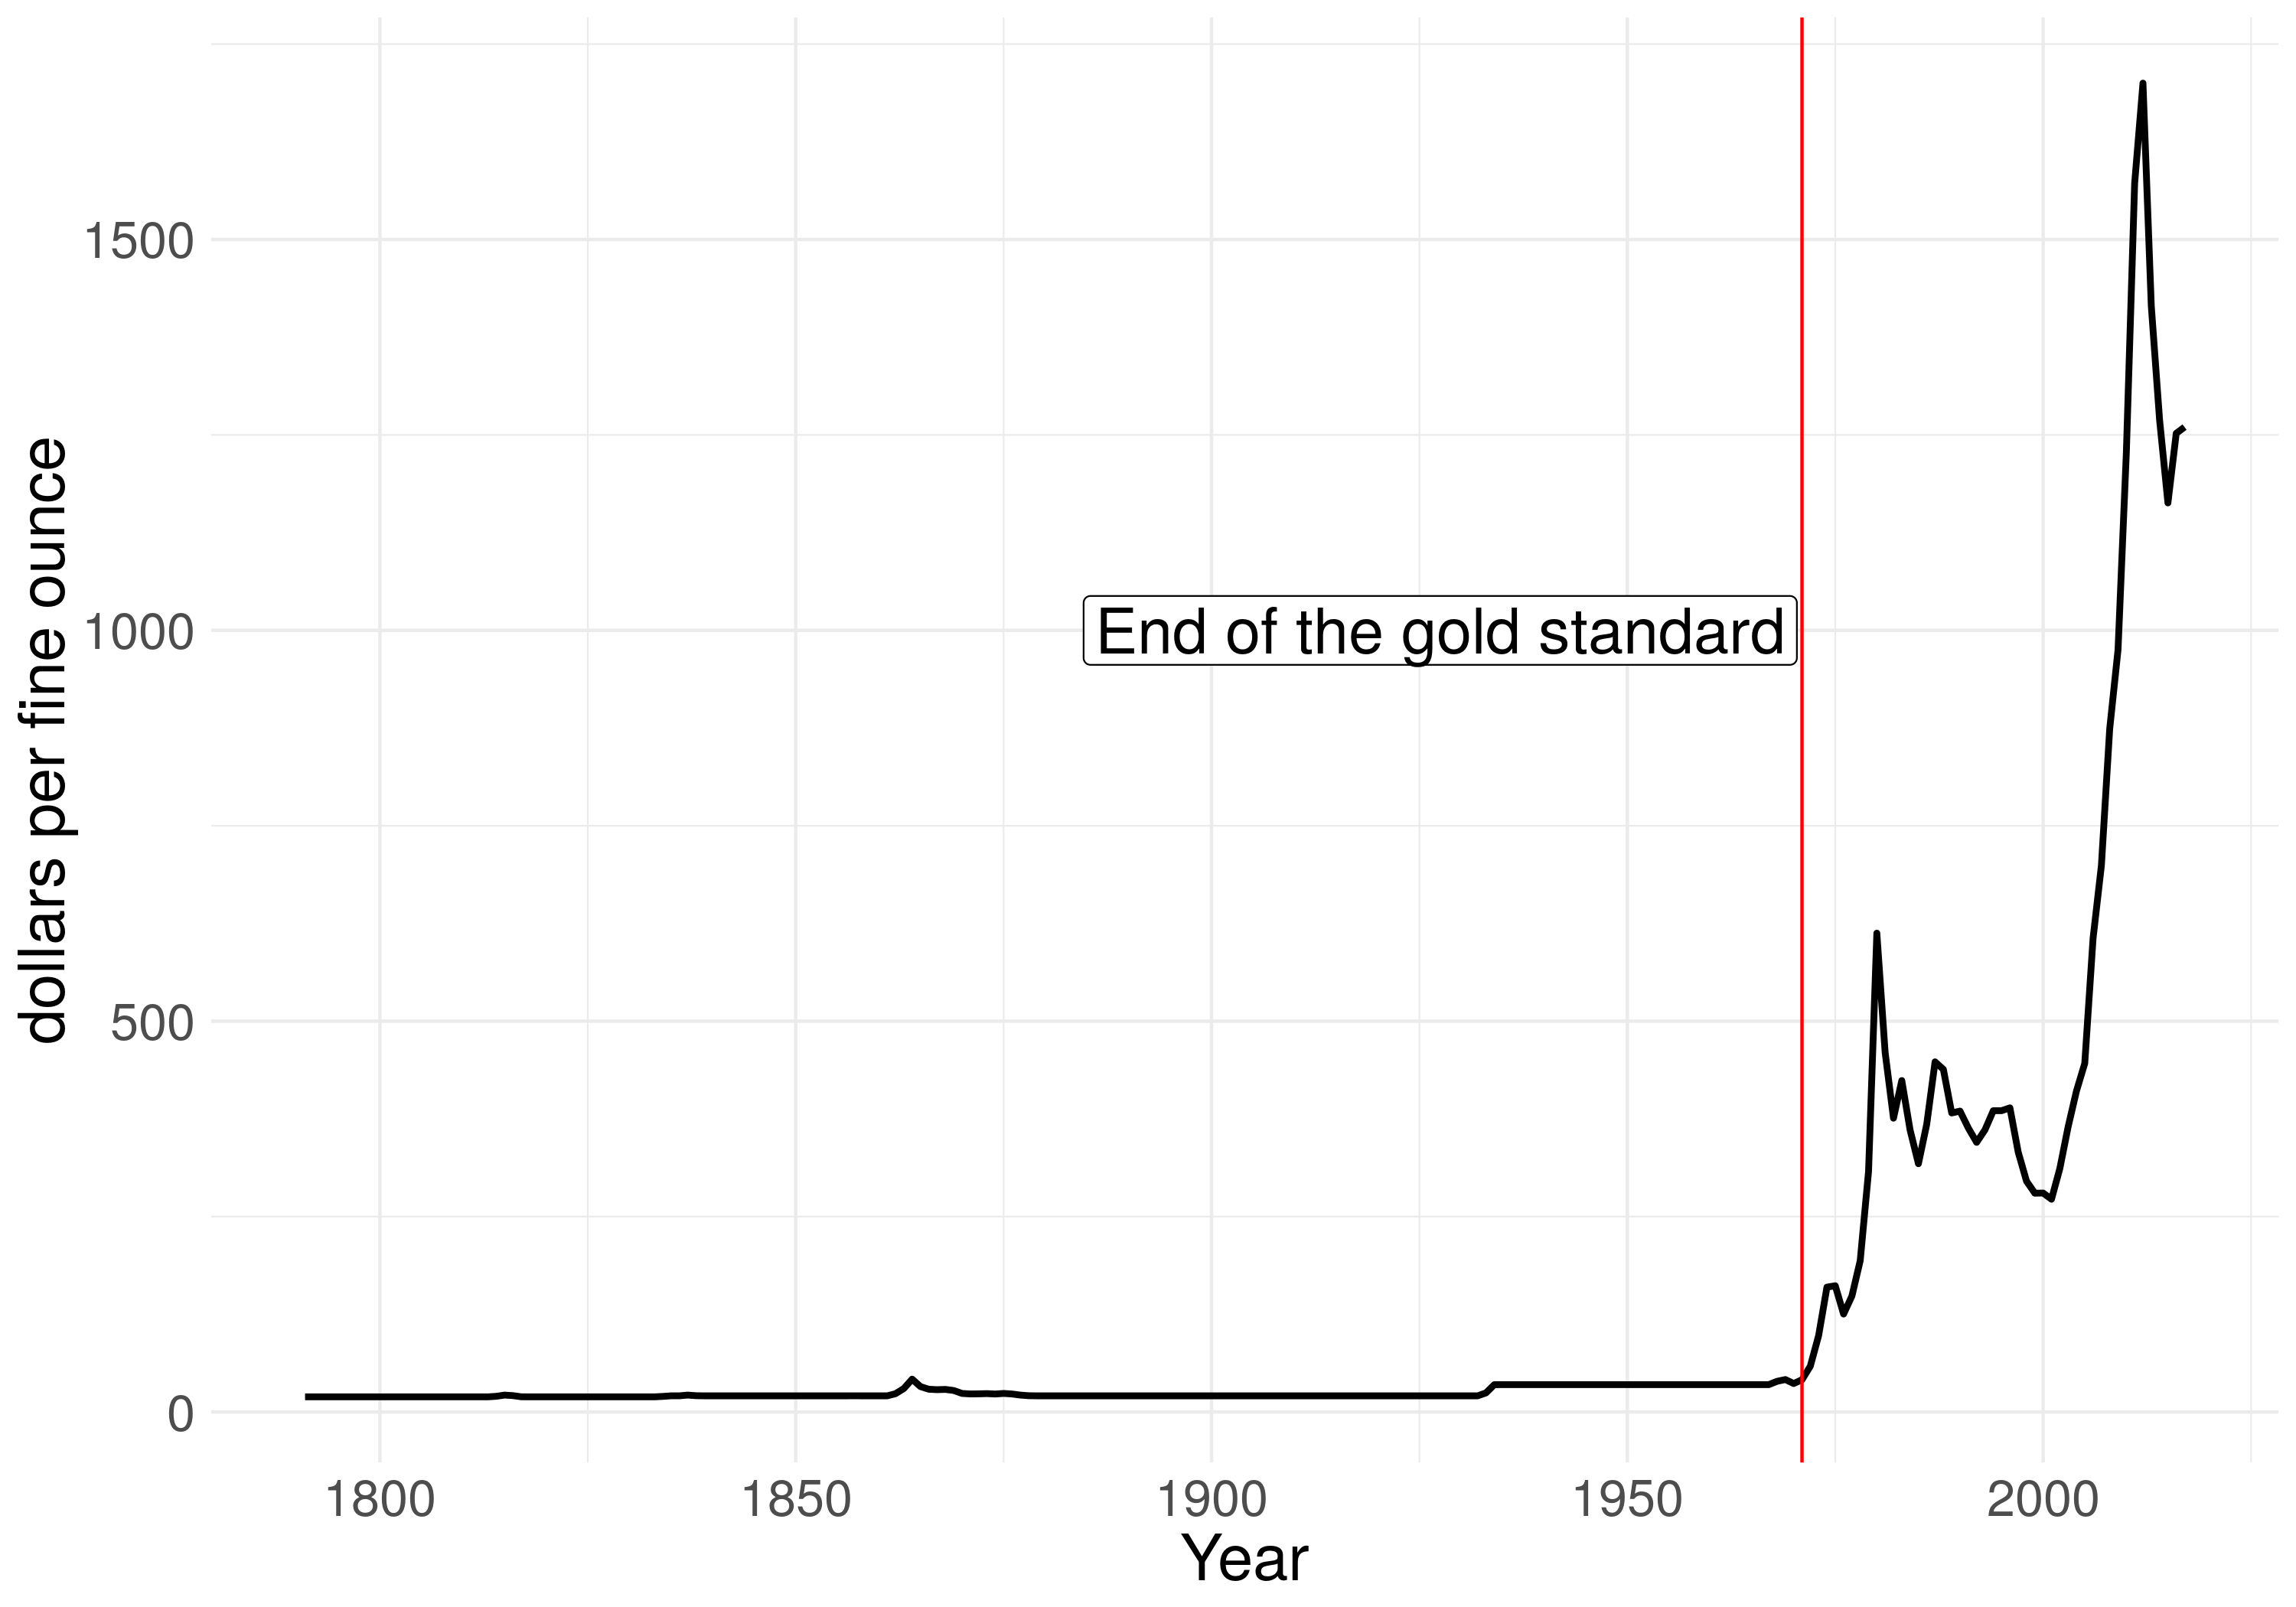
\includegraphics[width=0.75\linewidth]{oro_en.png}
%		\caption{Gold prices New York Market. Price per ounce. 1790-2017}\label{fig:oro}
%	\end{figure}


	\begin{figure}[H]
	\centering
	\subfigure[New York Market. Price per ounce. 1790-2017]{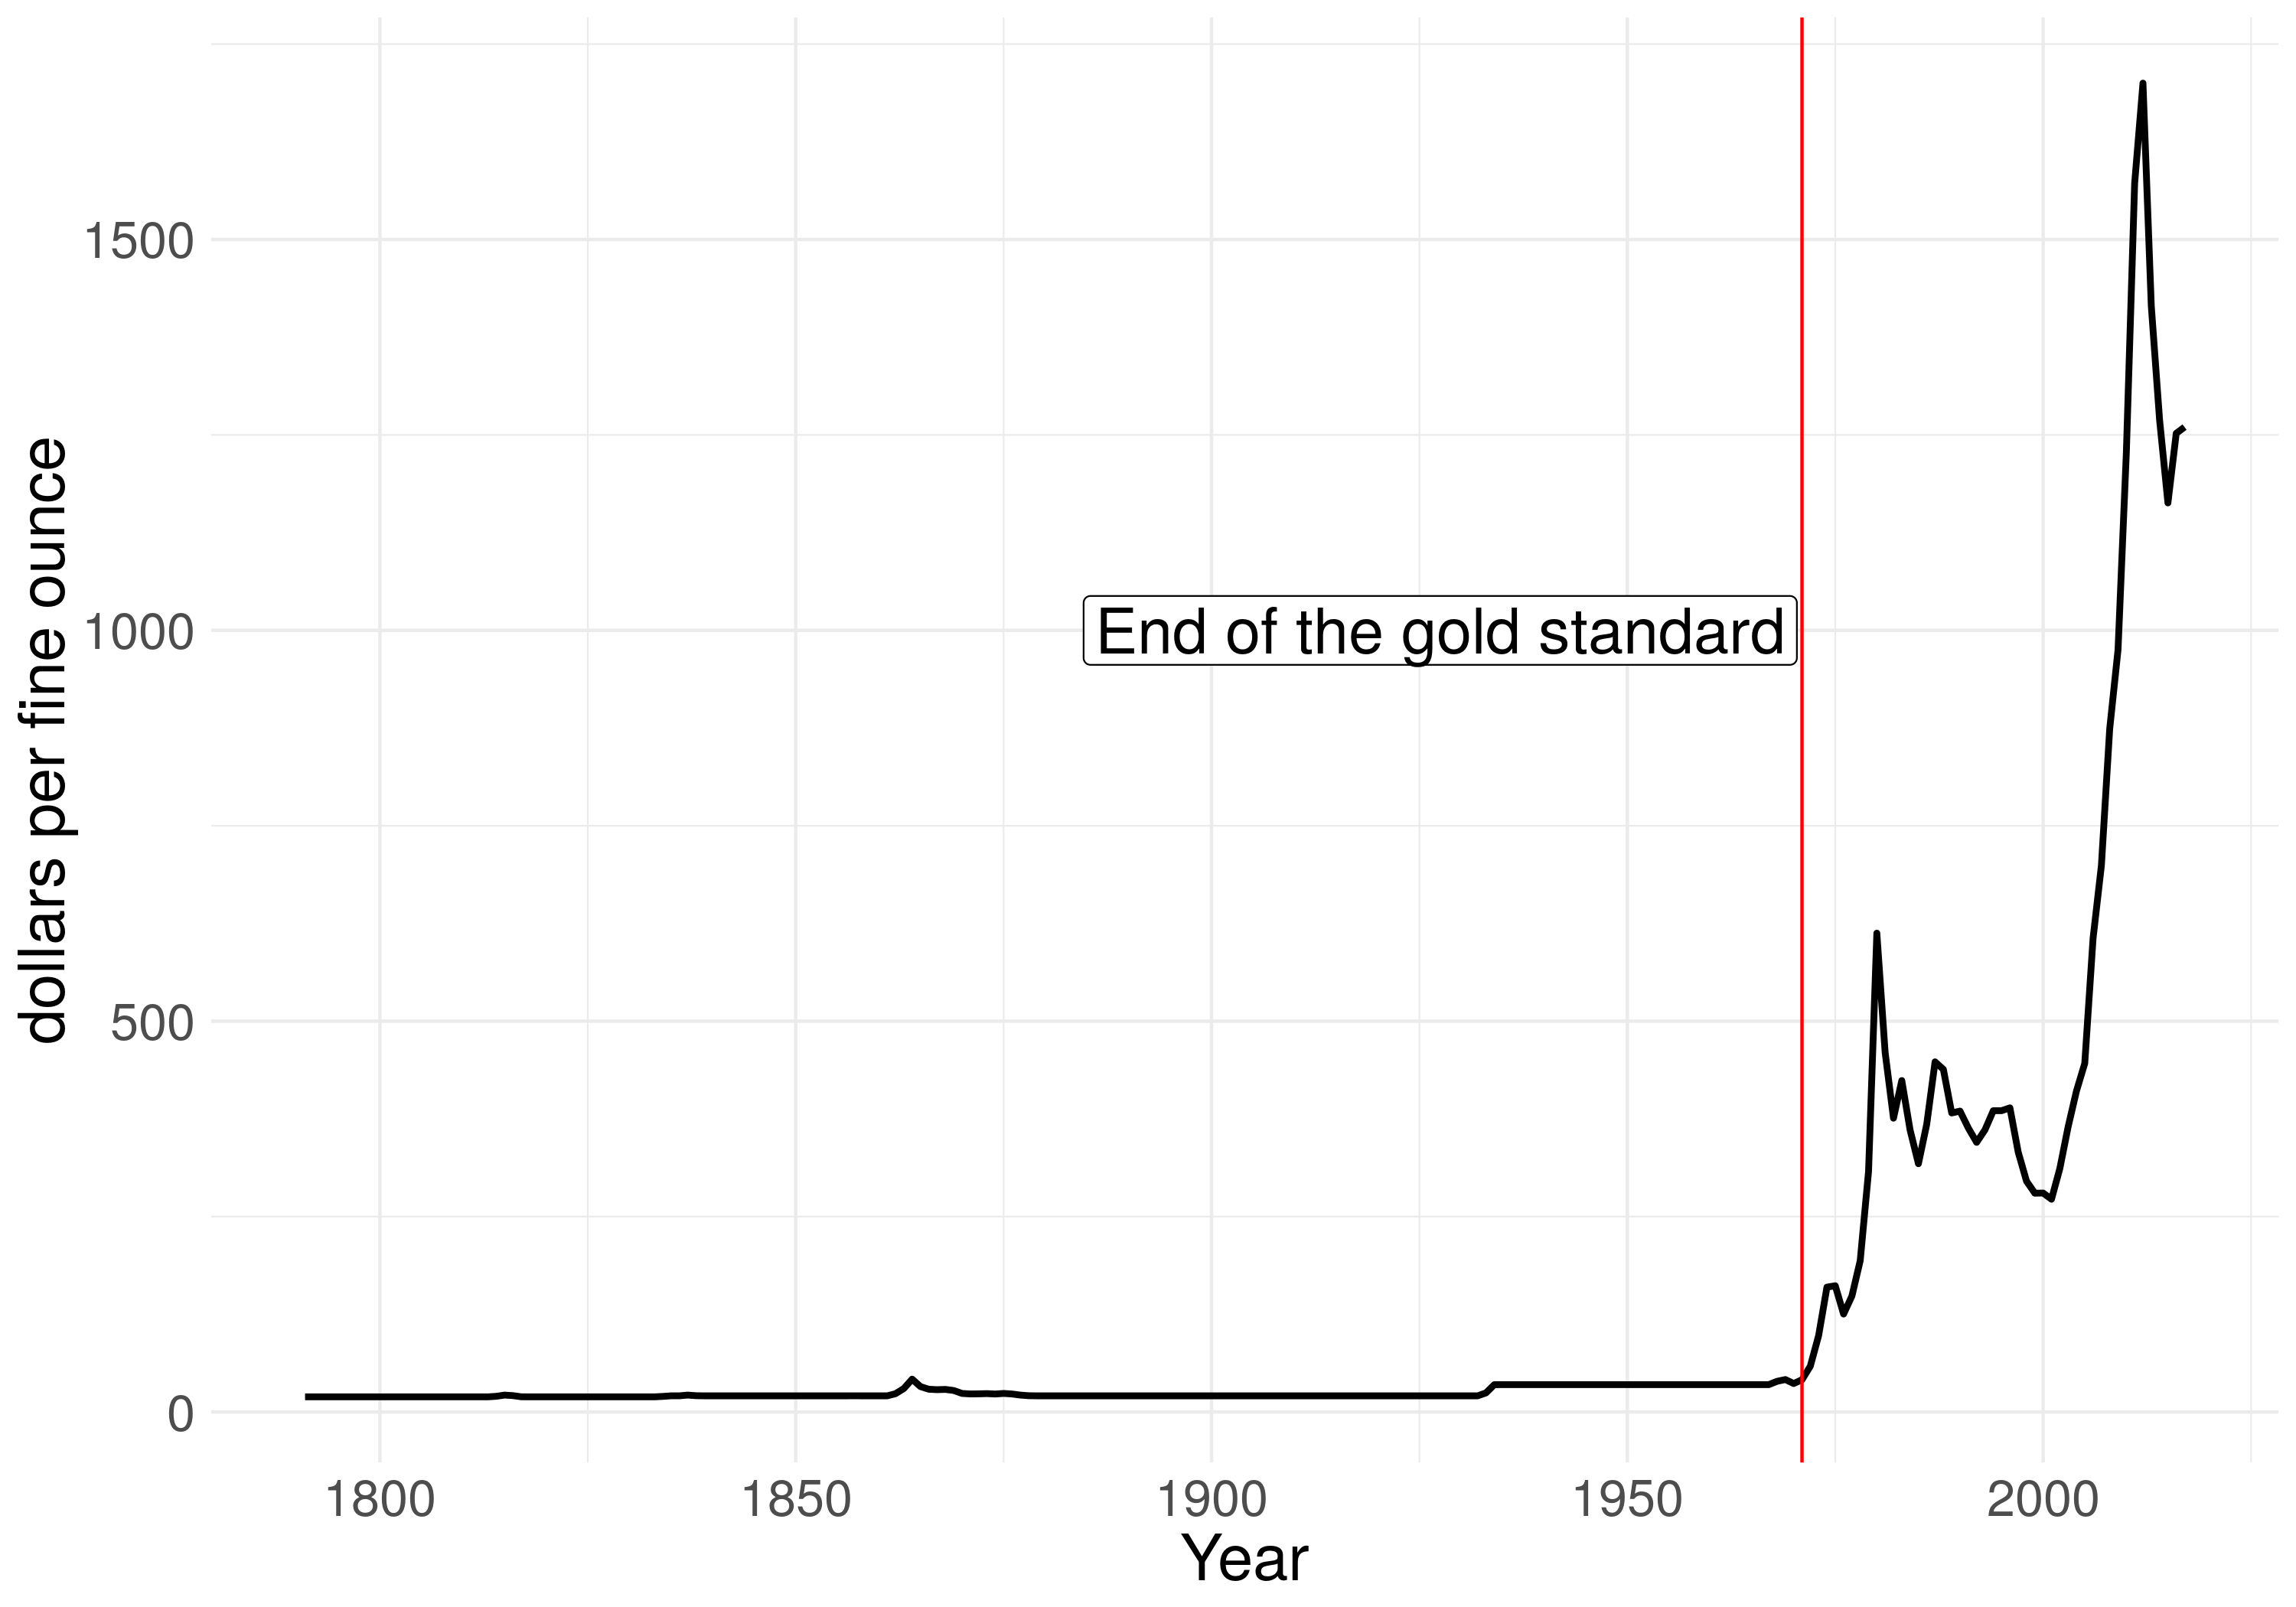
\includegraphics[width=0.75\linewidth]{oro_en.PNG}
		\label{fig:oro_us}}
	\subfigure[London Market. British pounds per ounce. 1700-1900]{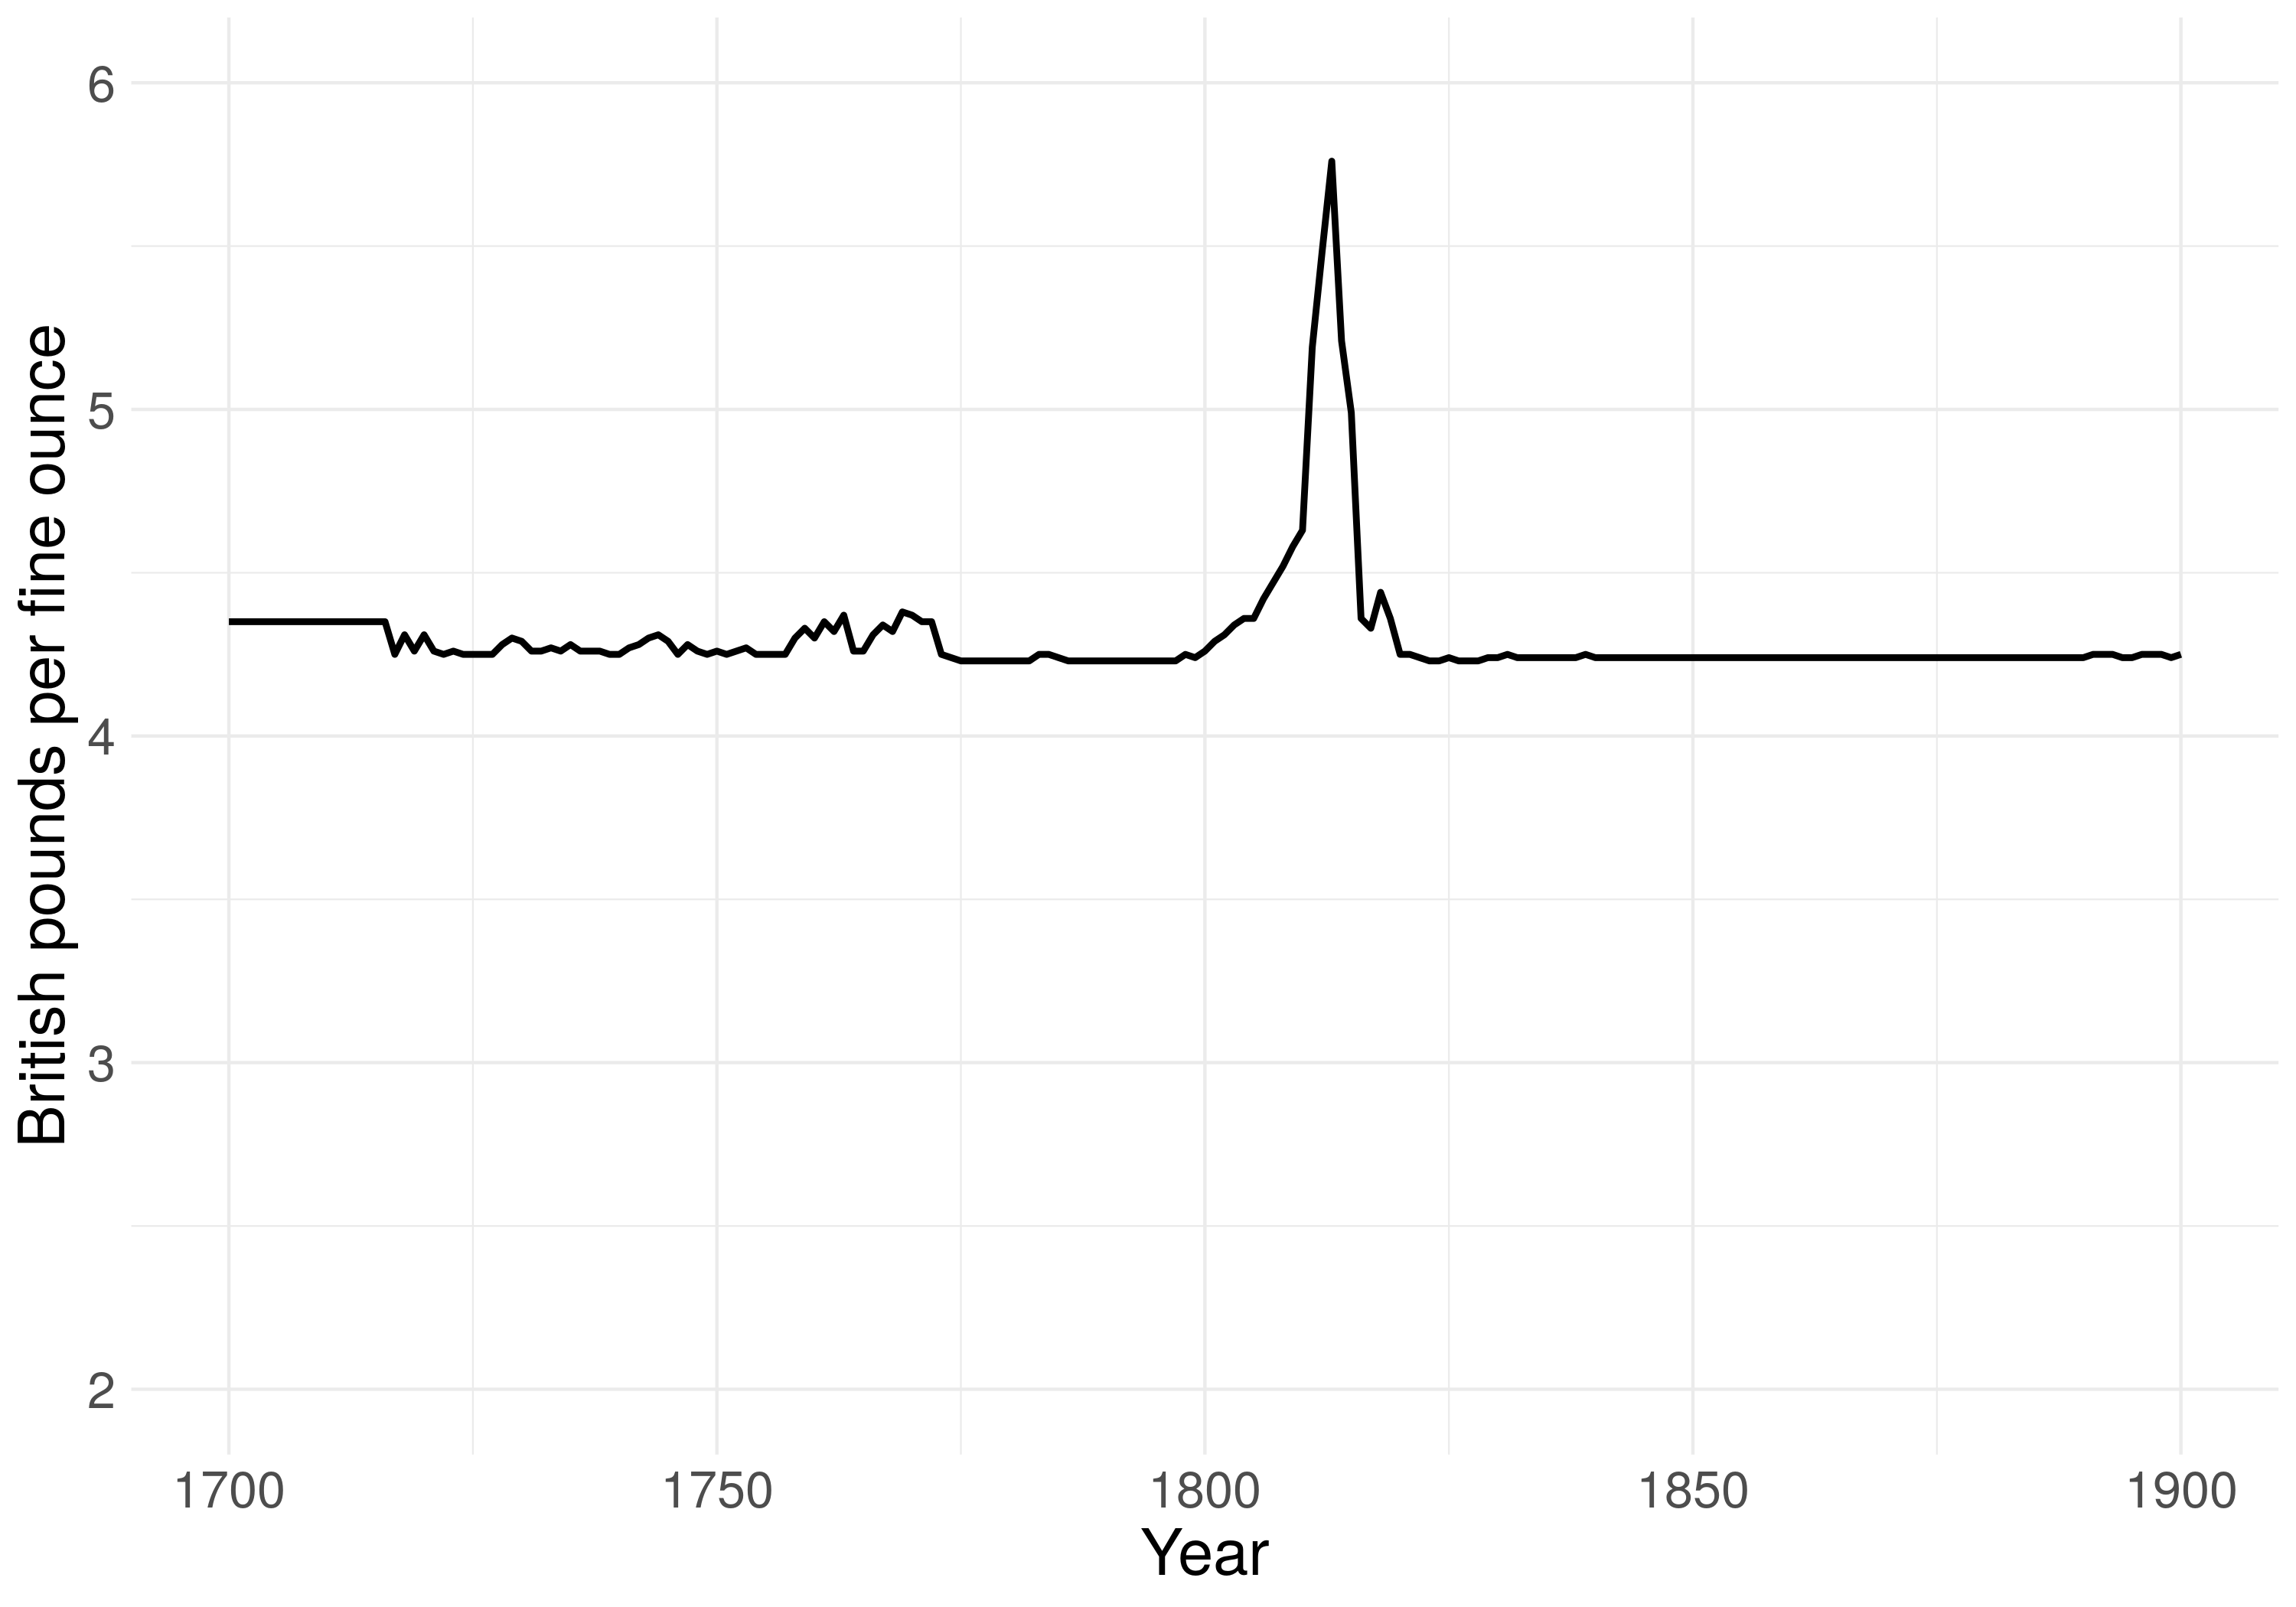
\includegraphics[width=0.75\linewidth]{oro_uk.PNG}
		\label{fig:oro_uk}}
	\caption{Gold prices.} \label{fig:oro}
\end{figure}
	
	Given that what we sought in this paper is a long-term analysis of the economic cycle, this nominal disturbance obscures the underlying phenomenon. That is why we choose to normalize the nominal GDP series and the nominal wage by the price of gold. In this sense, we can read the series as the product and wage expressed in its capacity to purchase gold.
	
	
	Since gold is a refuge of value in crisis periods, its price is counter-cyclical, a difference from what happens with the Consumer Price Index (CPI). Therefore normalizing by gold instead of CPI gives a better comprehension of the cycle in the series and facilitate the empirical analysis.
	
	According to the above, the figure \ref{fig:PBI} shows the series of the United States GDP between 1900 and 2017, expressed in gold. Meanwhile, the figure \ref{fig:salario} shows the series of the hourly wage of a worker of production in the United States between 1900 and 2017, also expressed in gold.
	
	In both cases, the periods of economic distress known by the literature are highlighted in red, and in punctuated lines those specific crises that occurred in a particular year. The table \ref{tabla_crisis} marks the detail of these.
	
	
	\begin{figure}[H]
		\centering
		\subfigure[US GDP. Millions of ounces of gold, 1900-2017]{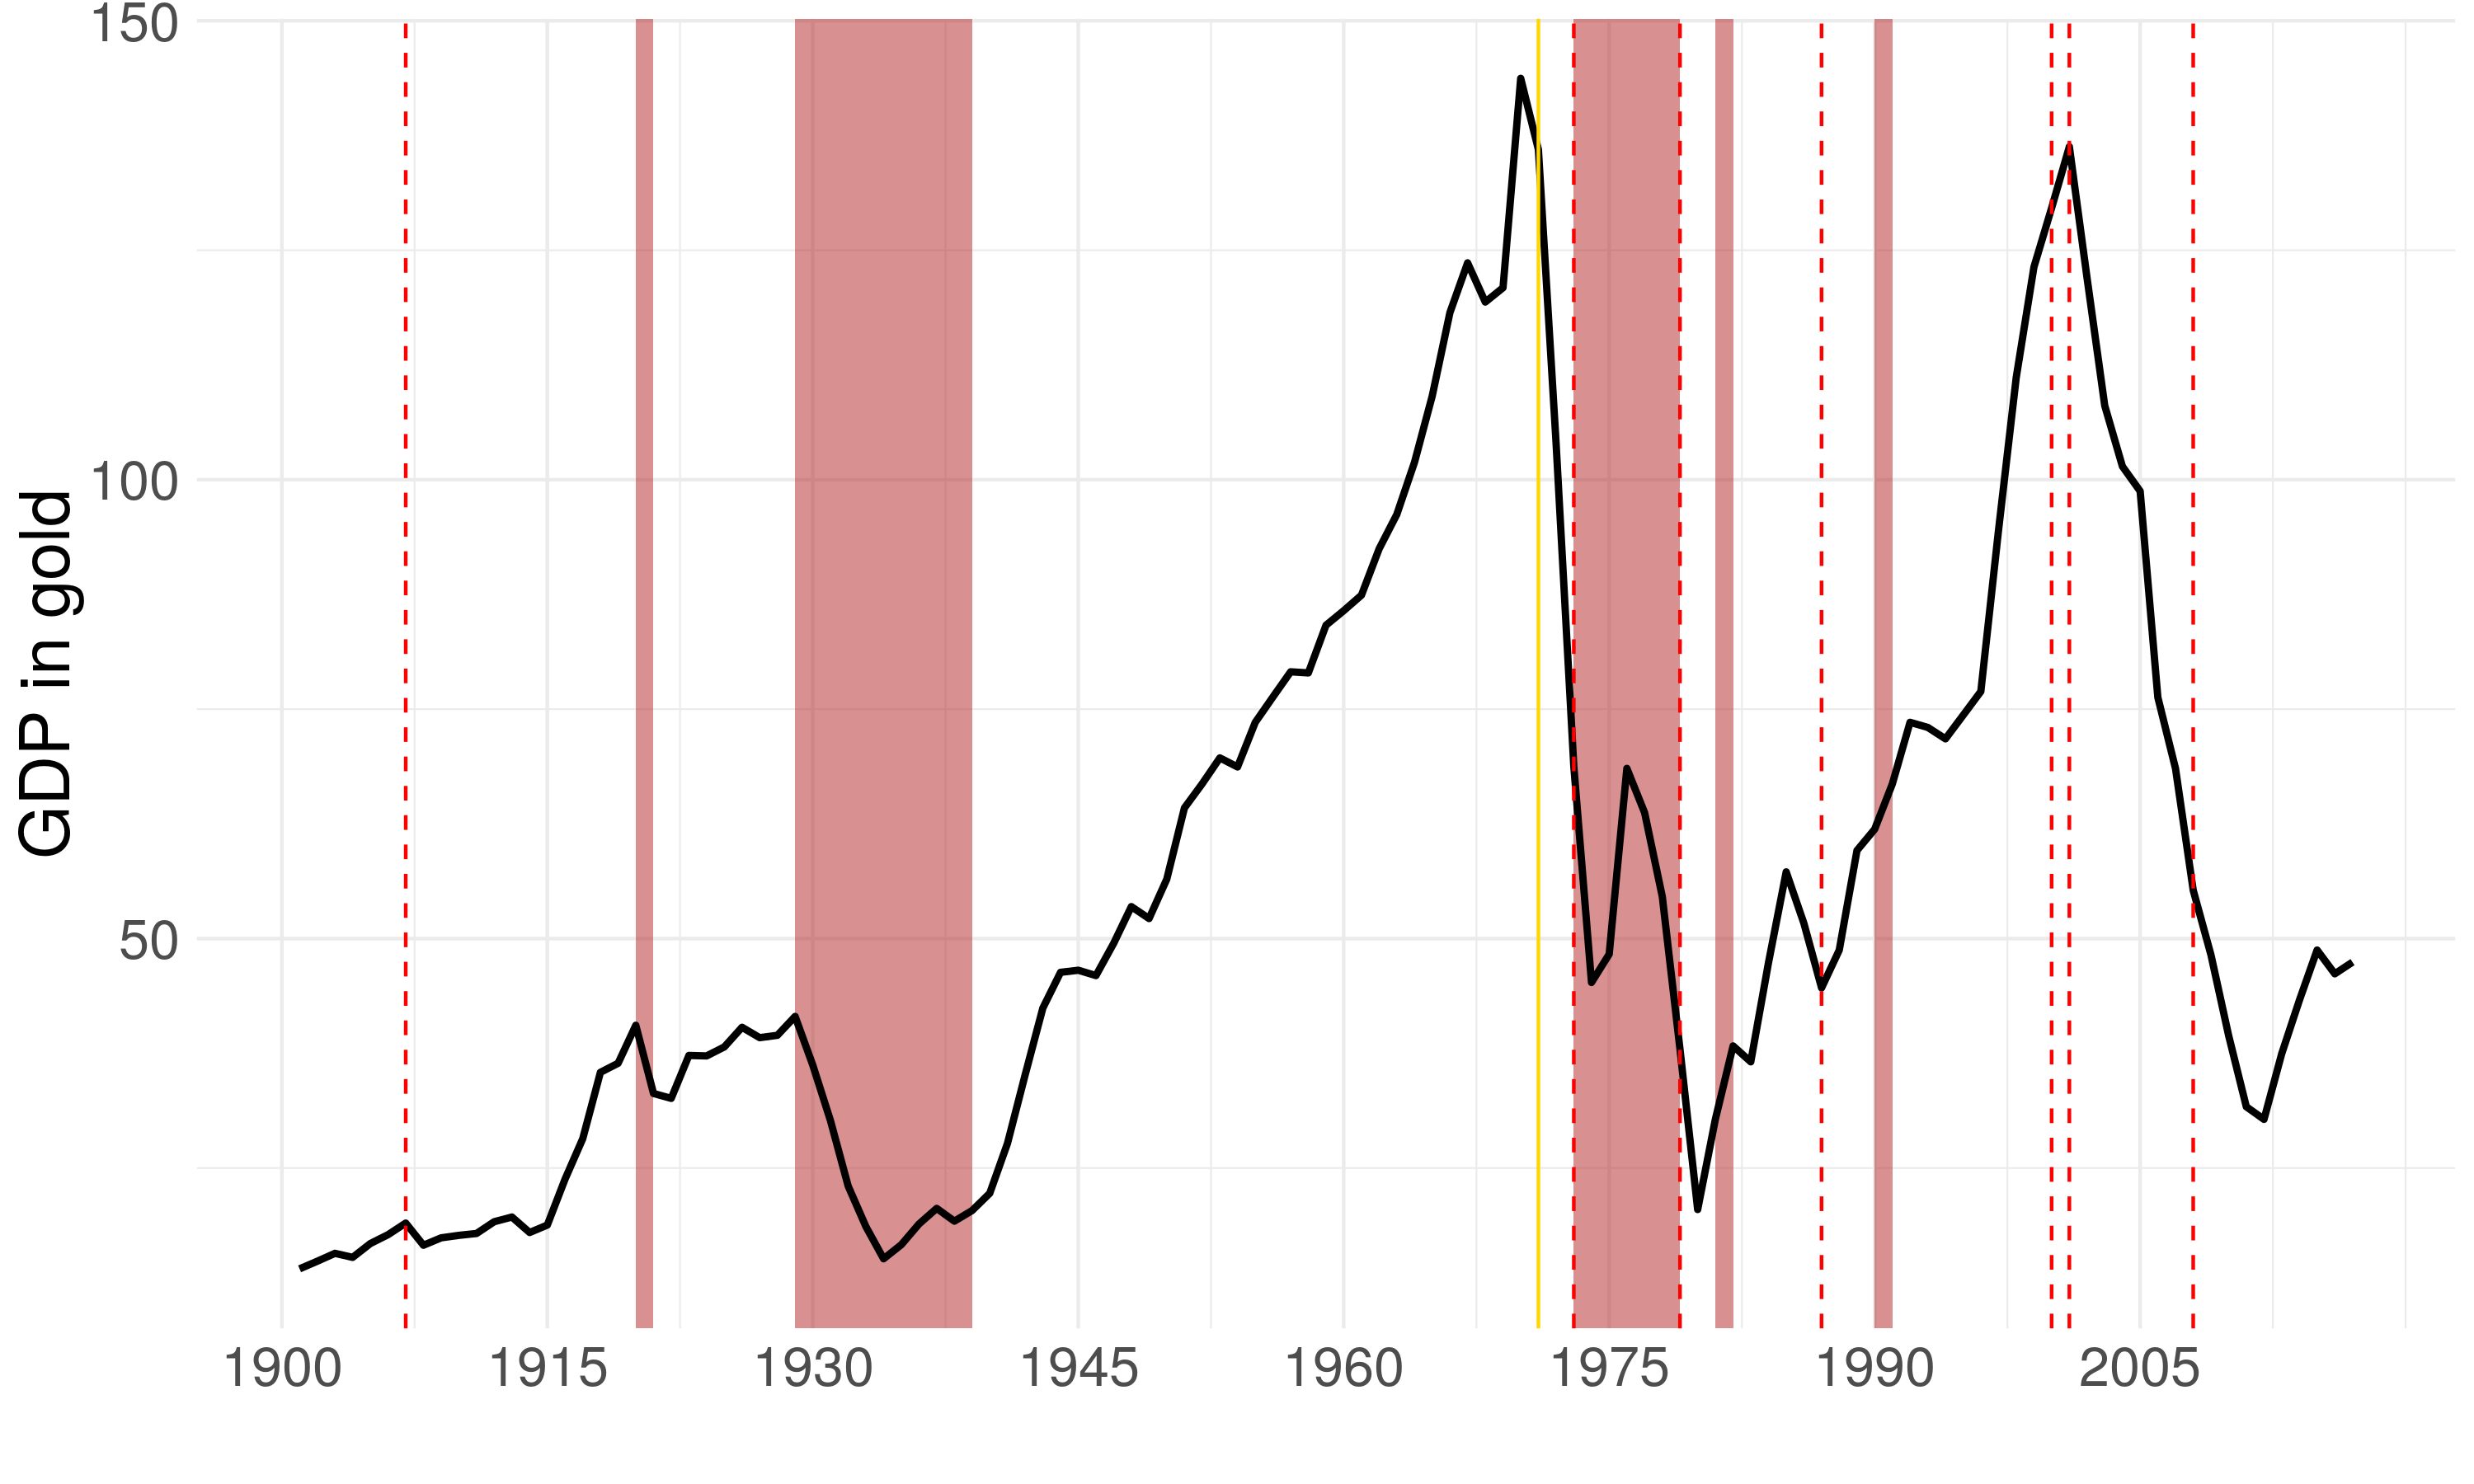
\includegraphics[width=0.75\linewidth]{gdp_in_gold_eda_en.PNG}
			\label{fig:PBI}}
		\subfigure[US Hourly Wage. Ounces of gold, 1900-2017]{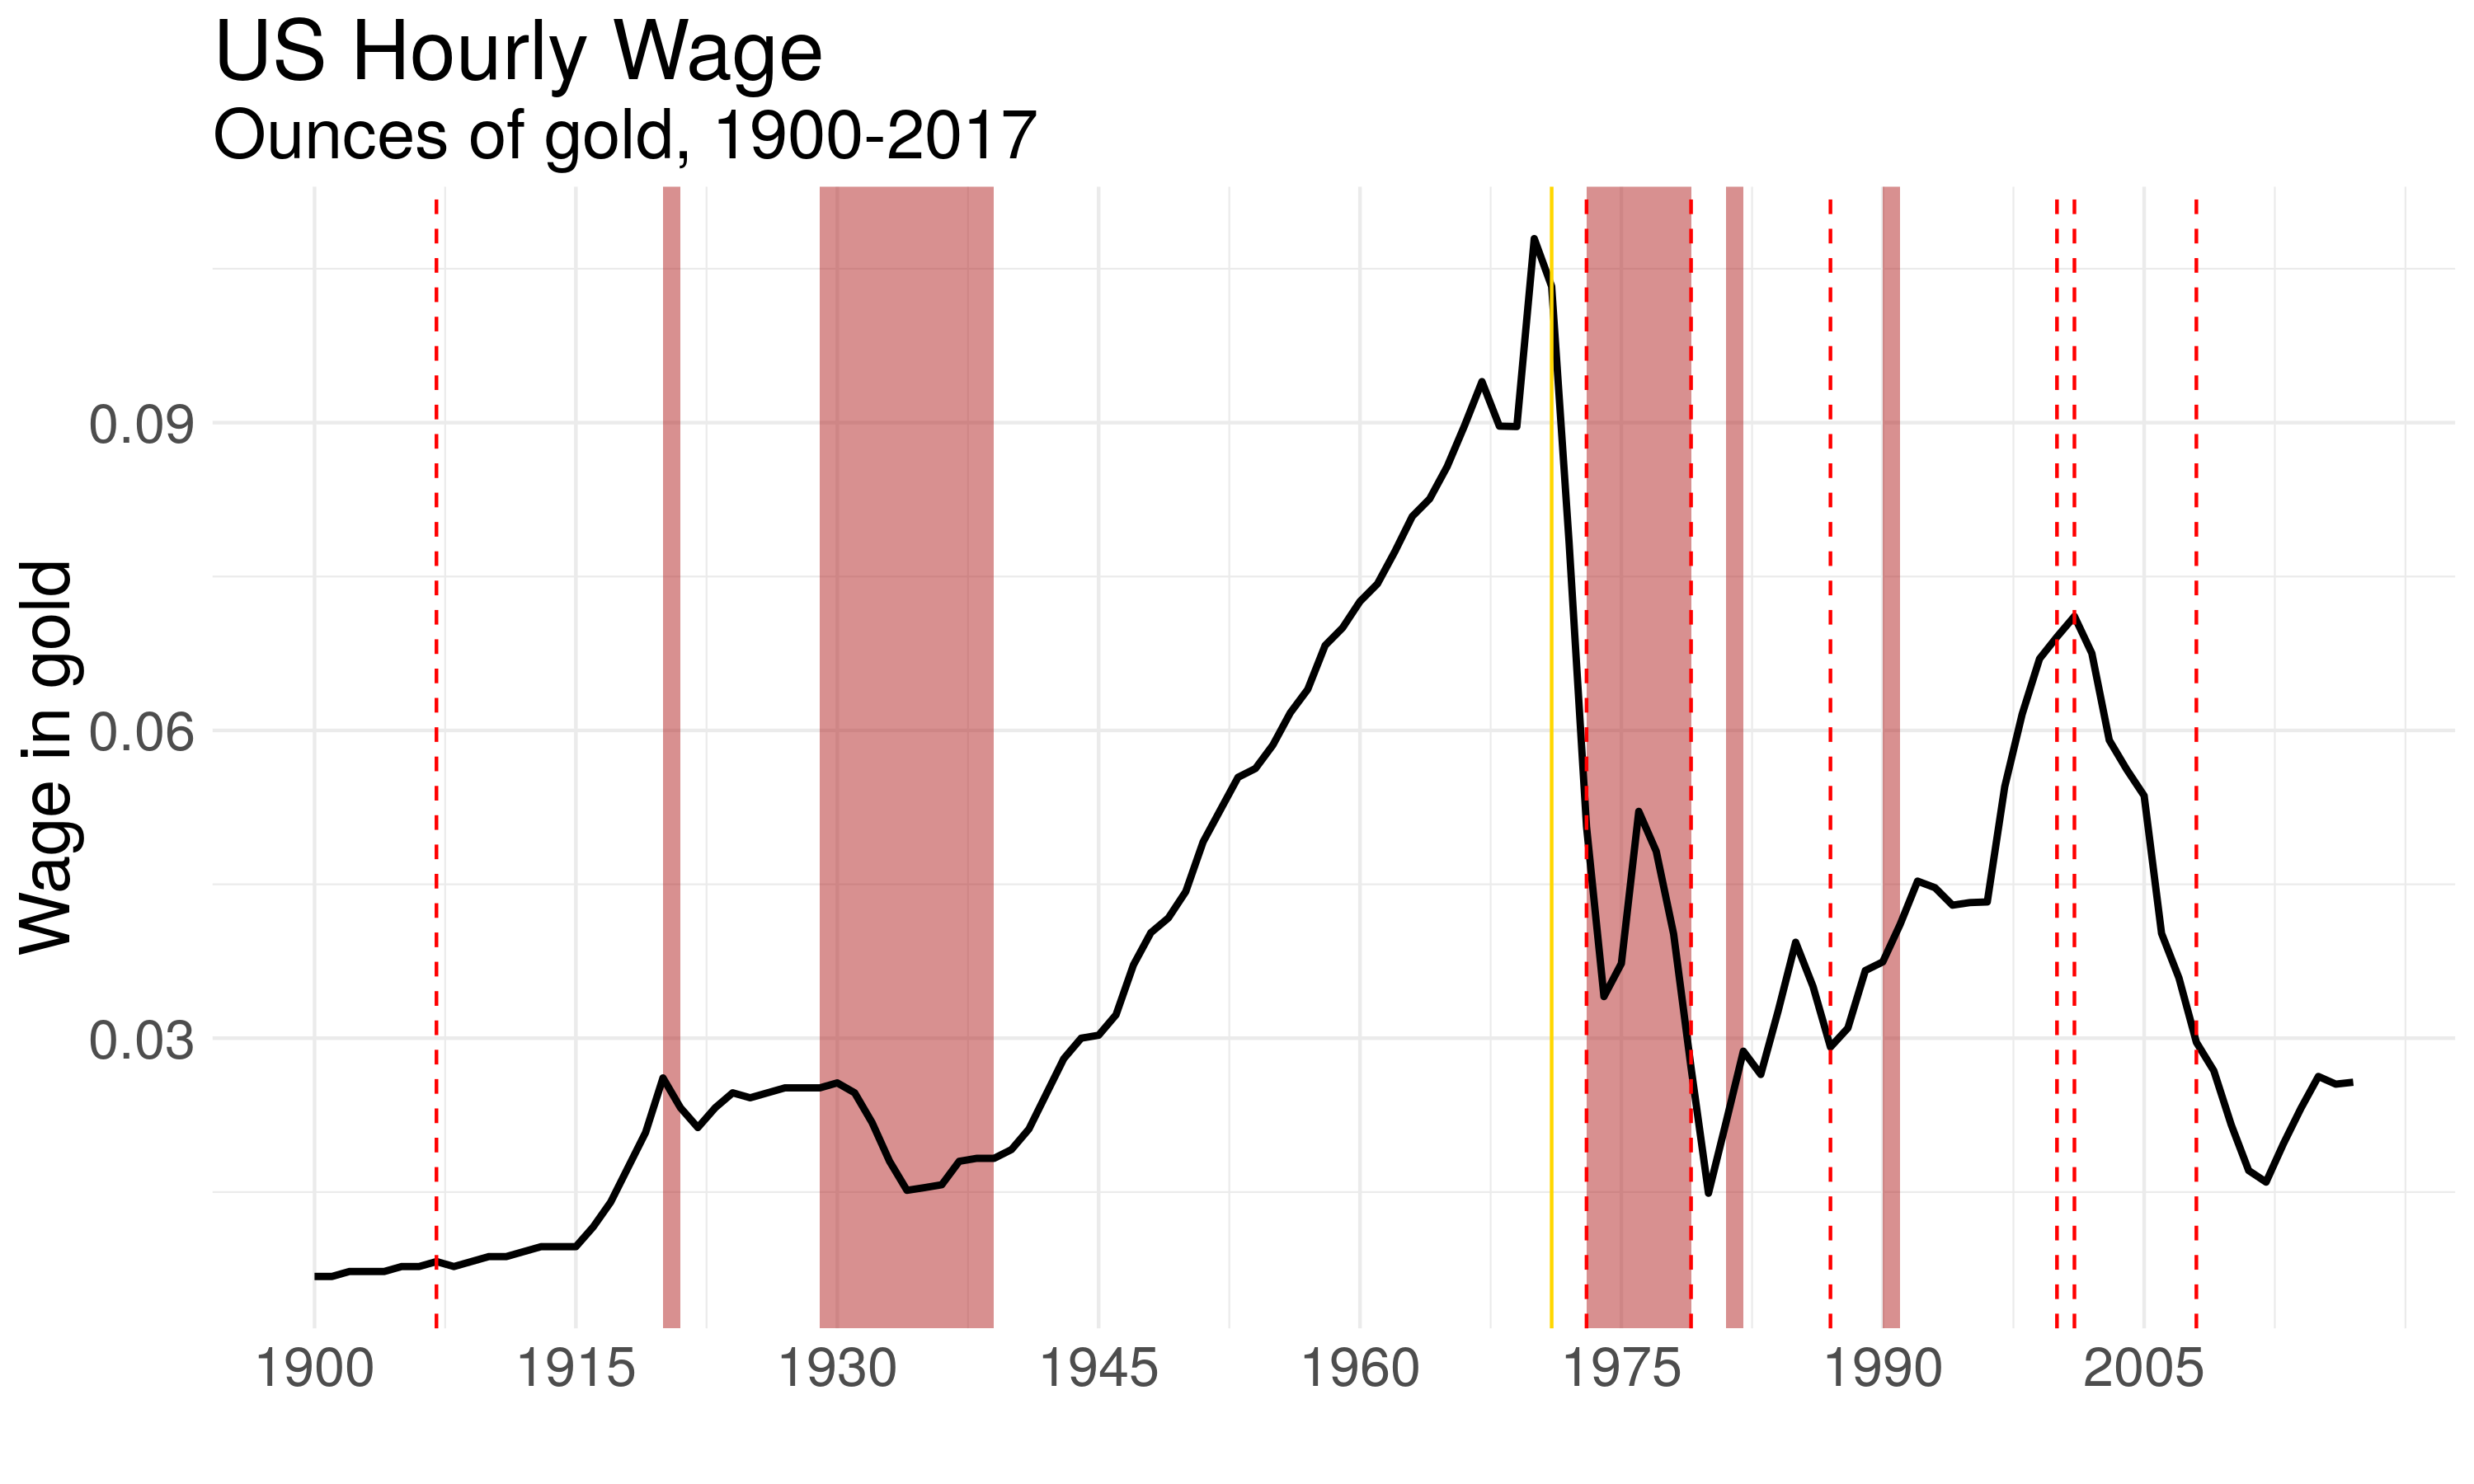
\includegraphics[width=0.75\linewidth]{wg_in_gold_eda_en.PNG}
			\label{fig:salario}}
		\caption{GDP and Wage. US. Crisis highlighted} \label{fig:series_crisis}
	\end{figure}
	
	
	\begin{table}[ht]
		\centering
		\begin{tabular}{ll}
			\hline
			Period & Crisis \\ 
			\hline
			1907 & Panic of 1907 \\ 
			1920 – 1921 & Depression of 1920 – 21 \\ 
			1929 – 1939 & Great Depression \\ 
			1970s & 1970s Energy Crisis \\ 
			1973 & OPEC Oil Price Shock \\ 
			1979 & Iranian Revolution\\ 
			1980s & Early 1980s Recession\\ 
			1987 & Black Monday \\ 
			1990s & Early 1990s Recession\\ 
			2000 & Dot-com Bubble \\ 
			2001 & 911 \\ 
			2008 & Subprime Global Financial Crisis \\ 
			\hline
		\end{tabular}
		\caption{Main US and Global Crisis during 20th century.}
		\label{tabla_crisis}
	\end{table}
	
	We can observe the similarity of both series. Both show three peaks, during the 20', in 1970 and 2000, followed by deep falls. The normalization by the gold-price allows seeing a great cycle with three oscillations, at least apparently, during the twentieth century. The crises reviewed by the economic history literature seem to have their correlate in the movements observed in both series. Besides, it is also interesting to note that the third upward movement, whose peak is in the year 2000, leads to a value similar to that of the previous oscillatory movement for the case of GDP, but not for wages. This latter expresses that the distribution of the GDP between wage and profit has changed in the last period.
	
	As a complement of the United States's series is interesting to observe the movement of the product at the United Kingdom for the other centenaries. During the eighteenth and nineteenth centuries this country was parapet as the core of global accumulation, and therefore it may be possible to find evidence of the economic cycle in this country in particular. The figure \ref{fig:uk_gdp} shows the GDP of the United Kingdom, between 1700 and 1900. It is normalized by the price of gold in the London market from 1718, while the first years correspond to the official British price. At the same time, the years of fall of the GDP from 1800 are stood out, given that for the eighteenth century there are no visually outstanding points.
	
	\begin{figure}[H]
		\centering
		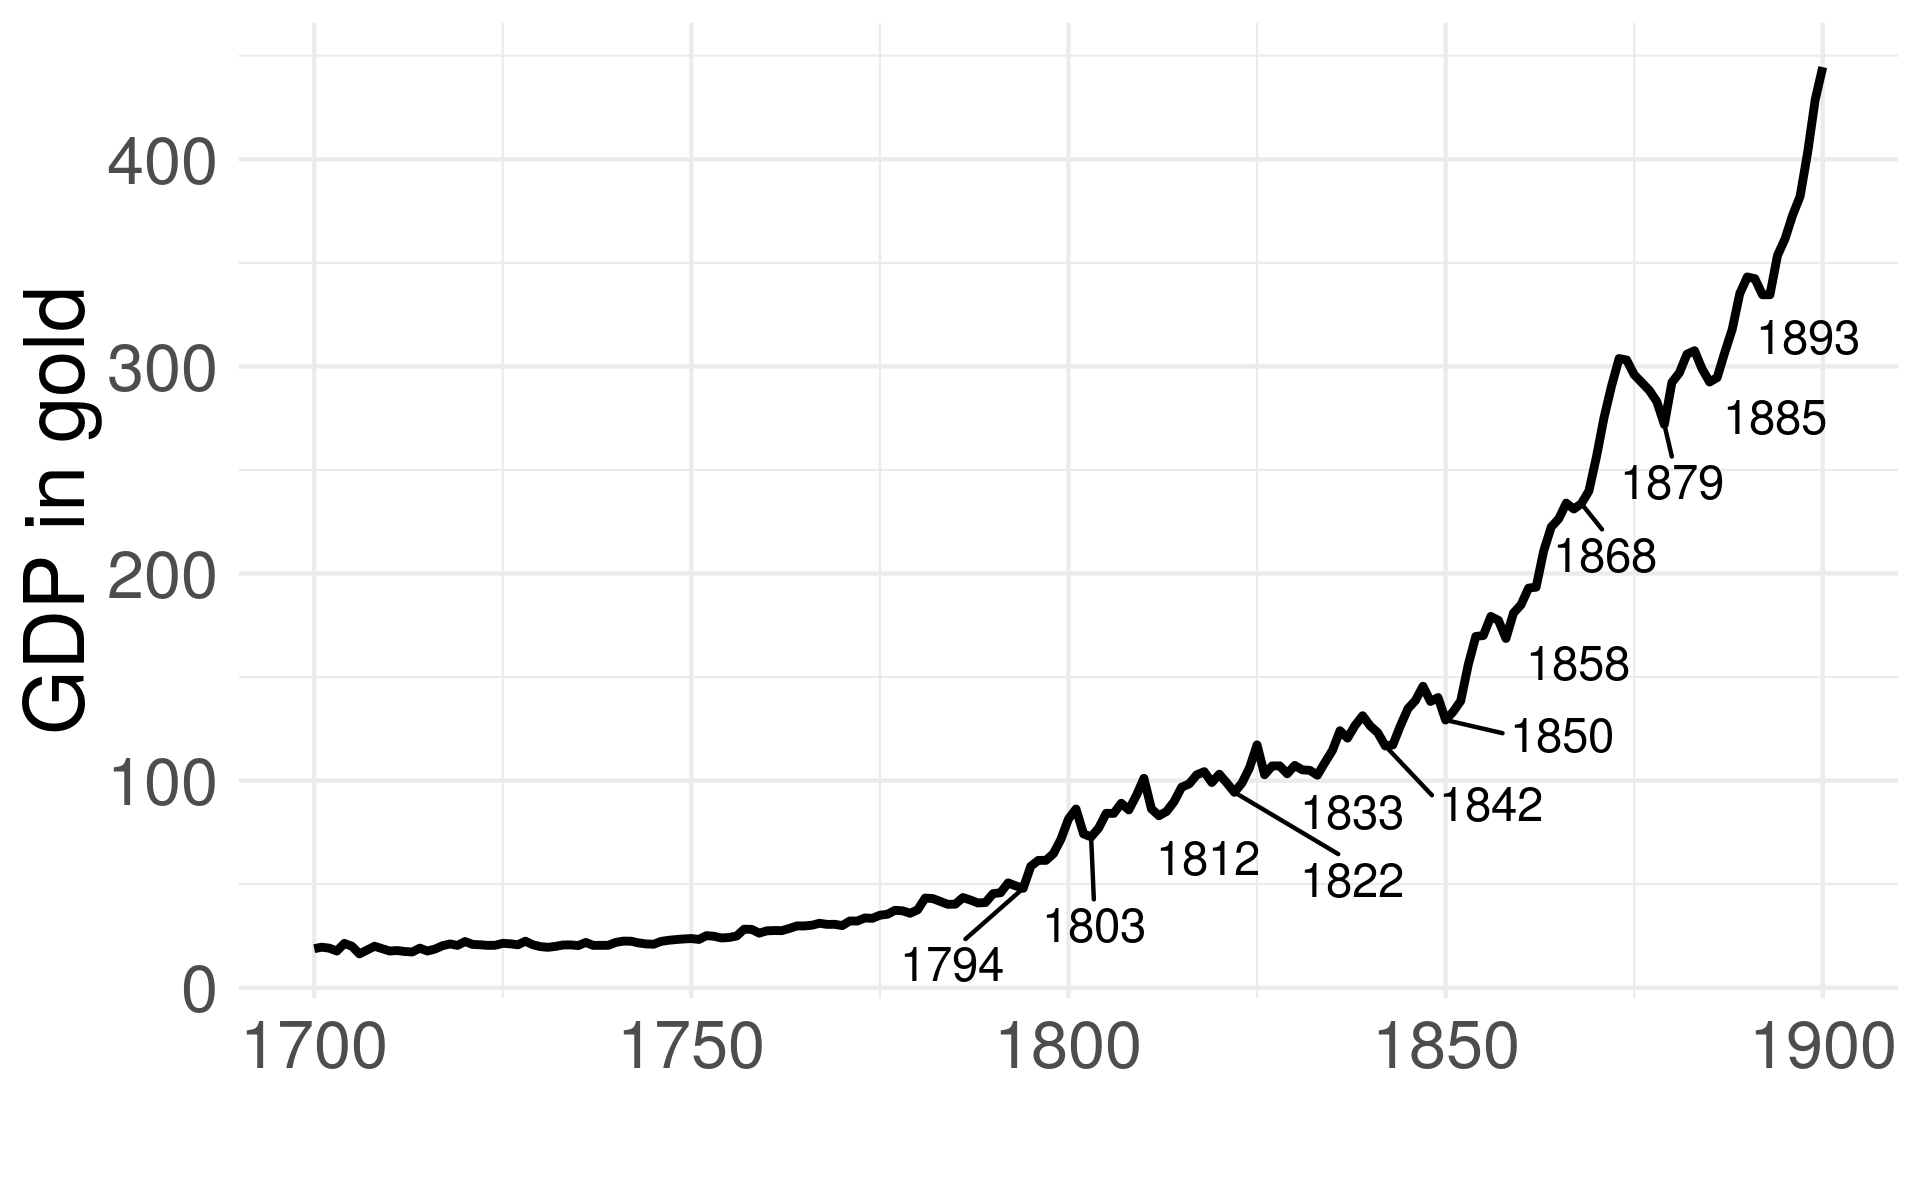
\includegraphics[width=0.75\linewidth]{uk_gdp_en.png}
		\caption{UK GDP. Millions of ounces of gold. 1700-1900} 
		\label{fig:uk_gdp}
	\end{figure}
	
	
	We can see a softer upward movement than that seen in the 20th century. It is worth mentioning that the movement of the product in the United Kingdom during the twentieth century retains an essential similarity with that seen in the case of the United States. In the figure \ref{fig:uk_gdp}, however, a cyclic movement is observed of around ten years extension. During the nineteenth century, every seven to eleven years there is a fall in the product regarding its ability to buy gold. Just as the twentieth century accounts for three large oscillations, the nineteenth century marks the shorter oscillations, around ten years. For its part, The eighteenth century seems to be more stable.
	
	For completeness, we also show the available information for US and UK on the remaining periods. In figure \ref{fig:us_complement} we present the GDP and wages for US in gold, for the available period of 1791-1900. Here we can see that although both series share a similar trend, the detected crisis points in the GDP don't seem to be reflected, for the most of the cases, in the wages data. Also, we can see in \ref{fig:PBI_us_comp} that at the beginning of the period the crisis seemed to appear every twenty years, and from 1864, the inflection point appear every 5-10 years. 
	
	\begin{figure}[H]
		\centering
		\subfigure[US GDP. Millions of ounces of gold]{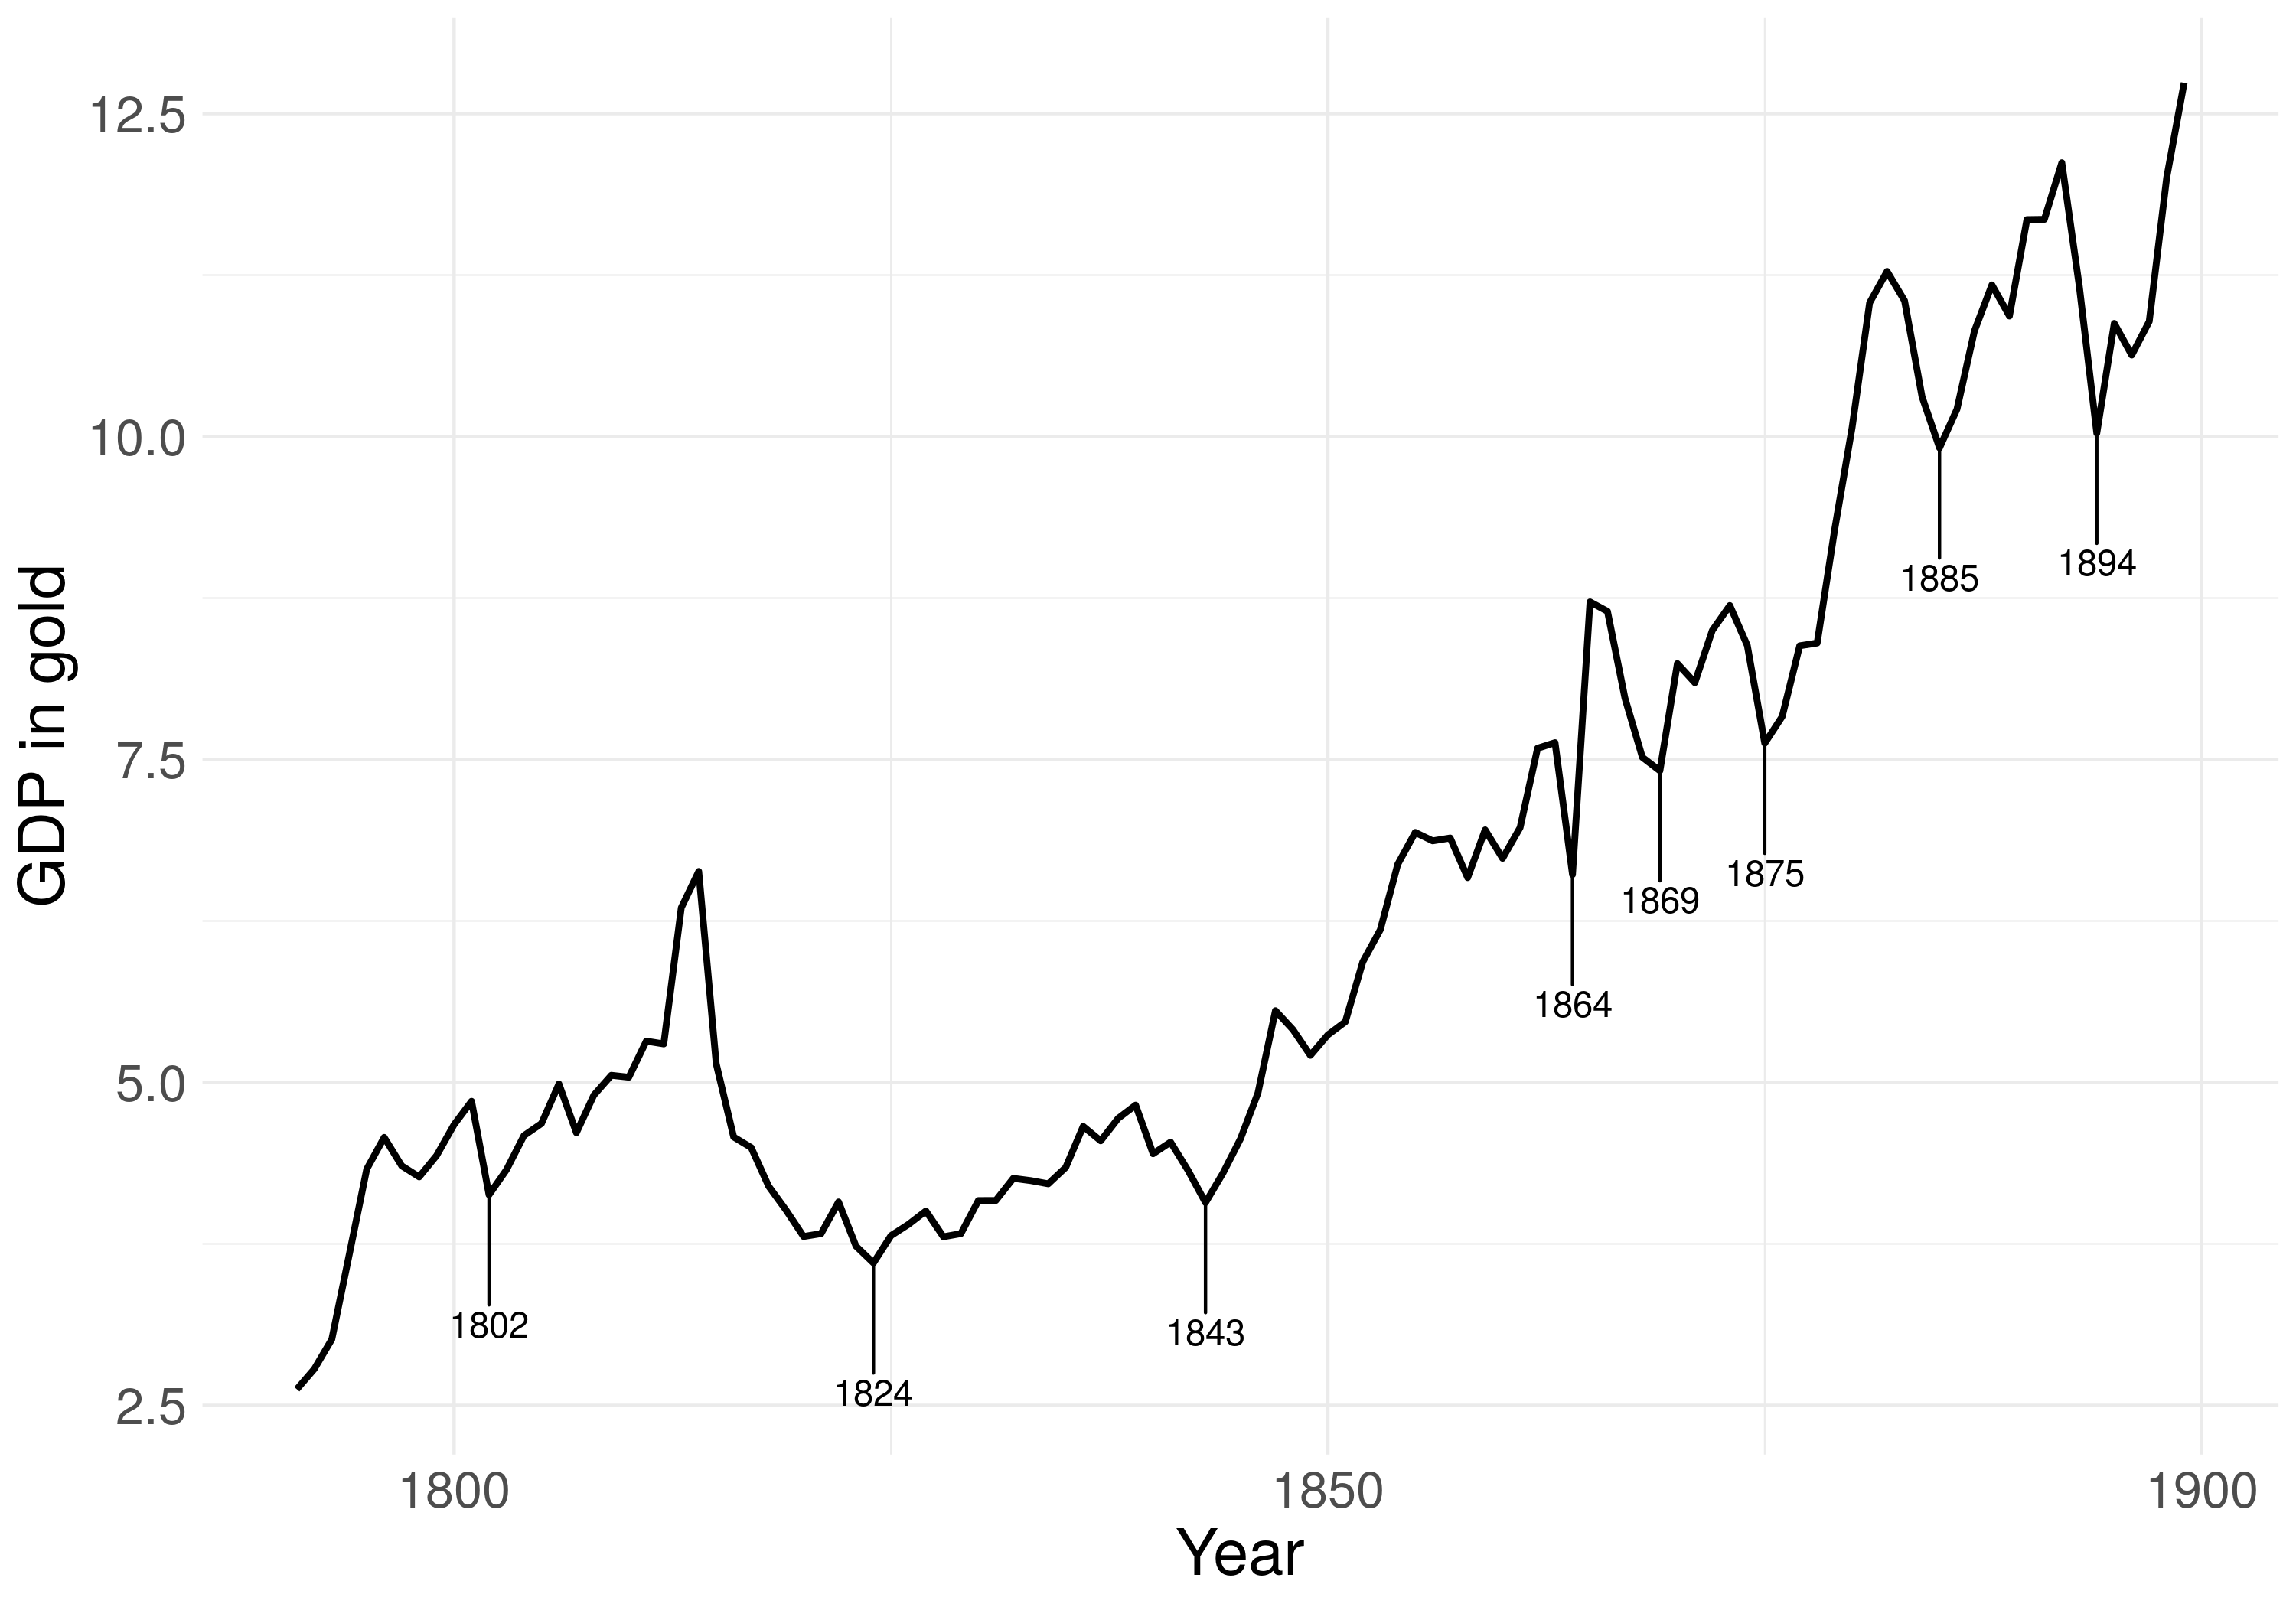
\includegraphics[width=0.75\linewidth]{gdp_us_complement.PNG}
			\label{fig:PBI_us_comp}}
		\subfigure[US Hourly Wage. Ounces of gold]{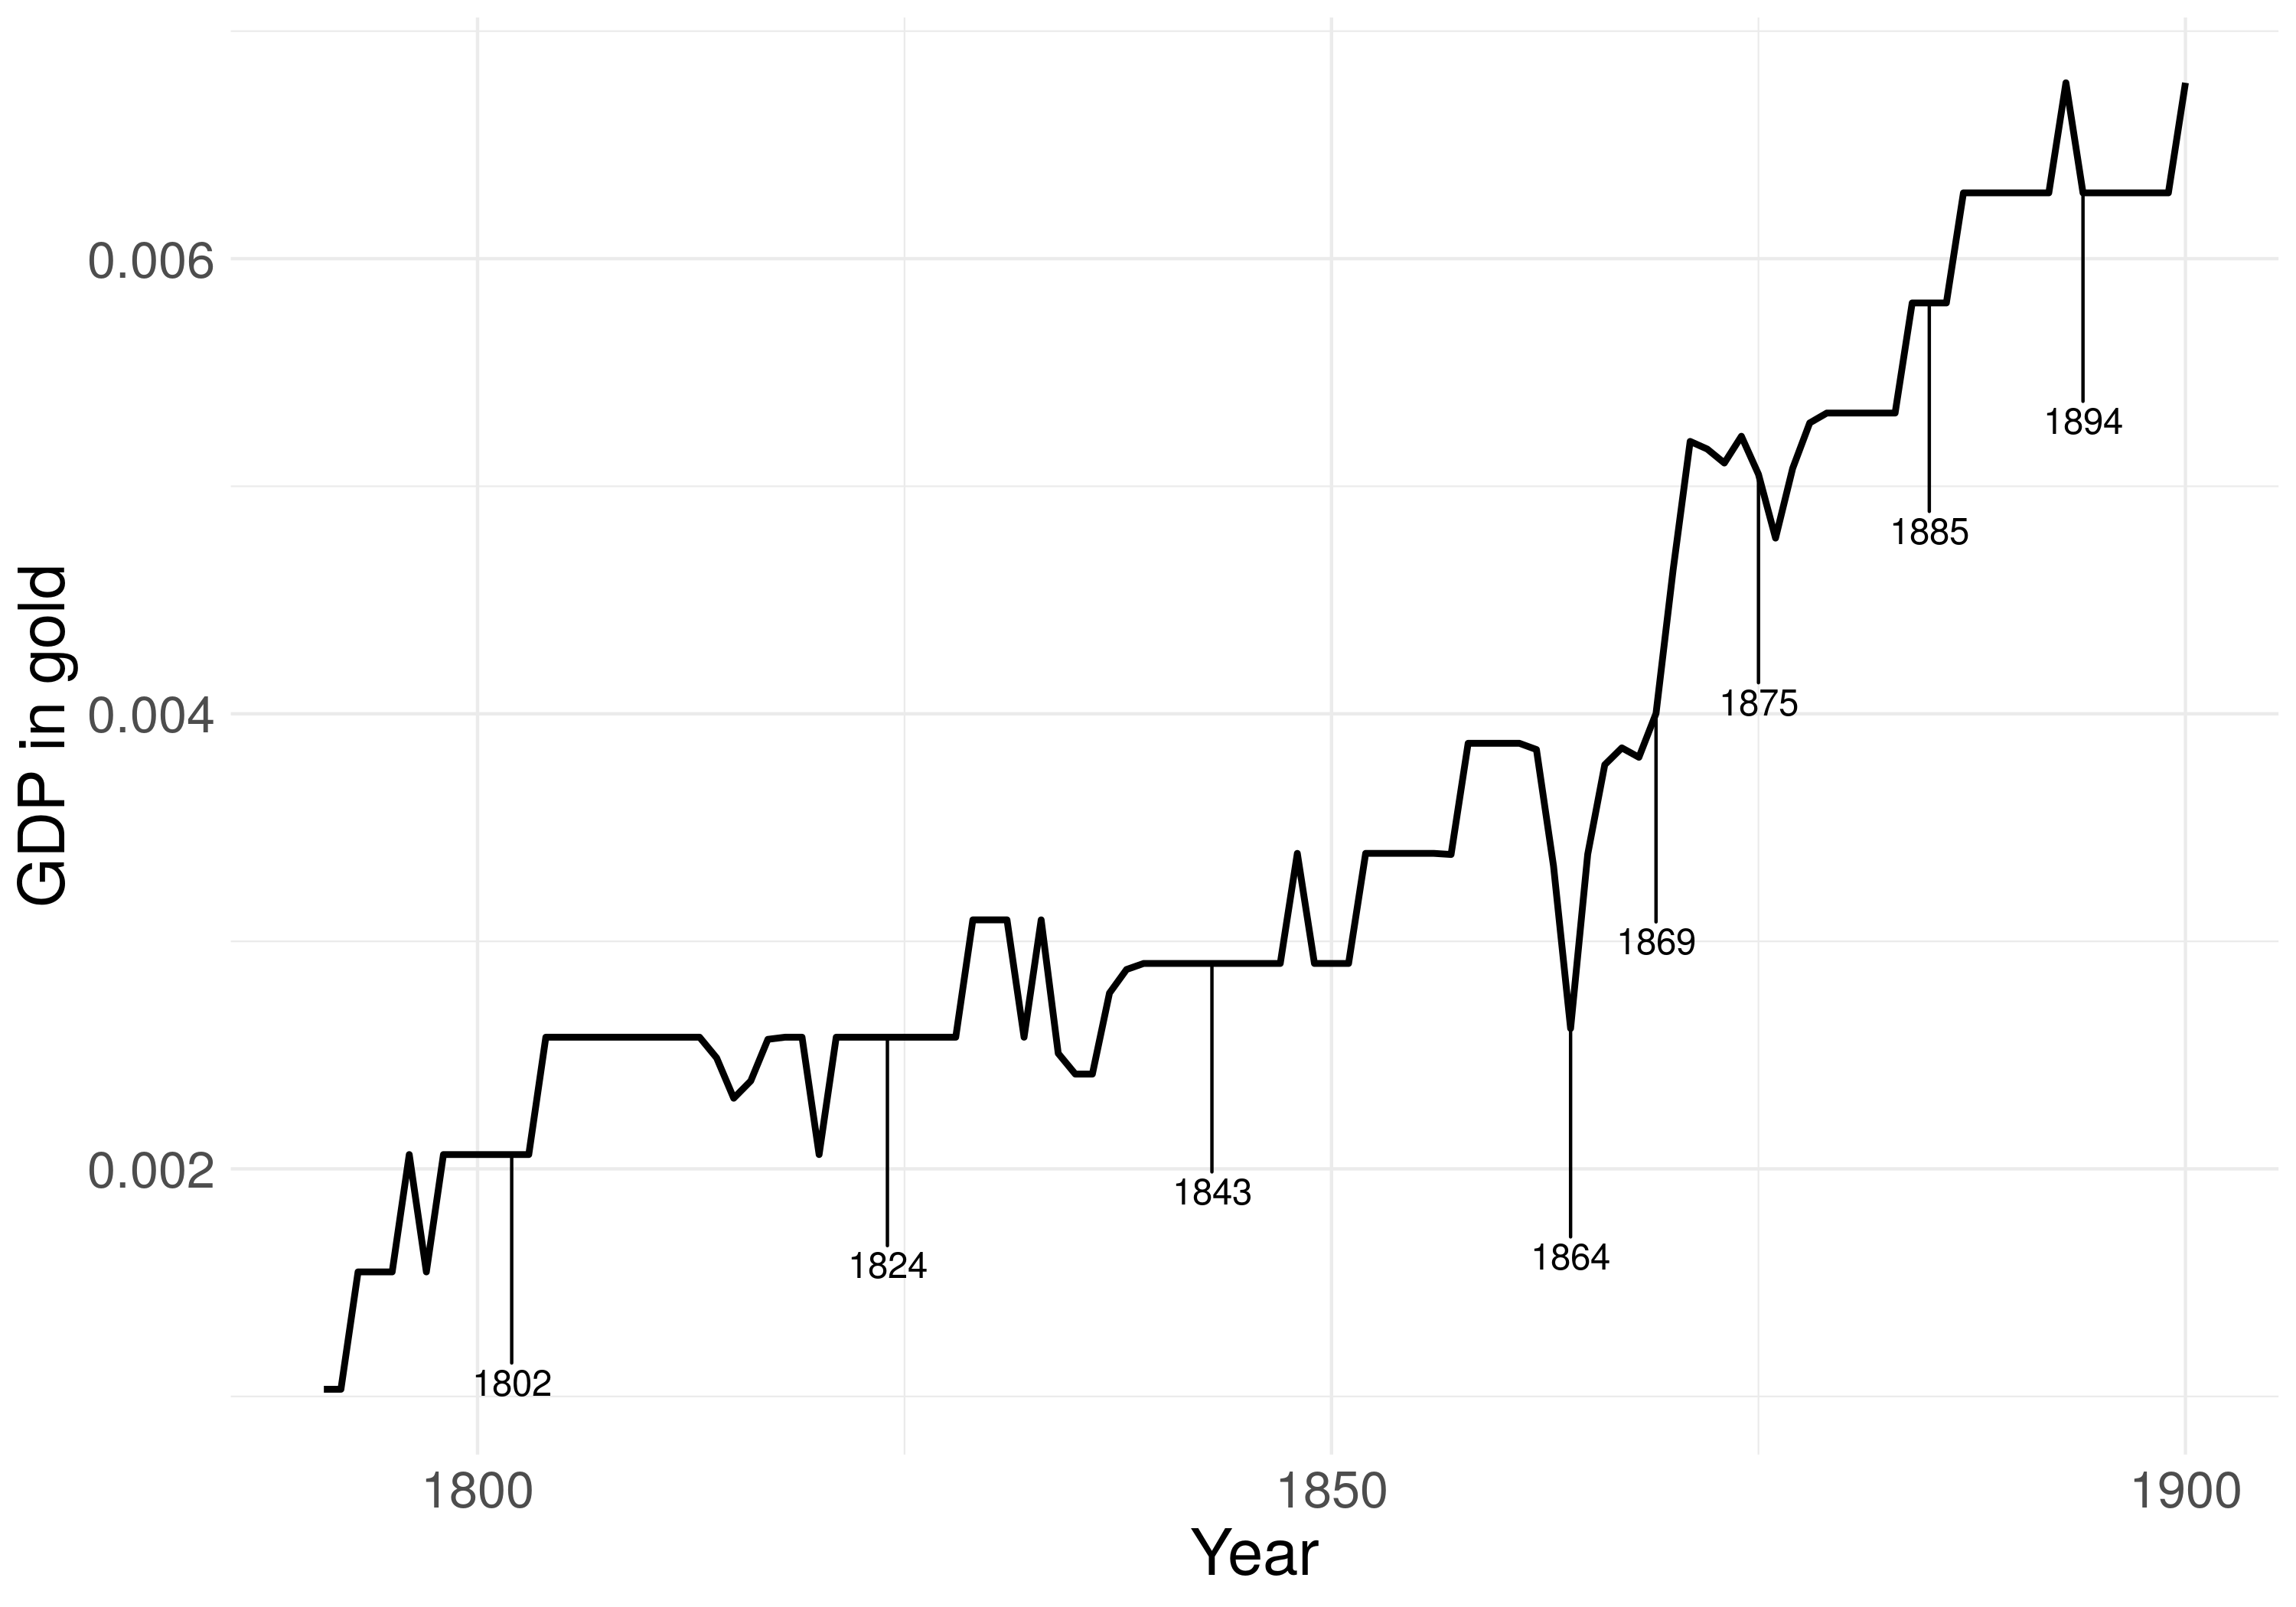
\includegraphics[width=0.75\linewidth]{wage_us_complement.PNG}
			\label{fig:salario_us_comp}}
		\caption{GDP and Wage. US. 1791-1900} \label{fig:us_complement}
	\end{figure}
	
	 
	 Also for completeness, in figure \ref{fig:uk_gdp_complement} we show the UK GDP between 1900-2017. There we highlight the same periods as in figure \ref{fig:series_crisis}. We can recognize a similar pattern to the ones in US, with the difference that the growth between 1940-1975 is slower, and the growth after the eighties seems to be higher. 
	 
	 \begin{figure}[H]
	 	\centering
	 	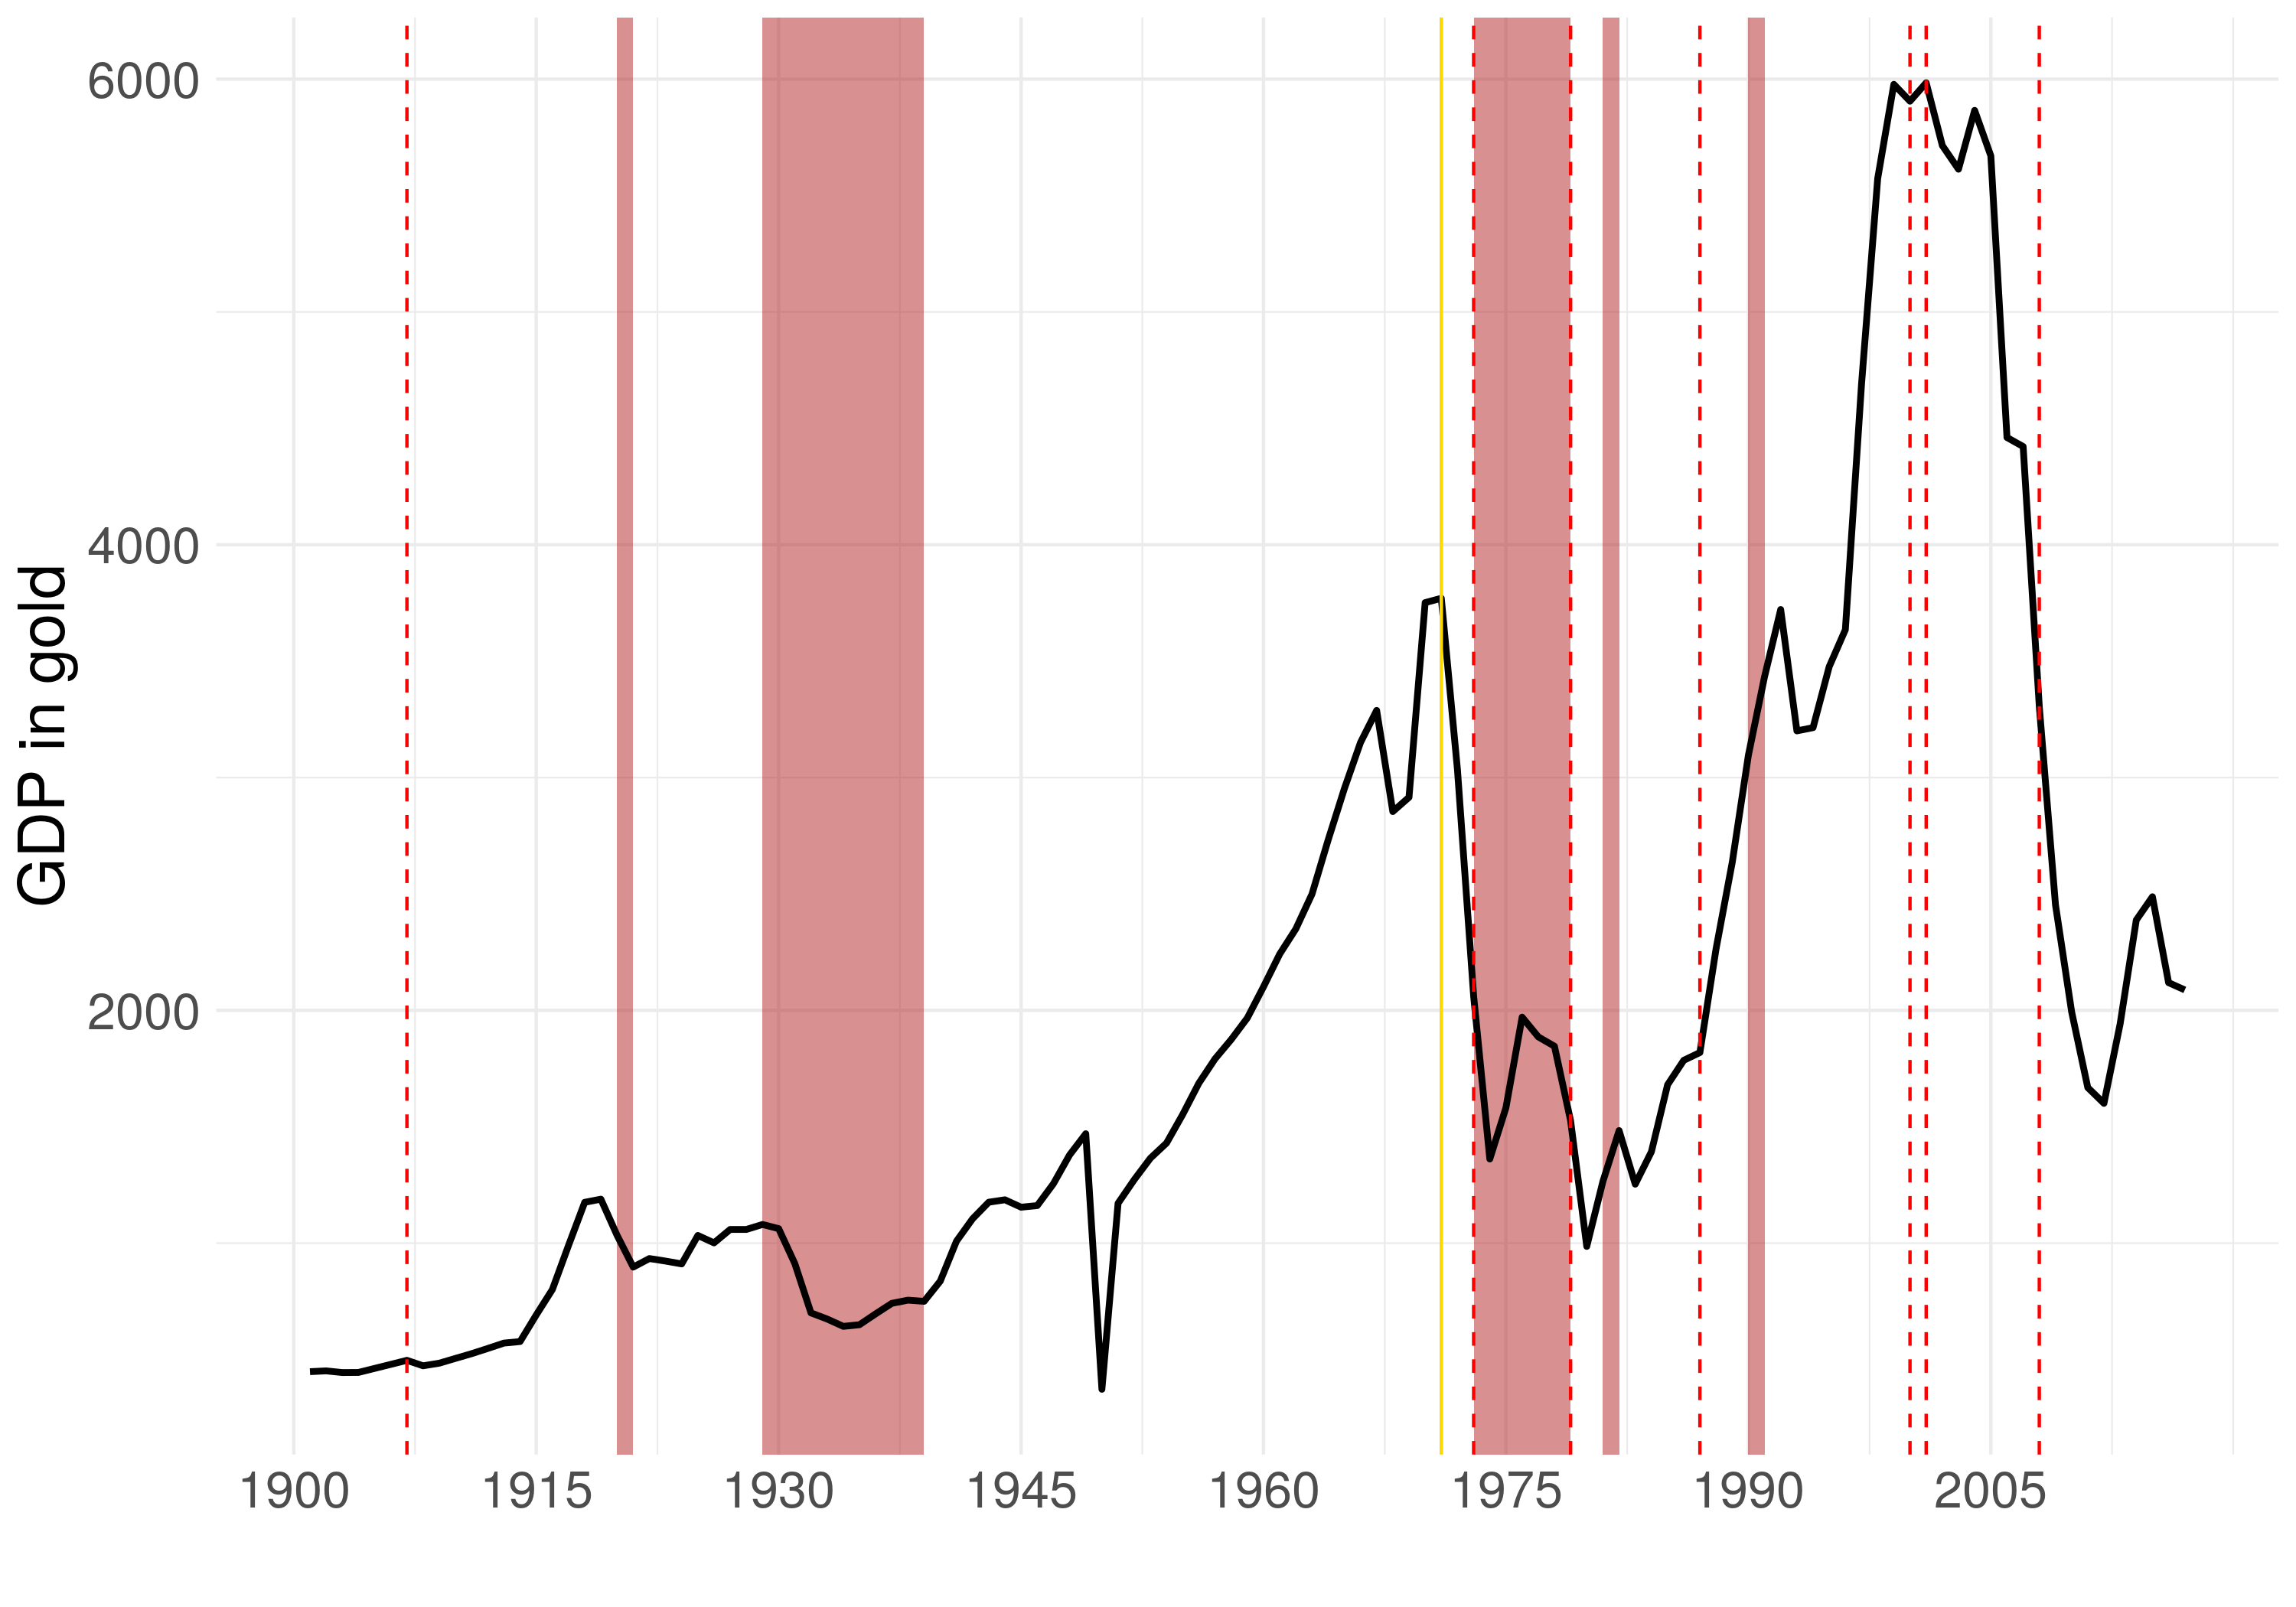
\includegraphics[width=0.75\linewidth]{gdp_uk_complement.png}
	 	\caption{UK GDP. Millions of ounces of gold. 1700-1900} 
	 	\label{fig:uk_gdp_complement}
	 \end{figure}
	 
	 	
	Finally, for comparison, we show the Maddison Project \citep{bolt2014} data for the global GDP per capita. Unfortunately this information has only yearly data starting in 1950, and so cannot be used in the wavelet analysis. In figure \ref{fig:global_gdp} we can see that the aggregated data to a global scale does not how the same fluctuations that we could see on UK and US data, that also had a correspondence with the literature about the main crisis during the twentieth century. For this, we consider that the best available information for the following analysis is the GDP in terms of gold, both for UK and US in the defined periods. 	

	 \begin{figure}[H]
		\centering
		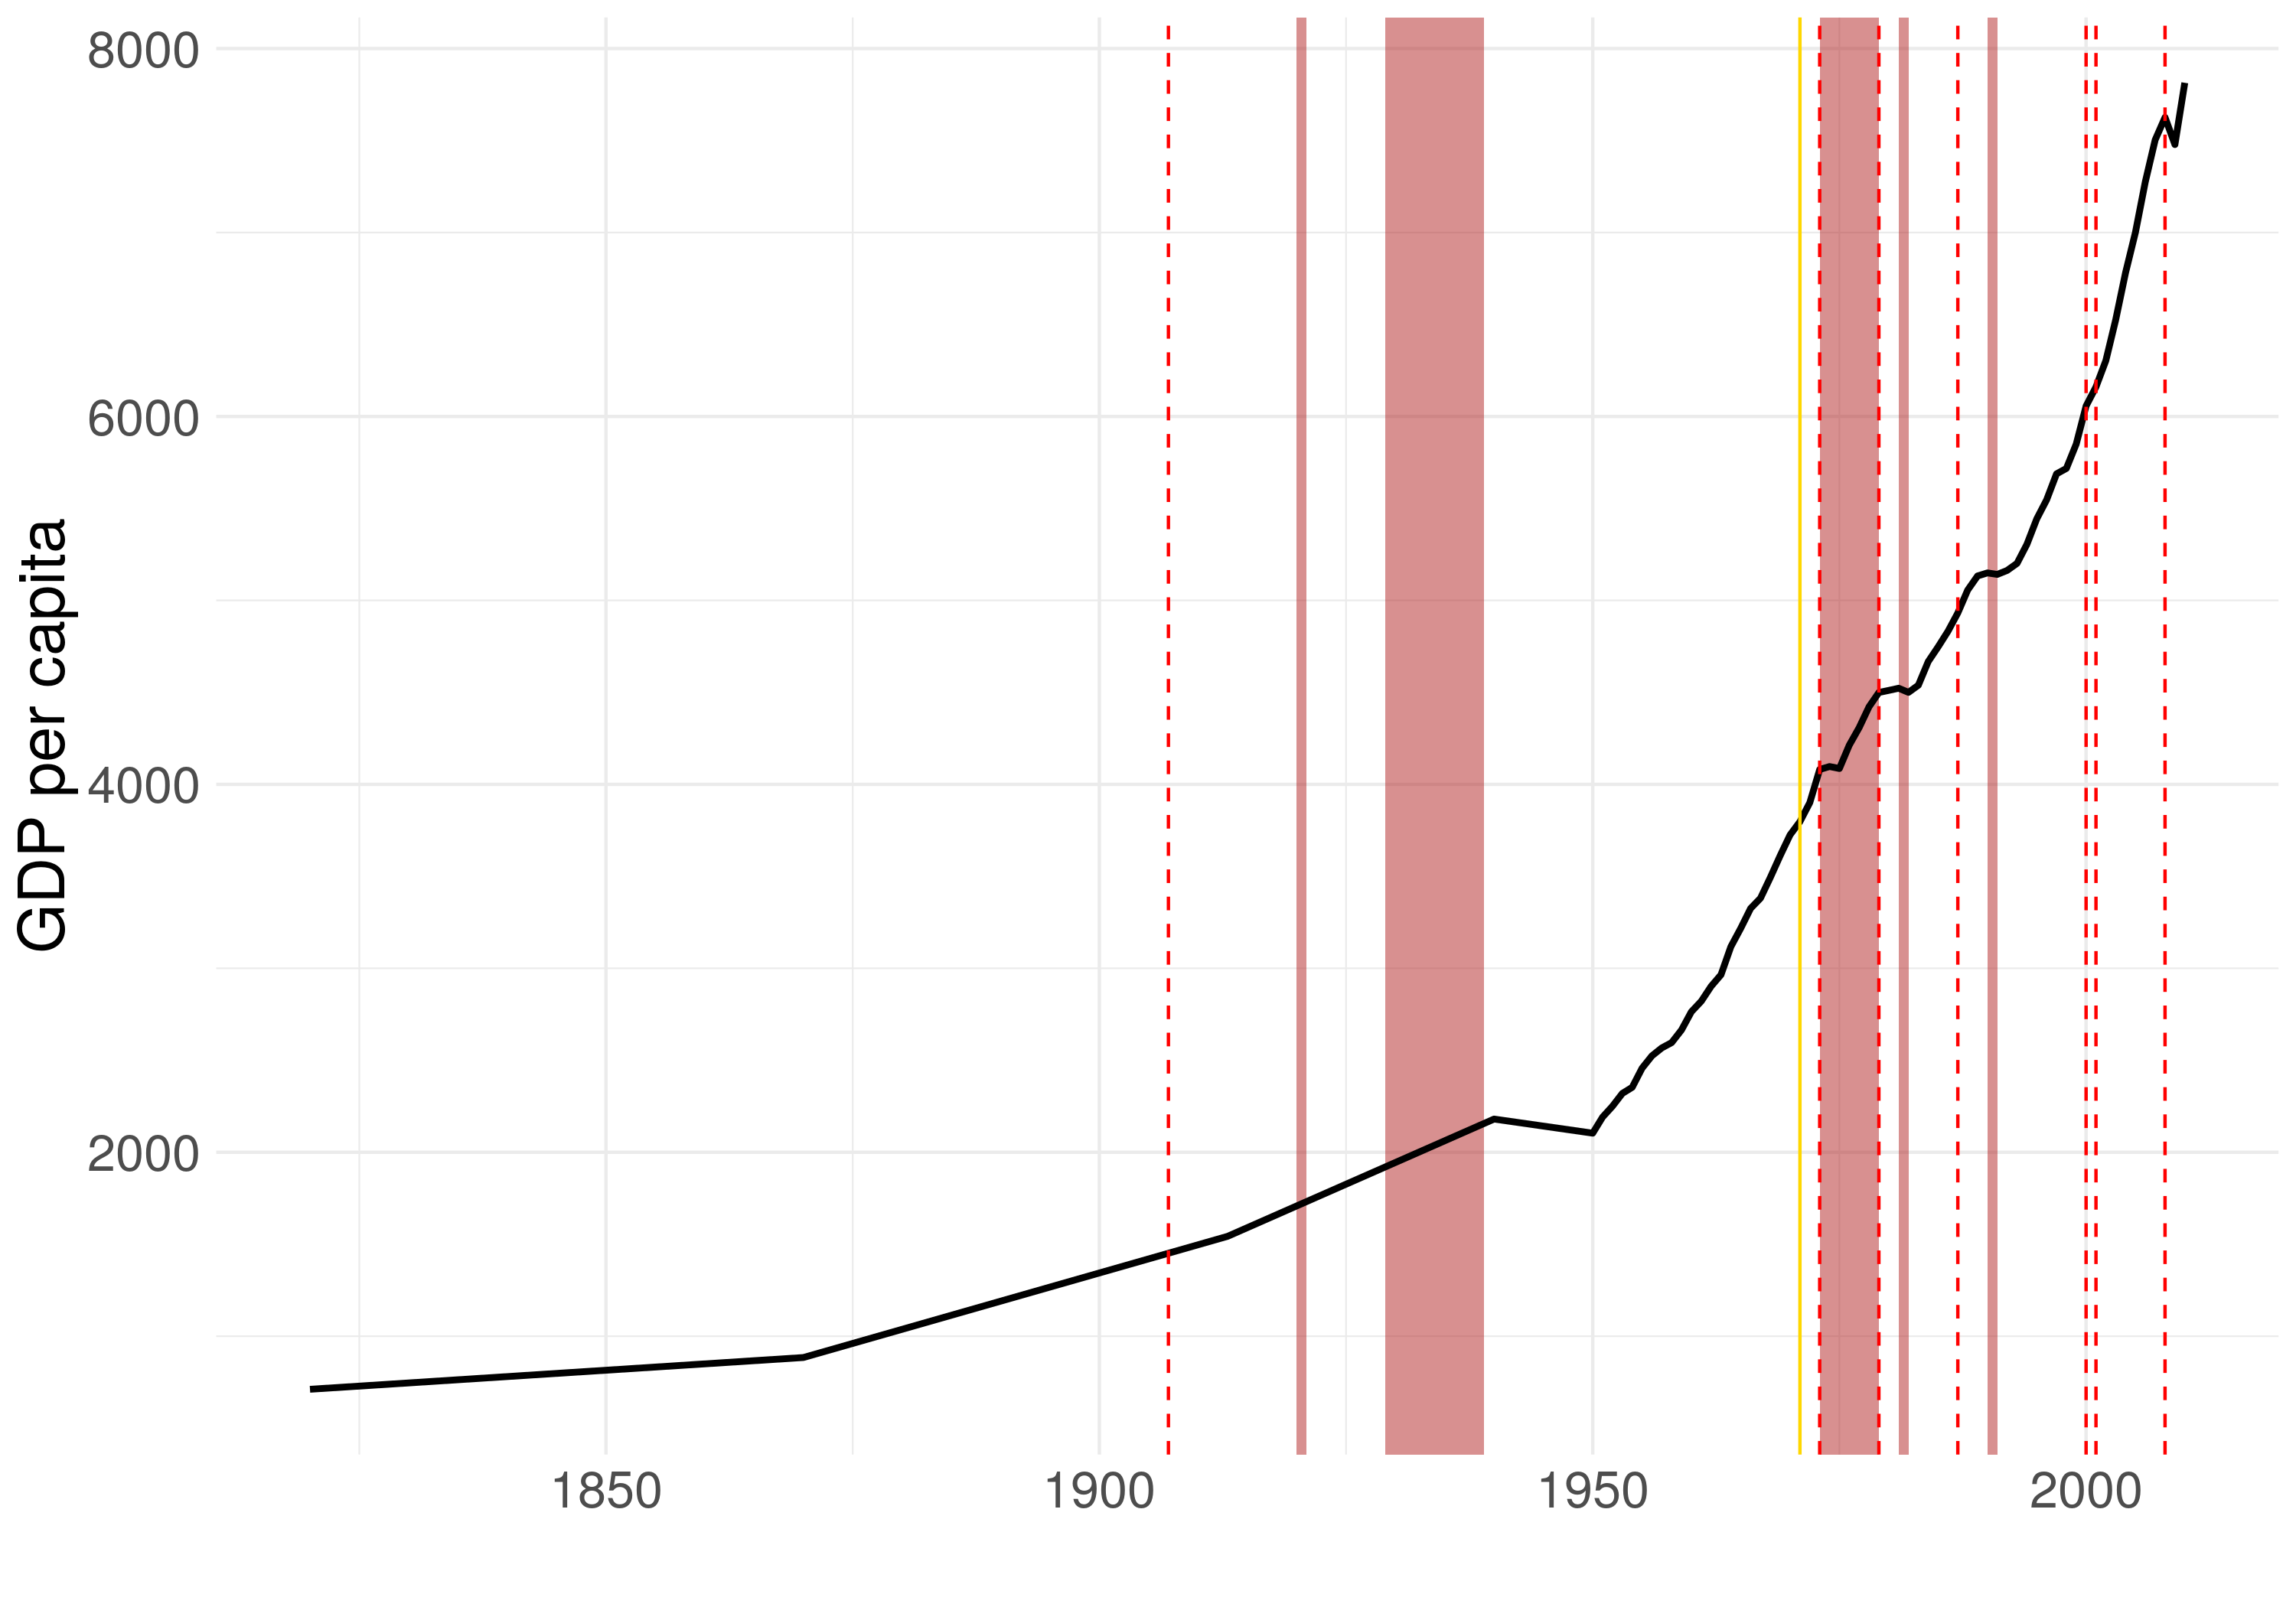
\includegraphics[width=0.75\linewidth]{global_gdp.png}
		\caption{Global GDP per capita. 1820-2010} 
		\label{fig:global_gdp}
	\end{figure}
	
	
	In the following section, we will use the described series will as inputs for a technique coming from the field of signal processing, Wavelets, which allows automatic highlighting of the essential cyclic amplitudes of the series.
	
	\section{\uppercase{\textbf{\normalsize{Wavelets}}}}
	
	Although in econometrics the use of autoregressive models and moving averages for the analysis of time series is extended, there are other widely disseminated techniques in the literature of signal analysis that is not yet extensively used in the study of economic series. A classic example in this sense is the Fourier series. This technique analyzes how any time series can is a composition of periodic functions, that is, as the sum of sines and cosines. In this way, we can construct a space of \textit{frequency} ($1/period$) where we define the periodic functions according to their frequency (or extension in time, horizontal movement) and amplitude (vertical movement). Figure \ref{fig:ciclo} exemplify these definitions.
	
	
	\begin{figure}[H]
		\centering
		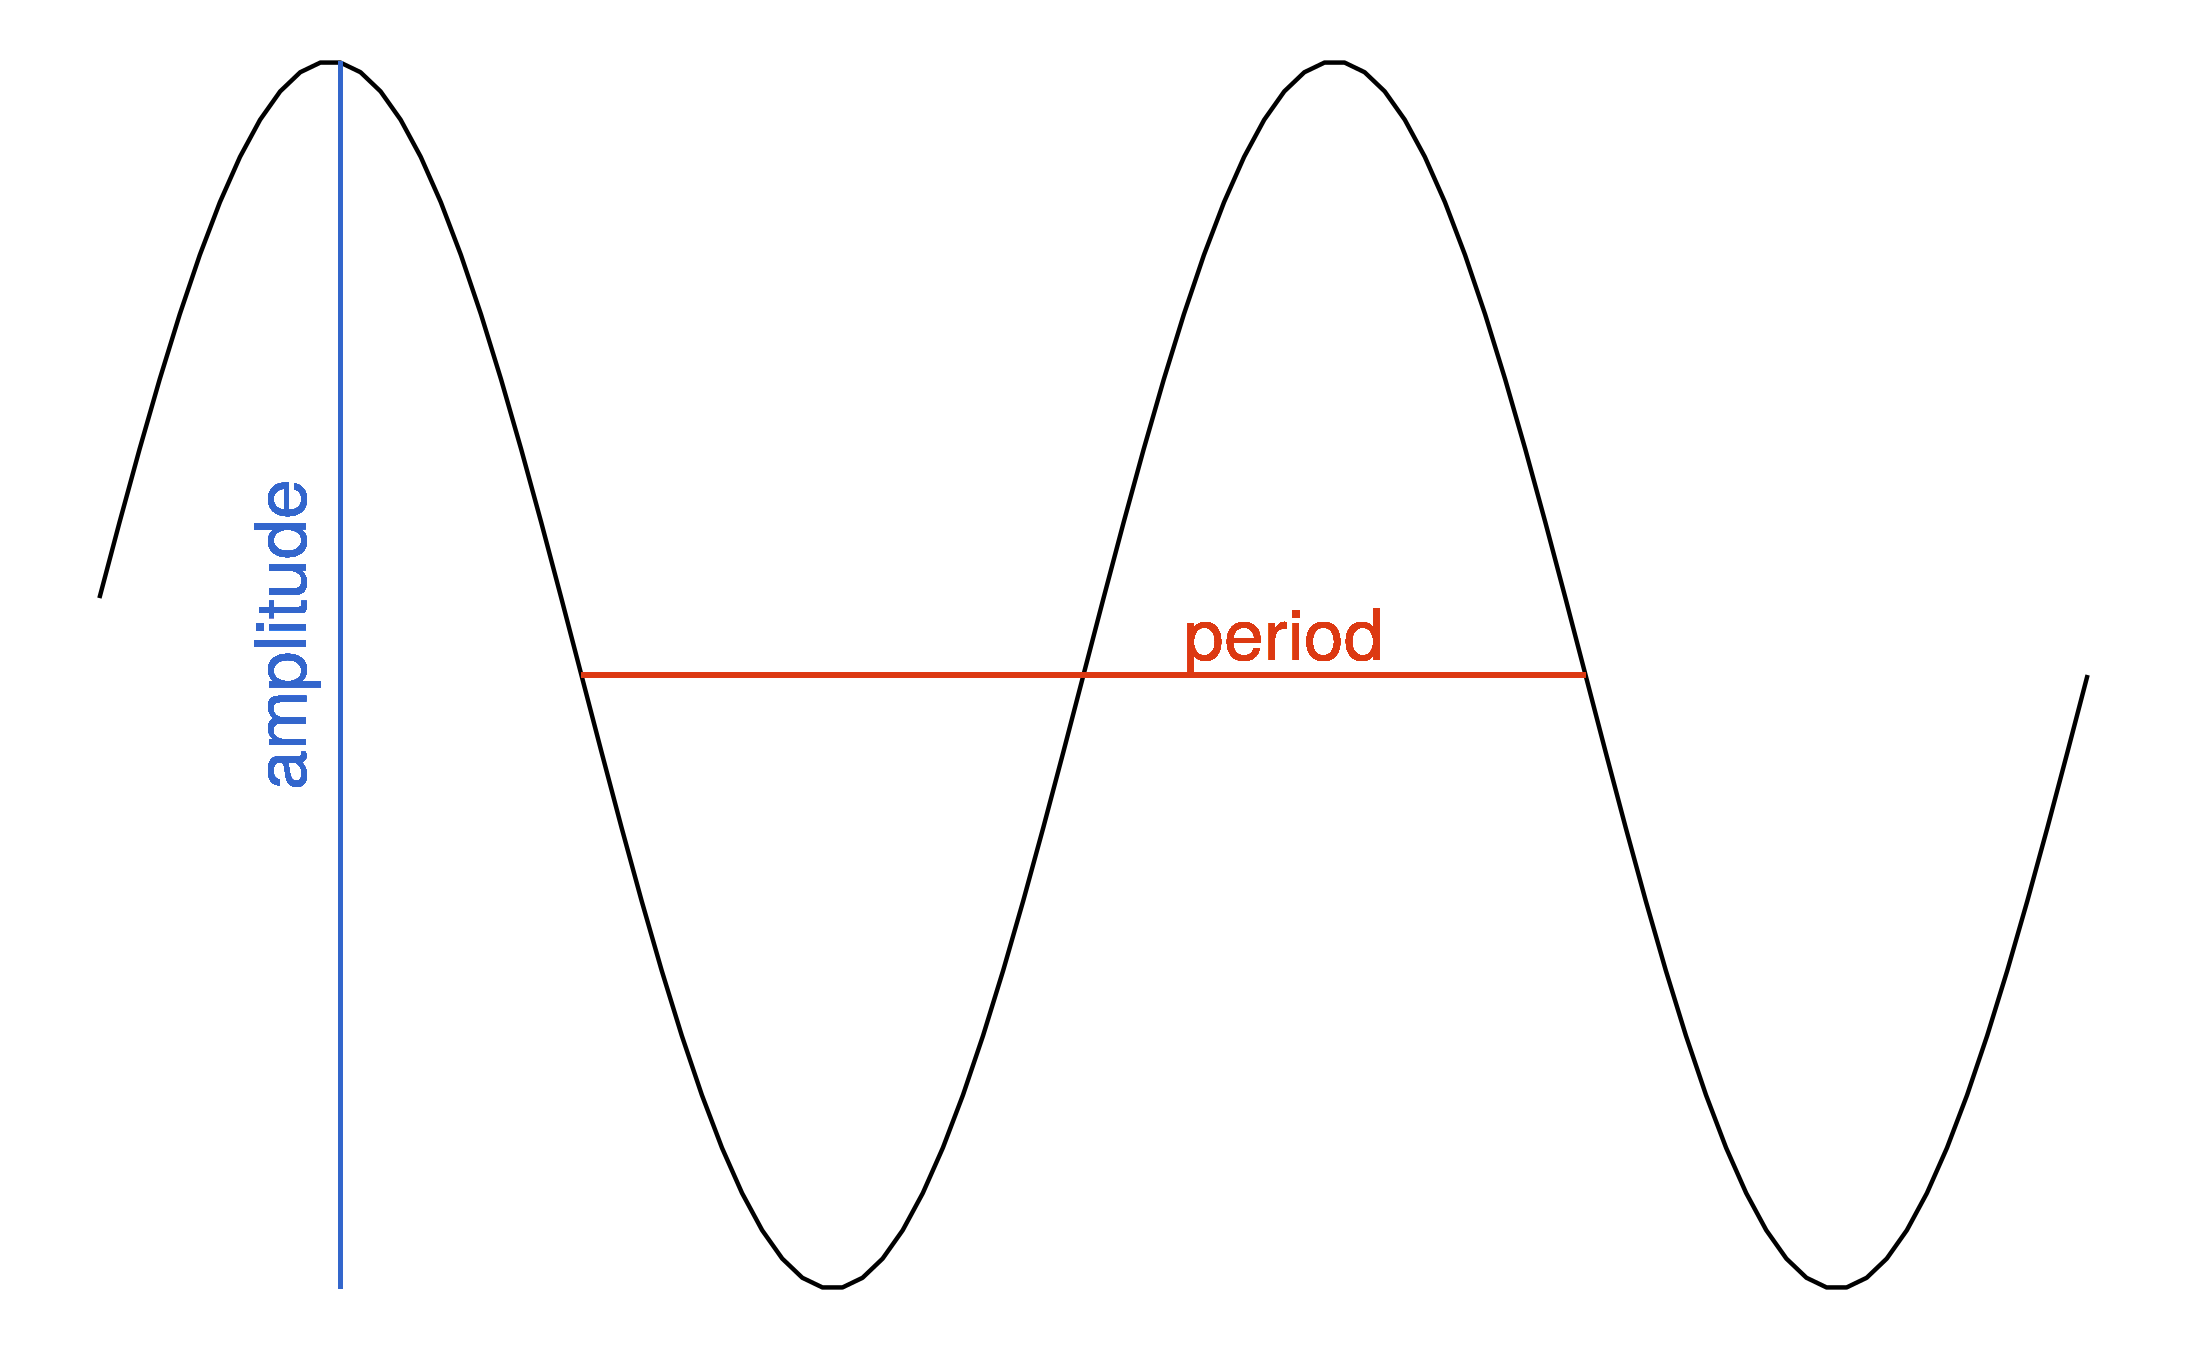
\includegraphics[width=0.65\linewidth]{ciclo_en.png}
		\caption{period and amplitude} \label{fig:ciclo}
	\end{figure}
	
	The base of the Fourier decomposition is the transformation of the domain of series, from the time domain to the frequency domain.
	\\
	
	We can think that the wavelets are also a rotation of a space of functions to a different domain, i.e., a transformation on the original series. However, unlike the Fourier transform that has sines and cosines as the basis of functions, the Wavelet transform has a particular type of base function, called \textit{Wavelets} \cite{castro1995wavelets}. We construct a base of this type from a mother function, which is a short wave, of finite duration. That its to say, unlike the sine and cosine functions that extend infinitely across the domain, the wavelets have \textit{compact support}, this means that they use as base functions that do not extend infinitely in the time domain. Another characteristic of wavelet functions is that the area under the curve must be zero, it has its center at zero. This mother function moves and dilates to build an orthonormal basis.
	
	Whereas a Fourier transformation of a series from the time domain to the domain of the \textit{frequency} takes the form of:
	
	$$
	X(F)=\int_{-\infty}^{\infty} x(t) e^{-j2\pi Ft}dt
	$$
	
	The wavelet transform goes from the domain of time to the domain of \textit{scale} and \textit{translation}:
	
	$$
	X(a,b)=\int_{-\infty}^{\infty} x(t) \psi^*_{a,b}(t)dt
	$$
	
	The scale describes the frequency (inverse of the extension or period) of the cycle, while the translation describes the movement along the series. Since low-frequency series (longer cycles) occupy a more significant portion of the series, they are harder to locate at a particular moment in time. For the above, the resolution in low frequencies is low in the time domain, but good in the frequency domain, while the high-frequency cycles have high resolution in the time domain, but less resolution in the domain frequency domain. If we compare it with the Fourier transforms, we might think that it has very high resolution in the frequency domain, but no resolution in the time domain. The wavelet manages to define the presence of a particular frequency in a specific moment.
	
	It is also possible to understand wavelets as a correlation analysis between a time series, and some compact wave function at one point of time and a particular frequency. The translations generate a shift of the wave function, and therefore we can calculate the correlation for the entire time range. Rescaling modifies the frequency of the wave function, which allows calculating the correlation for several different wave frequencies. The amount of available data is what defines the ability to rescale the base function. That is, how low are the minimum frequencies that can be analyzed. Finally, what we obtain is a value of the linear association between the original series and the base function, for each value of time and frequency.
	
	The base function we use for the present work is called \textit{Morlet Wavelet}, which as implemented in the WaveletComp \citep{Roesch2018} library has the following functional form:
	
	$$
	\psi(t)=\pi^{-\frac{1}{4}}e^{i\omega t}e^{\frac{-t^2}{2}}
	$$
	
	
	Where $\omega$ is the angular frequency (rotation rate in radians per unit of time). This is a continuous, complex function, frequently used in the literature \citep{conraria2011continuous}. The base from the translation, $a$, and the scaling, $b$, implemented is:
	
	$$
	X(a,b)=\sum_{t} x(t)   \frac{1}{b} \psi^*\left(\frac{t-a}{b}\right)dt
	$$
	
	Visually, we can see the translations and rescaling of the base function in the figure \ref{fig:morlet}. There the translations are defined in the time domain, while rescaled do in the frequency domain. If we reconstruct the time-frequency plane and calculate the correlation of each point with the original series, a new dimension is obtained that represents the degree of adjustment of our series at each frequency, for the different moments.
	
	\begin{figure}[H]
		\centering
		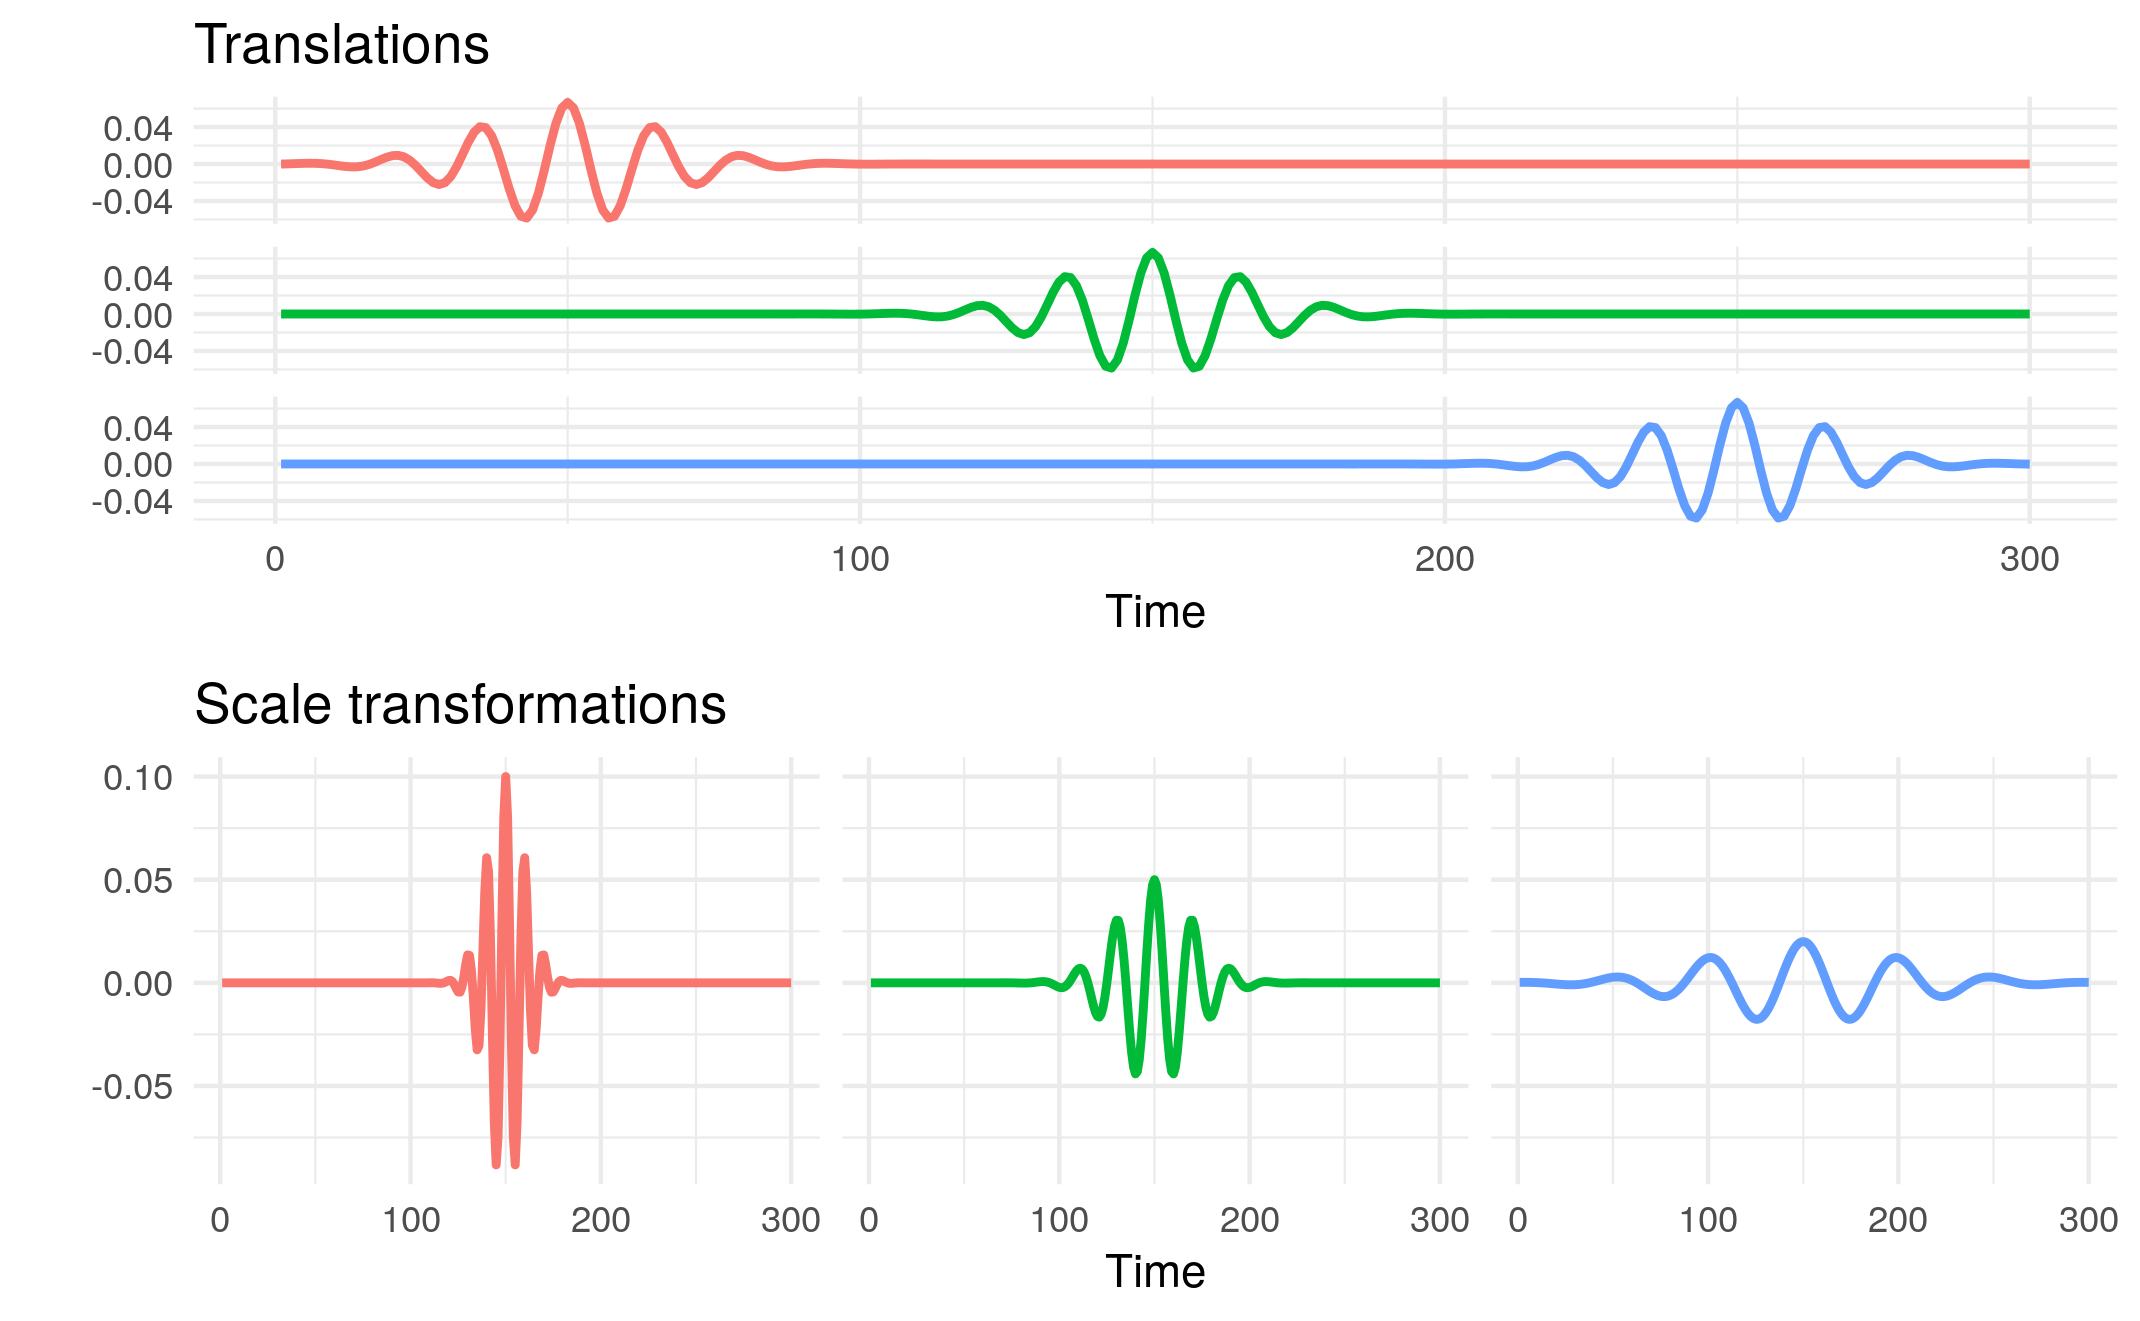
\includegraphics[width=\linewidth]{morelt_en.png}
		\caption{Translation and rescaling of the Morlet base function} \label{fig:morlet}
	\end{figure}
	
	Finally, we can display the results on a \textit{spectrogram}, i.e., for each frequency at each moment the degree of correlation of the original series with Morlett function.
	
	
	It is useful to define a theoretical model of a cyclical economy, with the different components seen separately and in their composition in order to visualize the wavelets in the analysis of the economic cycle. This way we can observe the characteristics of the spectrogram in this model and then compare it with the real data.
	
	In the figure \ref{fig:serie_teorica} 100 values of the different components with which we will build the series are observed, they are:
	
	
	\begin{itemize}
		
		\item \textbf{impulse}: A series with a constant value of 50 in which a particular period takes the value 100.
		\item \textbf{Trend}: Grows half a point per period.
		\item \textbf{short cycle}: A cycle of small amplitude and extension
		\item \textbf{middle cycle}: A cycle of medium amplitude and extension
		\item \textbf{long cycle}: A cycle of large amplitude and extension
		\item \textbf{noise}: Noise generated from a normal distribution, not significant with respect to the amplitude of the cycles and the slope of the trend.
	\end{itemize}
	
	the R code which generates those series is as follows:
	
	\begin{lstlisting}
	n = 1000
	impulse= c(rep(50,(n/2-1)),100,rep(50,n/2))
	trend = c(1:n)/2
	short = 10 * sin(( 2 * pi/3 ) * c(1:n))
	middle = 20 * sin(( 2 * pi/10) * c(1:n))
	long = 30 * sin(( 2 * pi/50) * c(1:n))
	noise <- rnorm(n)
	composite_series = impulse + trend + short + middle + long + noise
	\end{lstlisting}
	
	
	\begin{figure}[H]
		\centering
		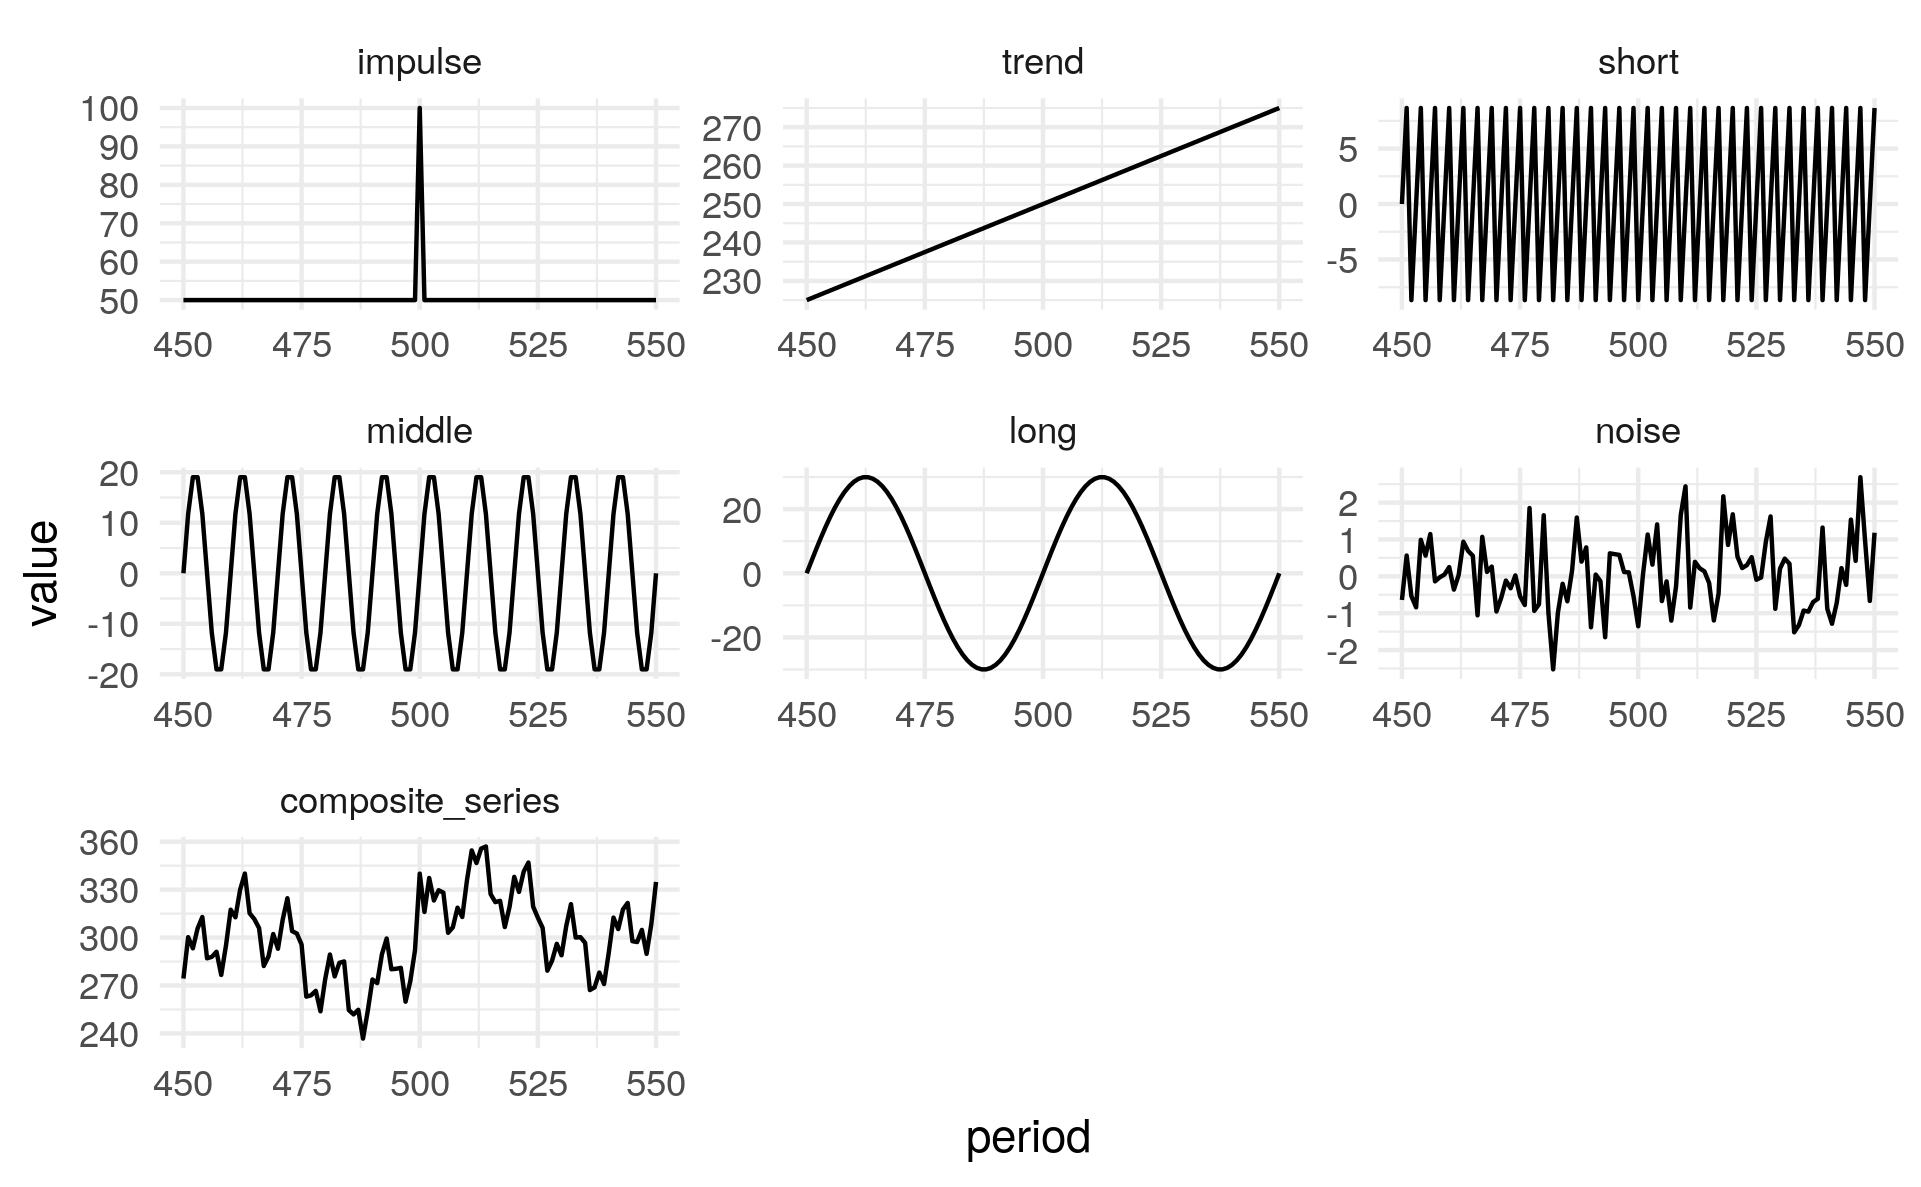
\includegraphics[width=\linewidth]{serie_teorica_en.PNG}
		\caption{Elements of theoretical series} \label{fig:serie_teorica}
	\end{figure}
	
	We can see the spectrogram of each one of the mentioned elements in the figure \ref{fig:espect_teo}. These plots show on the vertical axis the period, the inverse of the wave frequency, which corresponds to the distance between the valleys or peaks of a cycle. The color scale (Blue for the lowest values to red in the highest values) represents the amplitude of the cycle. The horizontal axis represents the calendar time. That is, for each calendar time we can observe the amplitude of the cycle in each of the possible wave frequencies.
	
	
	\begin{figure}[H]
		\centering
		\subfigure[impulse]{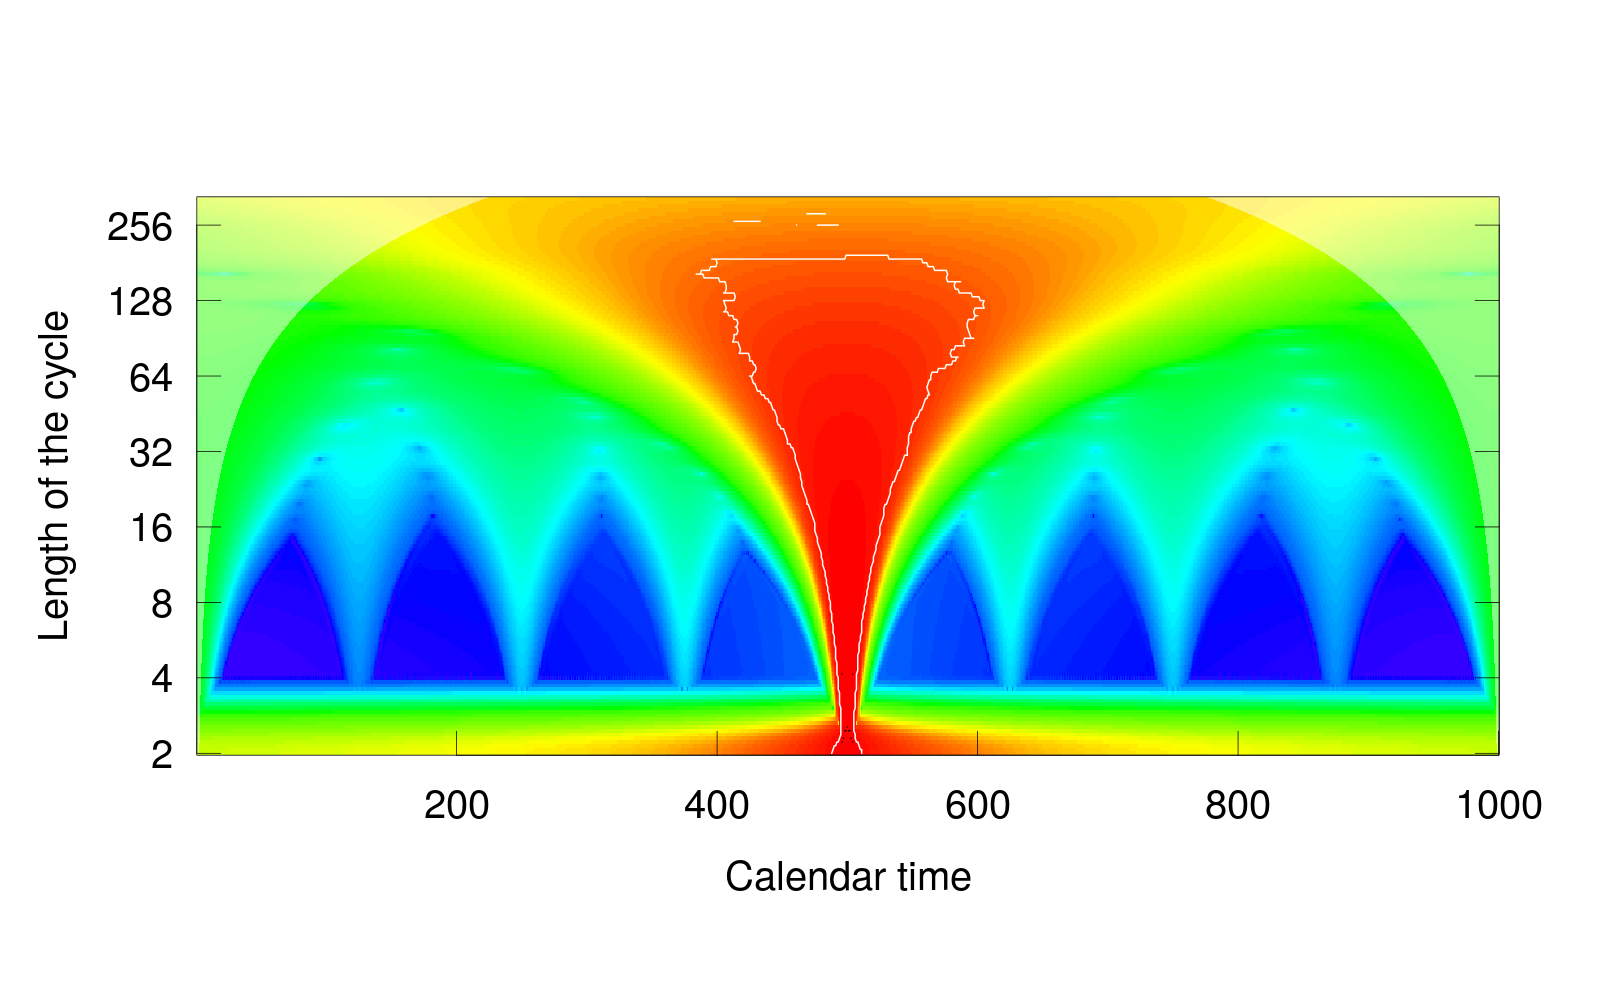
\includegraphics[width=0.49\linewidth]{espectograma_teorico_impulso_en.png}}
		\vspace{0.00mm}
		\subfigure[trend]{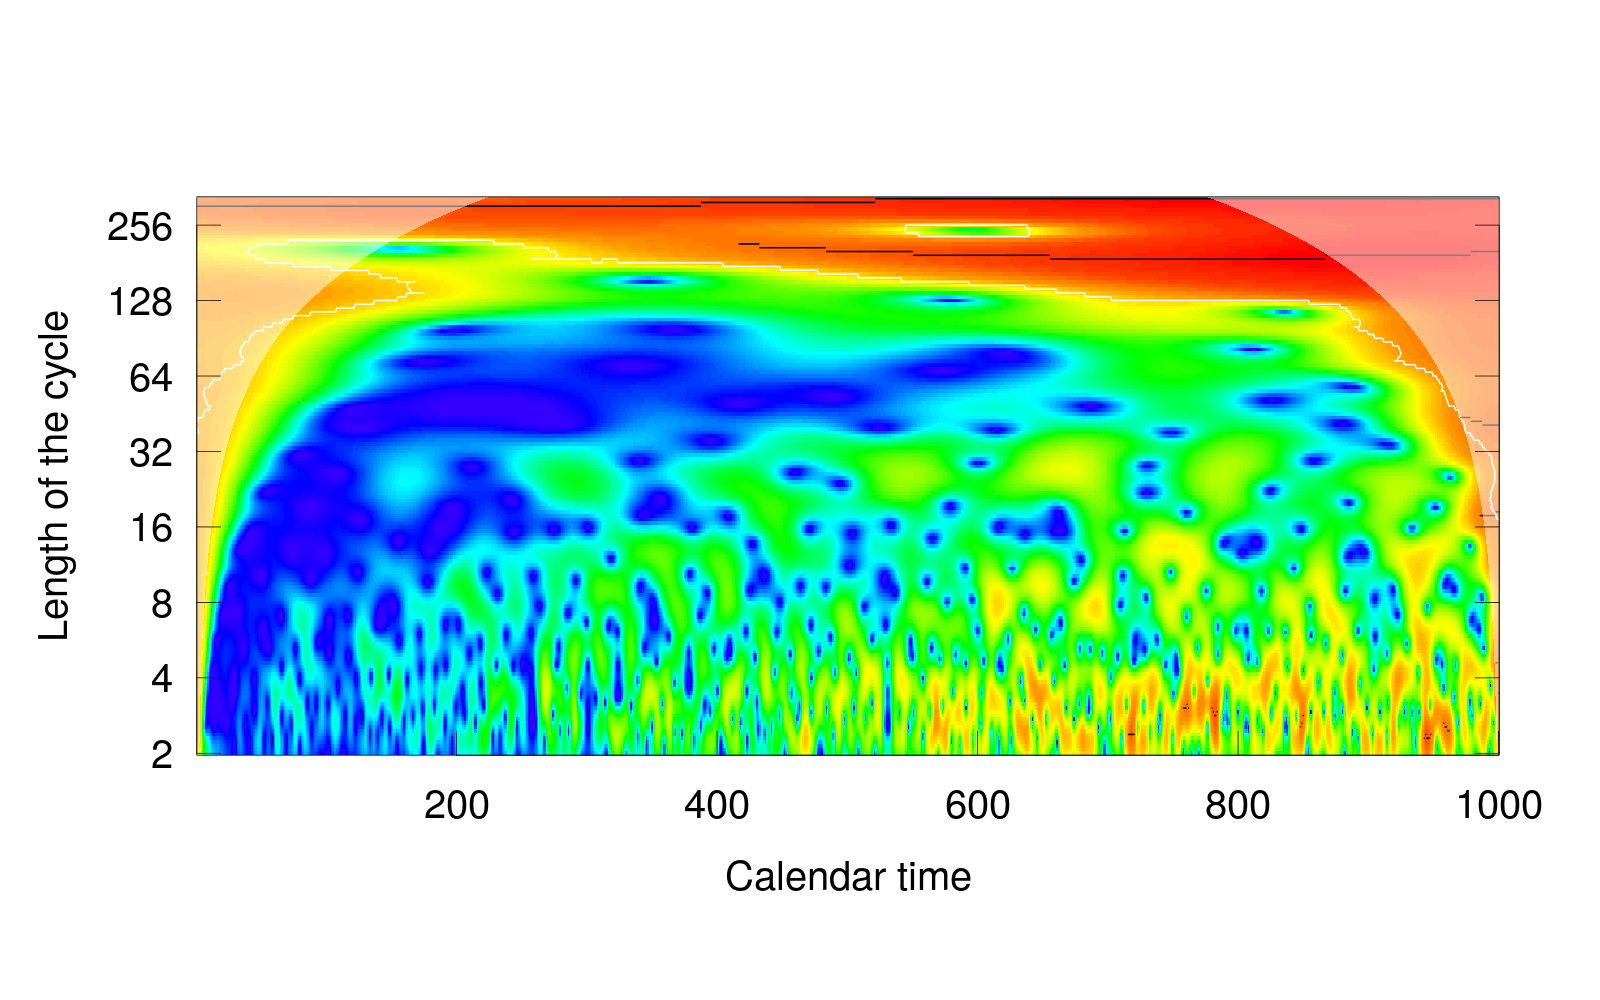
\includegraphics[width=0.49\linewidth]{espectograma_teorico_tendencia_en.png}}
		\vspace{0.00mm}
		\subfigure[3 year cycle]{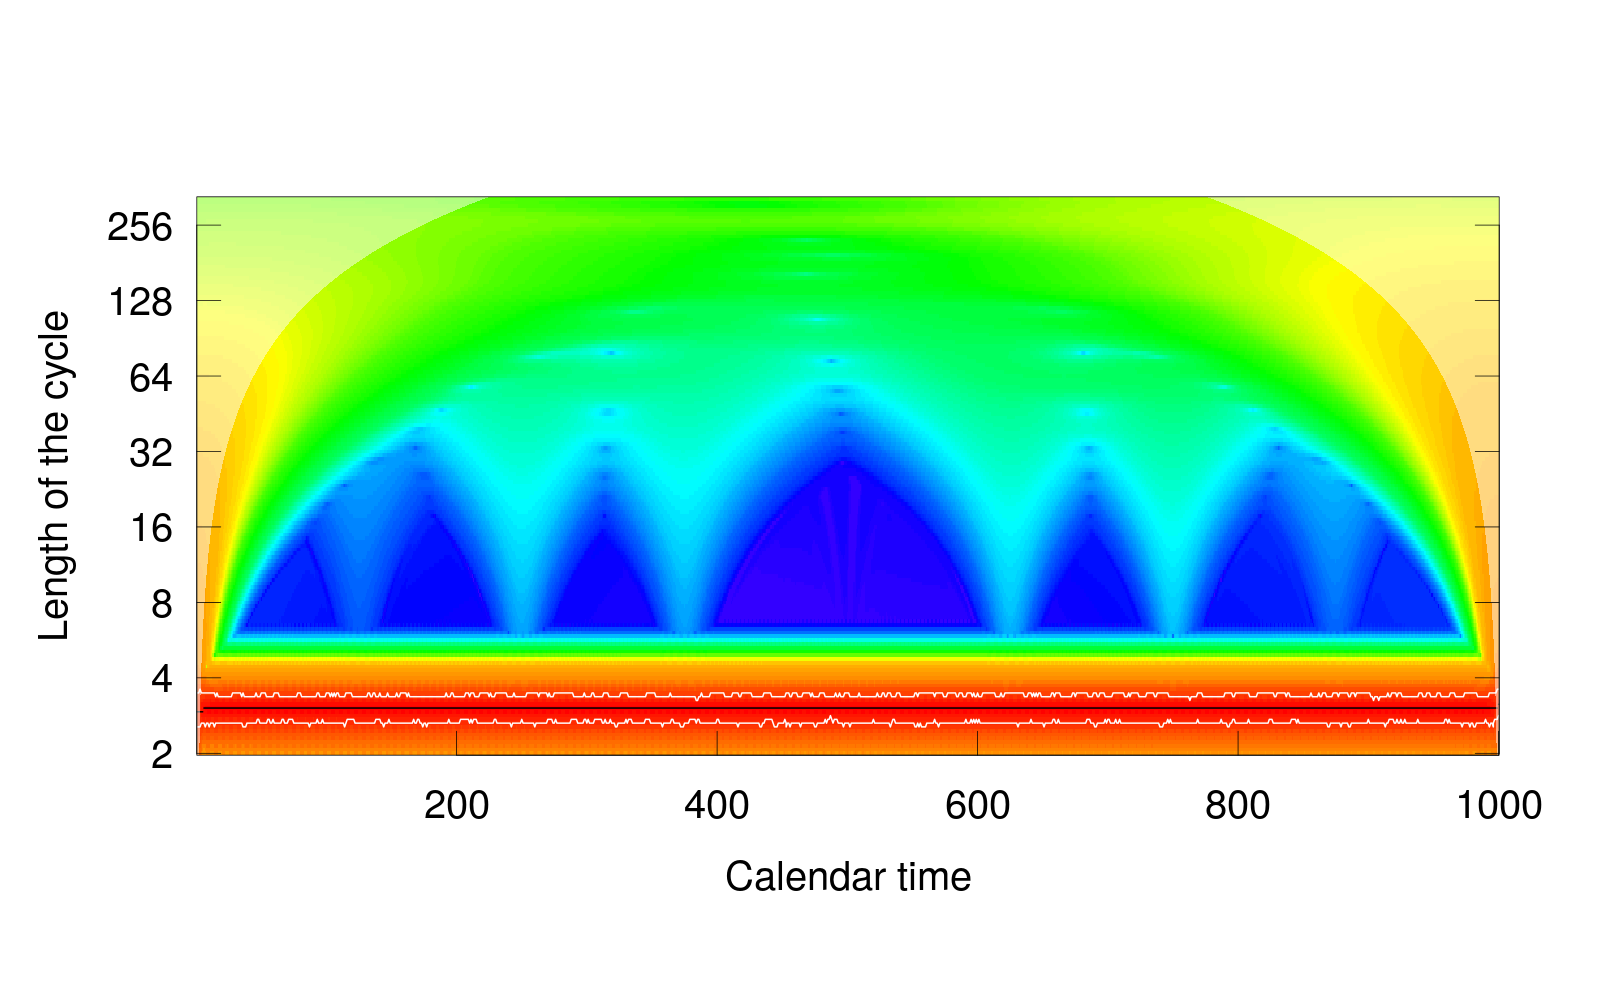
\includegraphics[width=0.49\linewidth]{espectograma_teorico_ciclo_3_en.png}}
		\vspace{0.00mm}
		\subfigure[10 year cycle]{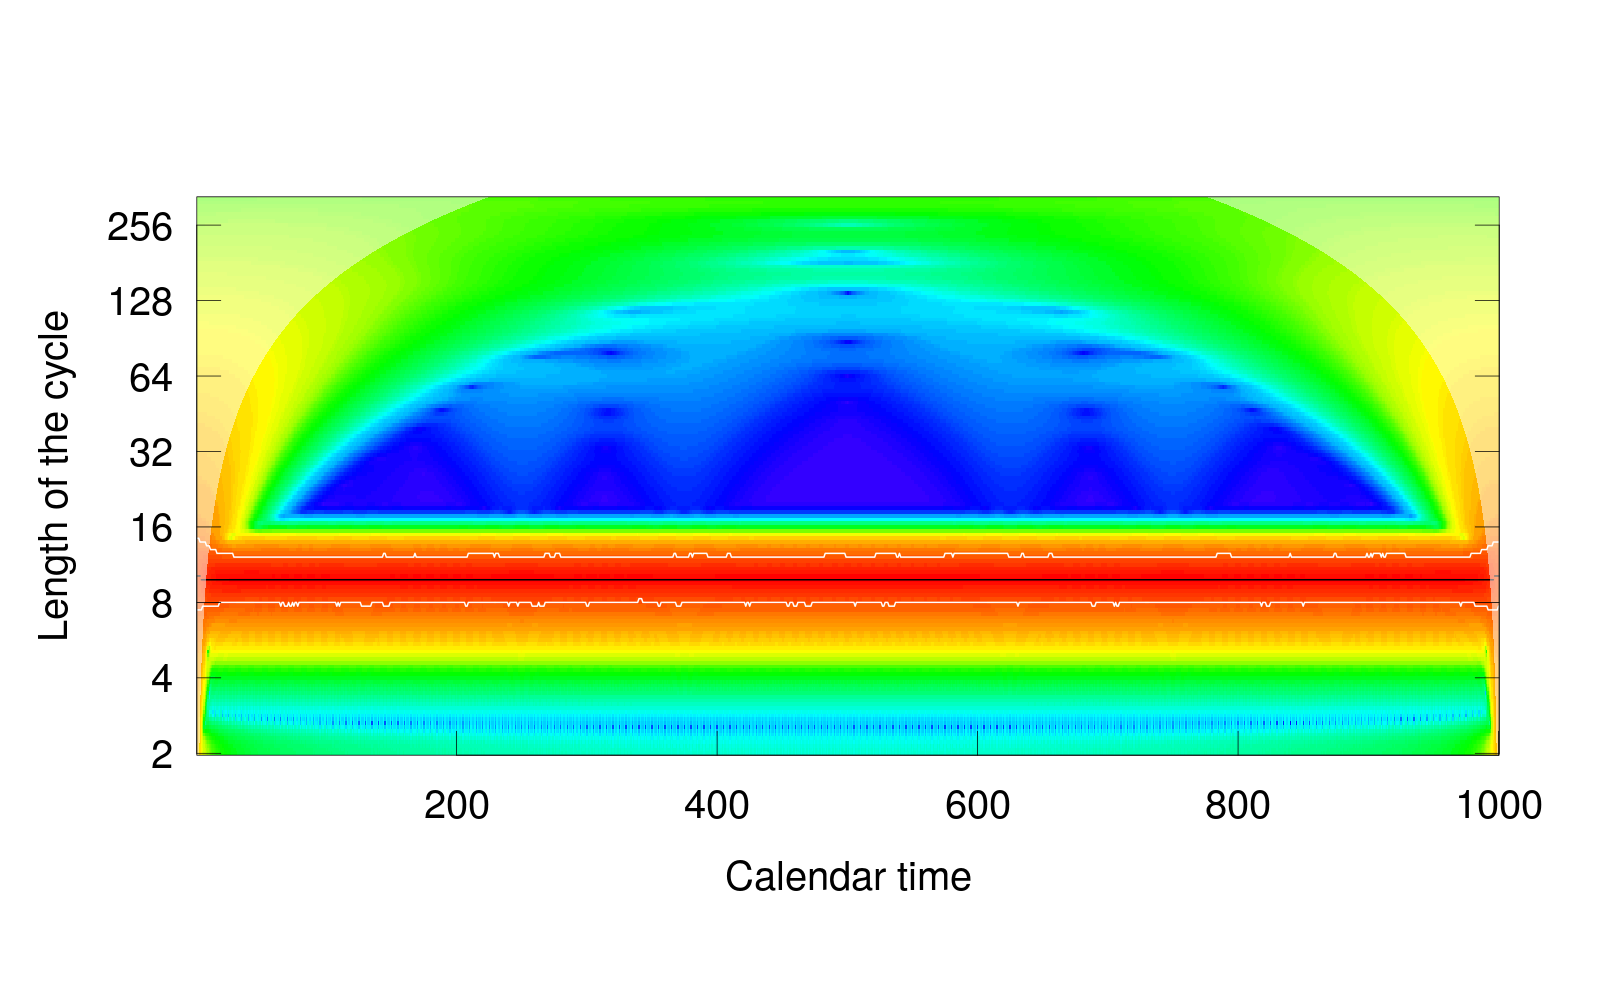
\includegraphics[width=0.49\linewidth]{espectograma_teorico_ciclo_10_en.png}}
		\vspace{0.00mm}
		\subfigure[50 year cycle]{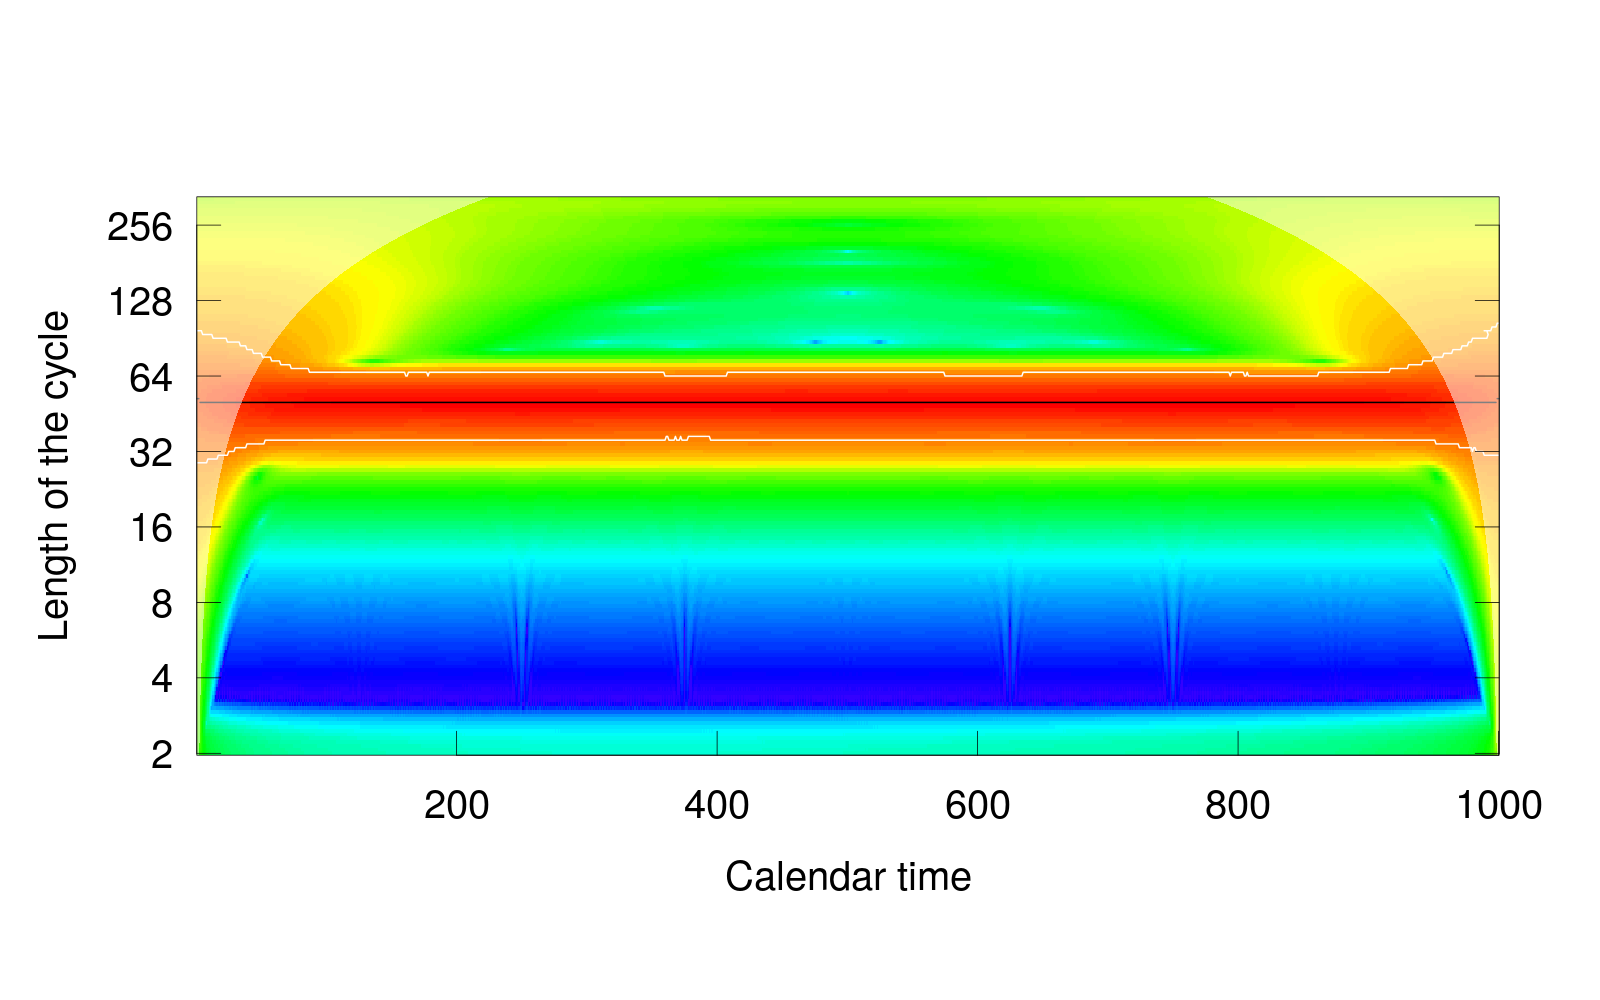
\includegraphics[width=0.49\linewidth]{espectograma_teorico_ciclo_50_en.png}}
		\vspace{0.00mm}
		\subfigure[normal noise]{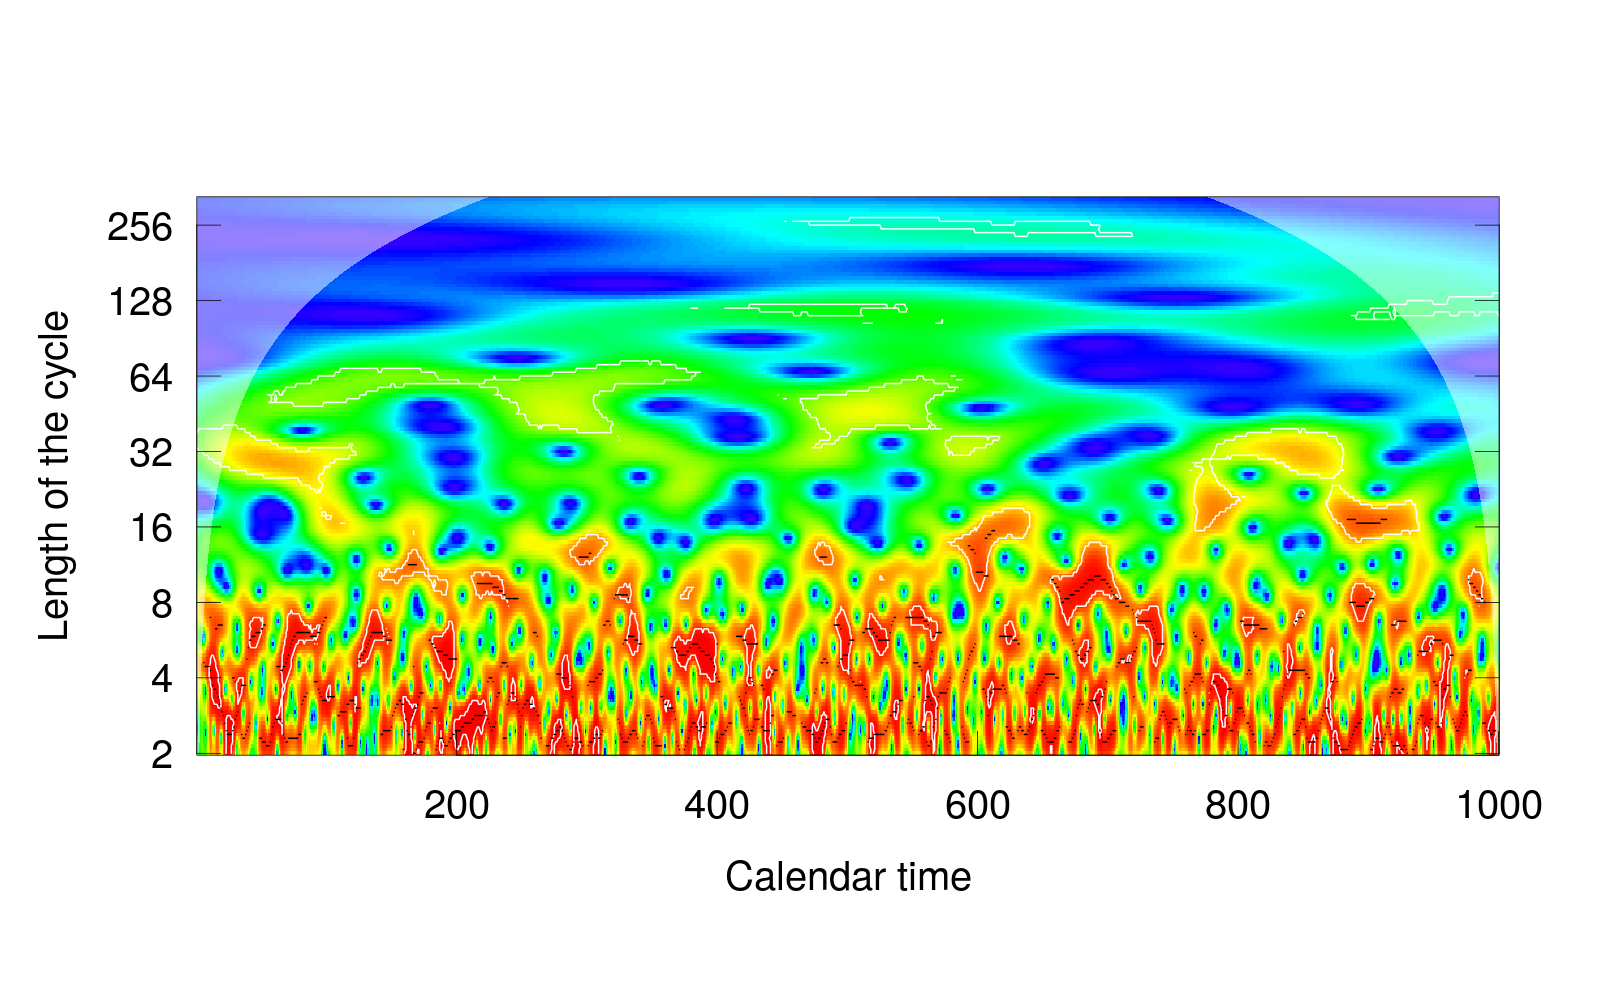
\includegraphics[width=0.49\linewidth]{espectograma_teorico_ruido_en.png}}
		\vspace{0.00mm}
		\subfigure[composite series]{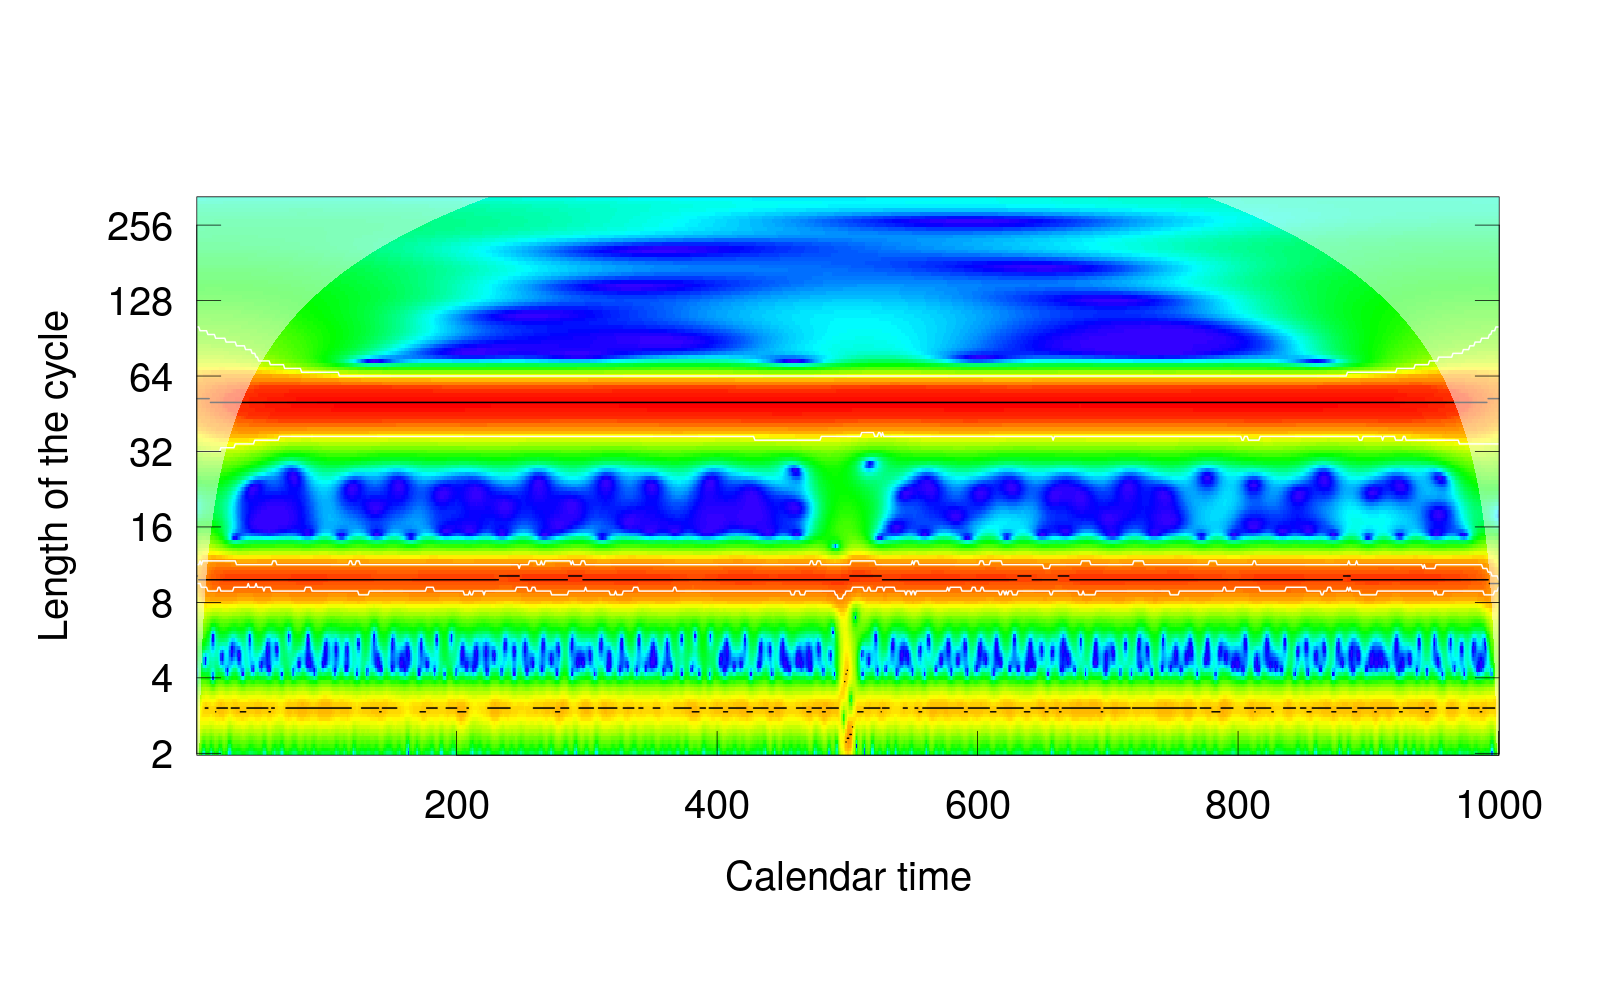
\includegraphics[width=0.75\linewidth]{espectograma_teorico_composicion_series_en.png}}
		\caption{Theoretical spectrograms} \label{fig:espect_teo}
	\end{figure}
	
	As shown in the figure \ref{fig:espect_teo} the impulse is presented as a cycle of large amplitude in all frequencies for the moment corresponding to the jump. The tendency, on the other hand, is primarily shown as noise, given that it is strictly a non-cyclical behavior. Nonetheless, it has the characteristic of taking higher amplitude values towards the end of the period for low frequencies and unusually low amplitude values in the high frequencies of the first moments.
	
	The three defined cycles mark a horizontal line in the corresponding period, which dilutes towards the other frequencies. Finally, normal noise has a very particular behavior, showing greater amplitudes, irregularly, at high frequencies, and homogenizing towards a low amplitude value in longer cycles. This is due to the fact that normal noise can resemble a cycle of very short periods due to a succession of ups and downs, but since it is a random process, it is increasingly unlikely to resemble cycles of more extended periods, given that this would imply a more significant number of successions of consecutive increases and decreases. In turn, both in the spectrogram of normal noise and in that of the trend, it can be seen how the graph loses resolution for more extended periods, as mentioned above.
	
	
	Finally, in the composition of series, it is observed how the cycles of higher amplitude and frequency express in the chromatic scale in a sharper way than the cycles of smaller amplitude and frequency. It is important to note that the agreement between amplitude and frequency is a product of the way in which we build the series since we expect that the prolonged economic cycles will also correspond to movements of greater amplitude.
	
	It is worth mentioning that the choice for the theoretical model of these three levels and cyclical amplitudes is not arbitrary, but corresponds roughly to what is considered by the literature: \cite{kondratieff1979long} studies the long series, about 50 years, while \cite {kuznets1930secular} proposes secular movements between 15 and 25 years. Finally, the Real business cycle \citep{kydland1982time} considers a short cycle.
	
	This preamble on the simulated data was intended to build an intuition on what we should look for on the plots with real data. The wavelet analysis has a strong point on this spectrograms because they allow us to see the most prominent cycles present in our data. The point of this article is, therefore, to bring a new tool, with a new type of graphical representation for economists, in order to bring new light in the analysis of information long studied in the preceding literature.
	
	
	With the analysis from the figure \ref{fig:espect_teo} we can now see the results of the original series. In the figure \ref{fig:espect_PBI_a} the spectrogram corresponding to the GDP of the United States expressed in gold can be observed. There the difference in the series is marked before and after 1900, and in particular, we can see the studied break of the '70s. Nevertheless, for that period there are roughly three frequencies where a cyclical behavior is registered. These three cycles are approximately in eight years, one in thirty years and finally at the period of fifty years. Given the heteroscedasticity of the series, we can see in \ref{fig:espect_PBI_b} the spectrogram of the same series taken in the logarithm of base ten. Here the cycle of fifty years extends beyond the time, until the middle of the 19th century. For its part, a shorter cycle of approximately three years appears briefly in the '70s.
	
	\begin{figure}[H]
		\centering
		\subfigure[US GDP spectrogram]{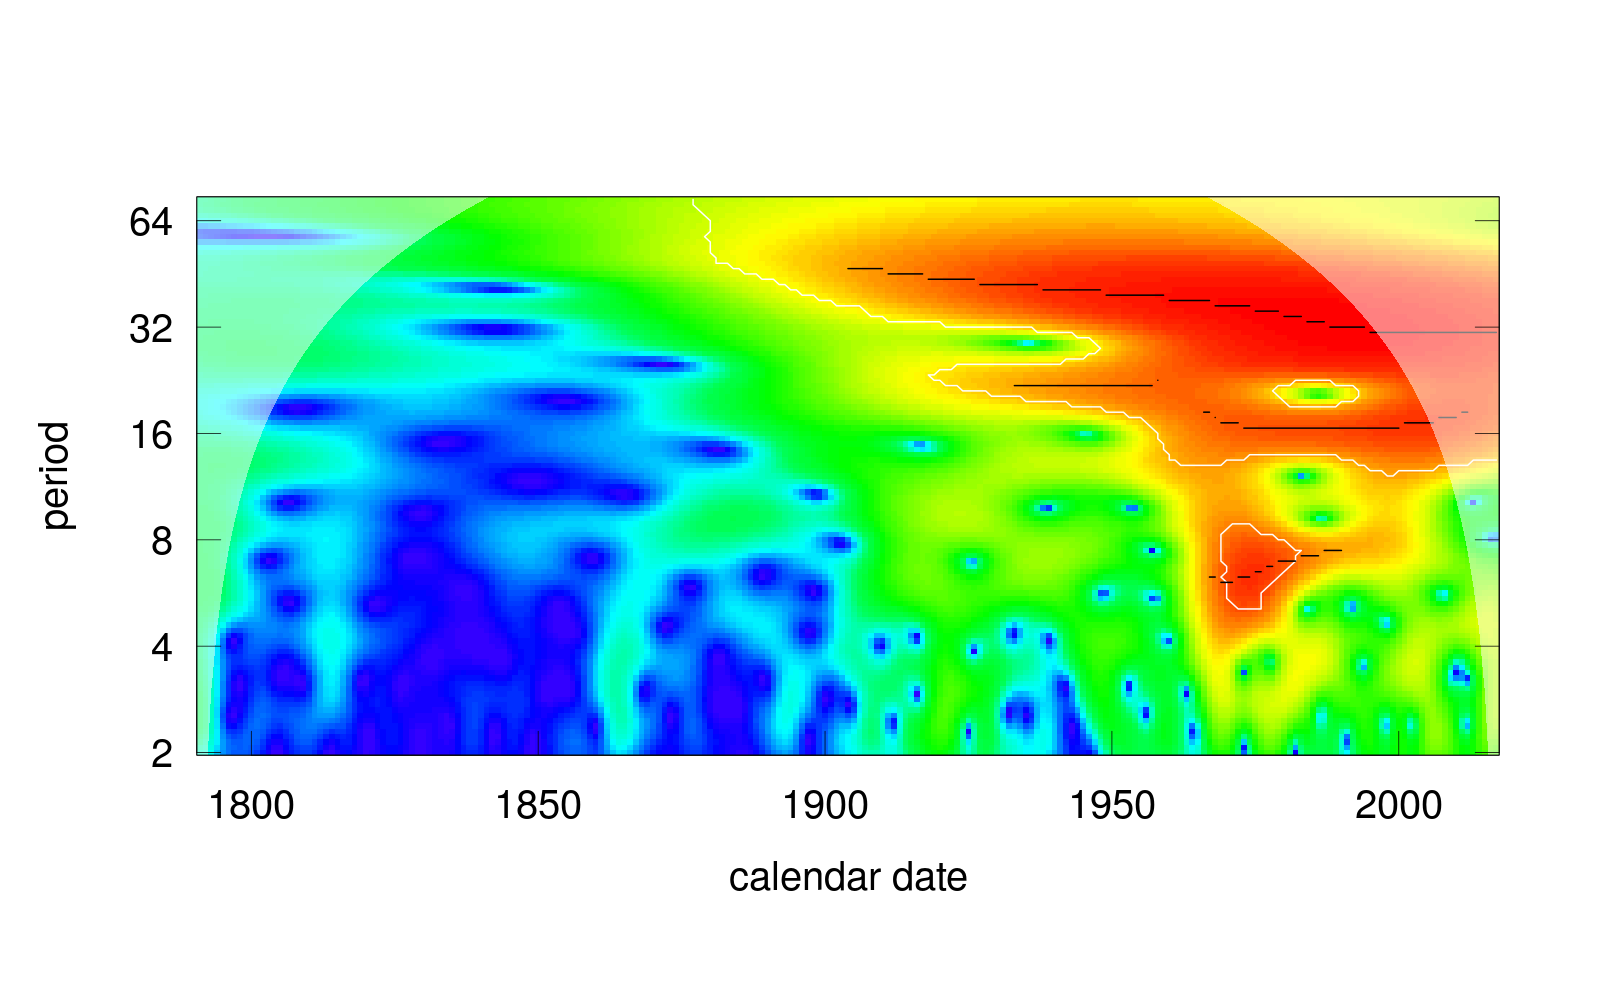
\includegraphics[width=0.75\linewidth]{espectograma_gdp_en.png}
			\label{fig:espect_PBI_a}}
		\subfigure[US log(GDP) spectrogram]{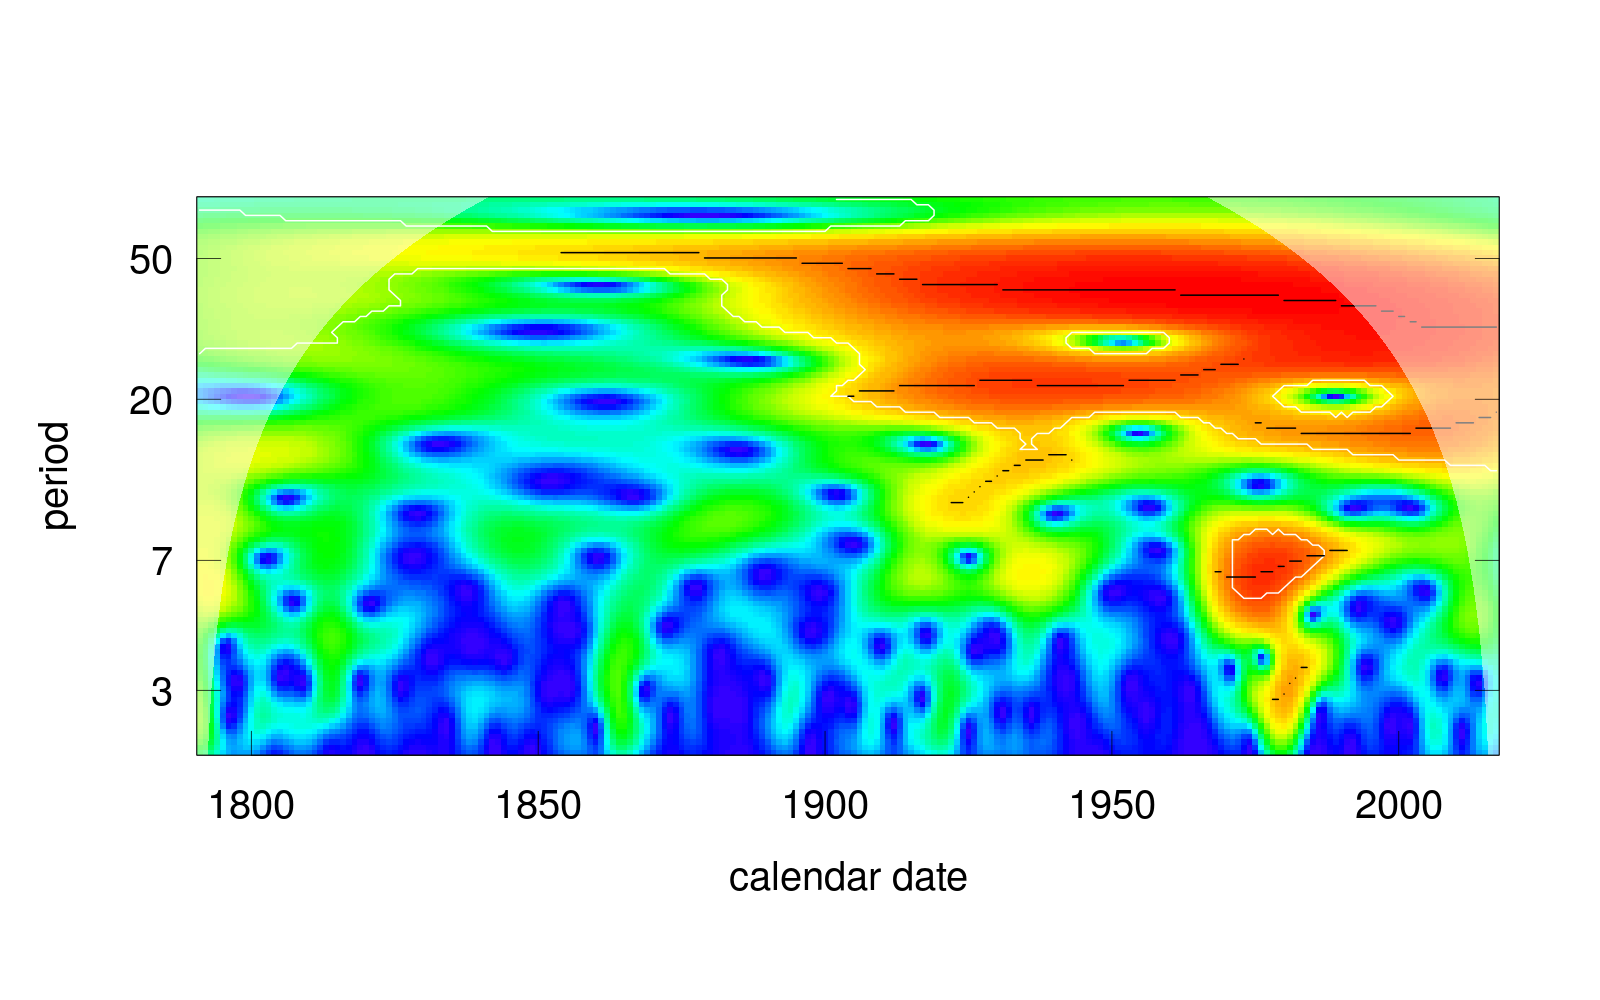
\includegraphics[width=0.75\linewidth]{espectograma_log_gdp_en.png}
			\label{fig:espect_PBI_b}}
		\caption{US GDP in gold. 1790-2017} \label{fig:espect_PBI}
	\end{figure}
	
%	the figure \ref{fig:espect_wg} show the spectrograms of the wage series expressed in gold in \ref{fig:espect_wg_a} and the same taken in log base in \ref{fig:espect_wg_b}. For this series, we can again observe a well-defined long cycle around 50 years, especially if we look at the series taken on a logarithmic basis. This long cycle seems to oscillate between the frequencies of $1/32$ and $1/64$, falling in time. On the other hand, it delimits the second cycle of around sixteen years of extension, and finally a short cycle of between six and eight years. When taking the logistic scale, also appears a cycle of a higher frequency of about three years extension. Consequently, both series seem to yield results in agreement, whether or not they are in the logarithmic base.
	
	
%	\begin{figure}[H]
%		\centering
%		\subfigure[Wage spectrogram]{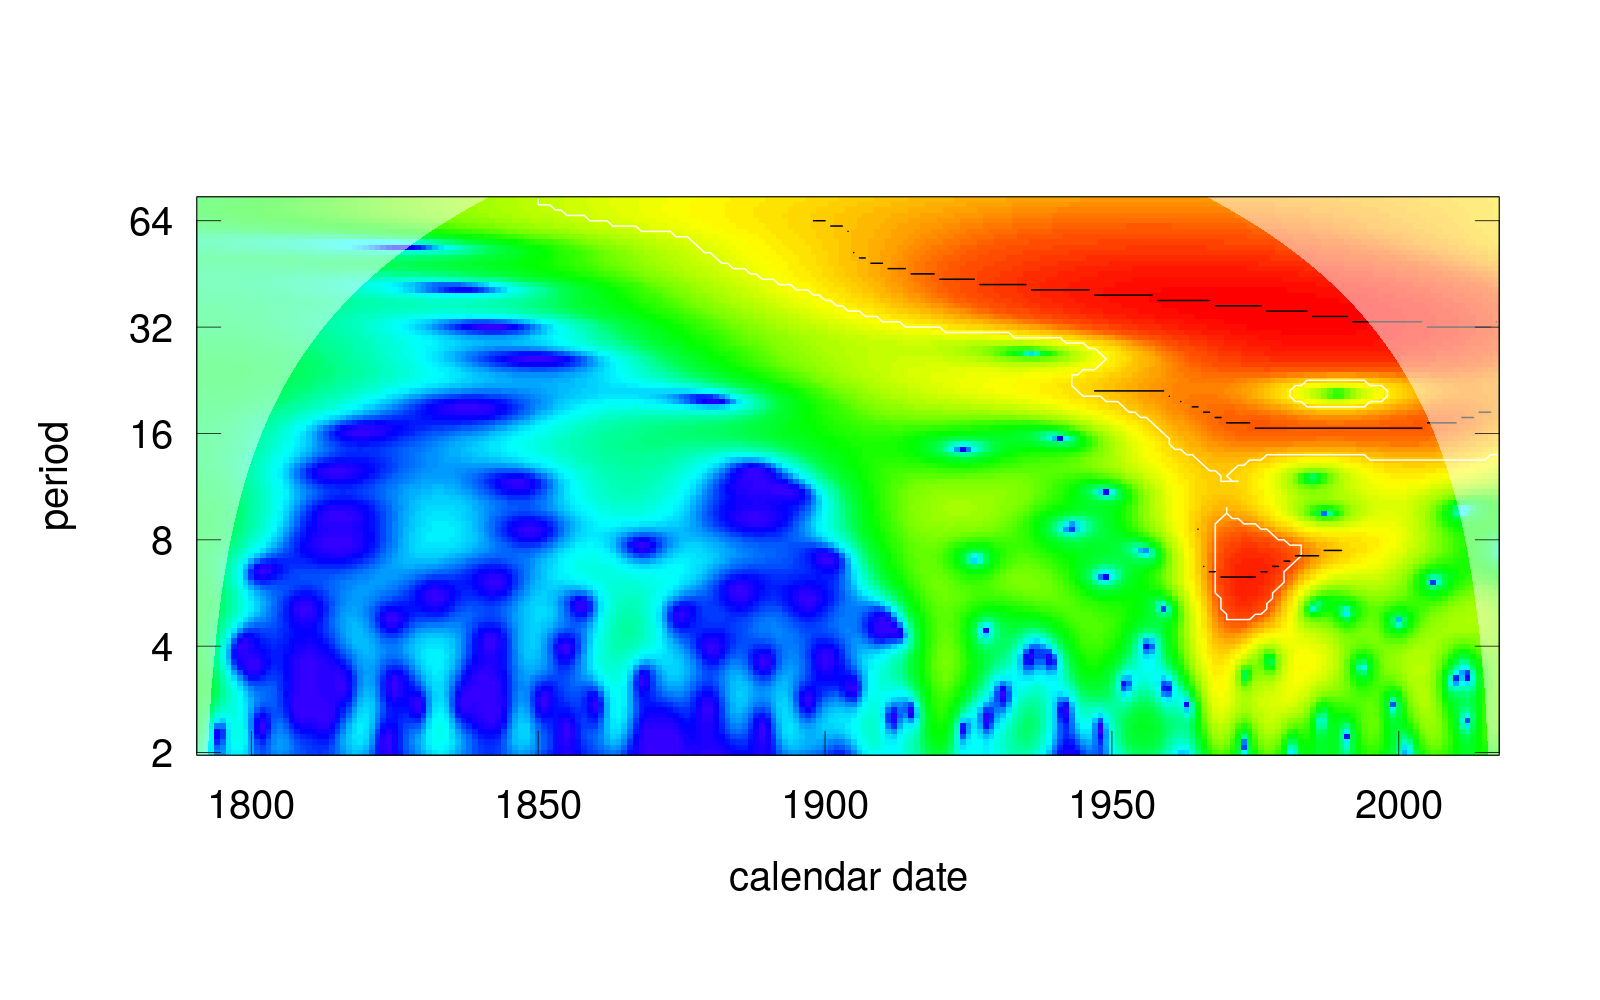
\includegraphics[width=0.75\linewidth]{espectograma_wg_en.png}
%			\label{fig:espect_wg_a}}
%		\subfigure[log(wage) spectrogram]{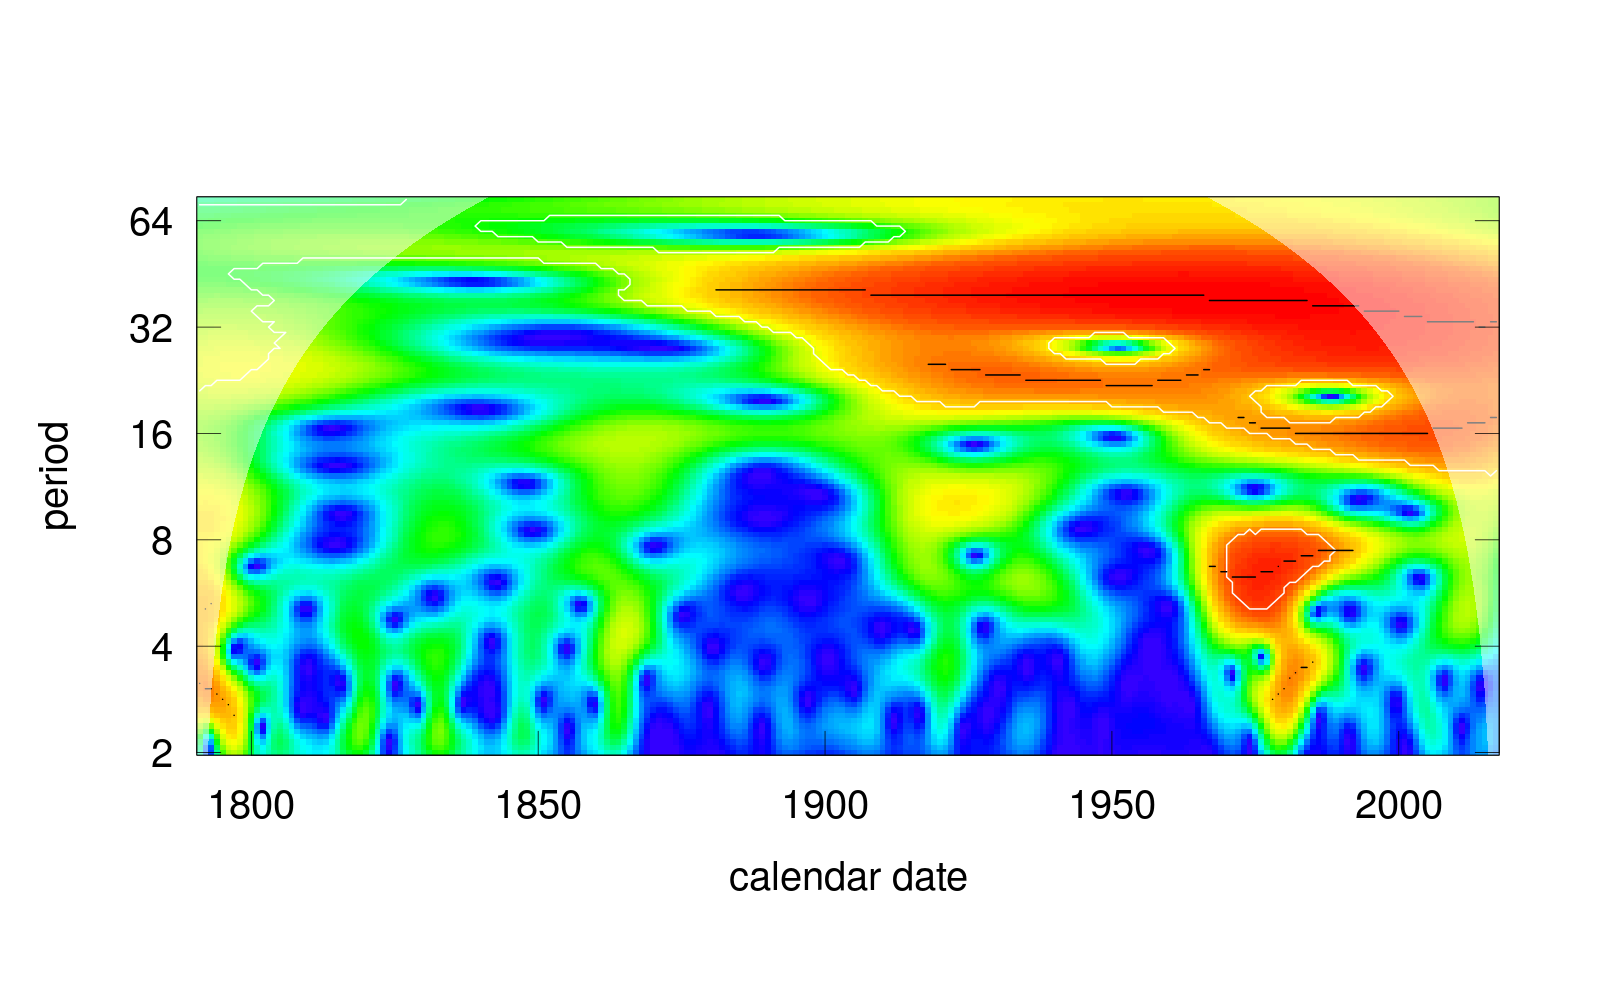
\includegraphics[width=0.75\linewidth]{espectograma_log_wg_en.png}
%			\label{fig:espect_wg_b}}
%		\caption{US wage in gold. 1790-2017} \label{fig:espect_wg}
%	\end{figure}
	
	The figure \ref{fig:espect_uk} shows the GDP series expressed in gold for the United Kingdom between 1700 and 1900. As in the previous series, it is expressed without additional transformations in \ref{fig:espect_uk_a} and in log base in \ref{fig:espect_uk_b}. Unlike the US series, here we can see more clearly the short cycle, around ten years.
	
	\begin{figure}[H]
		\centering
		\subfigure[UK GDP spectrogram]{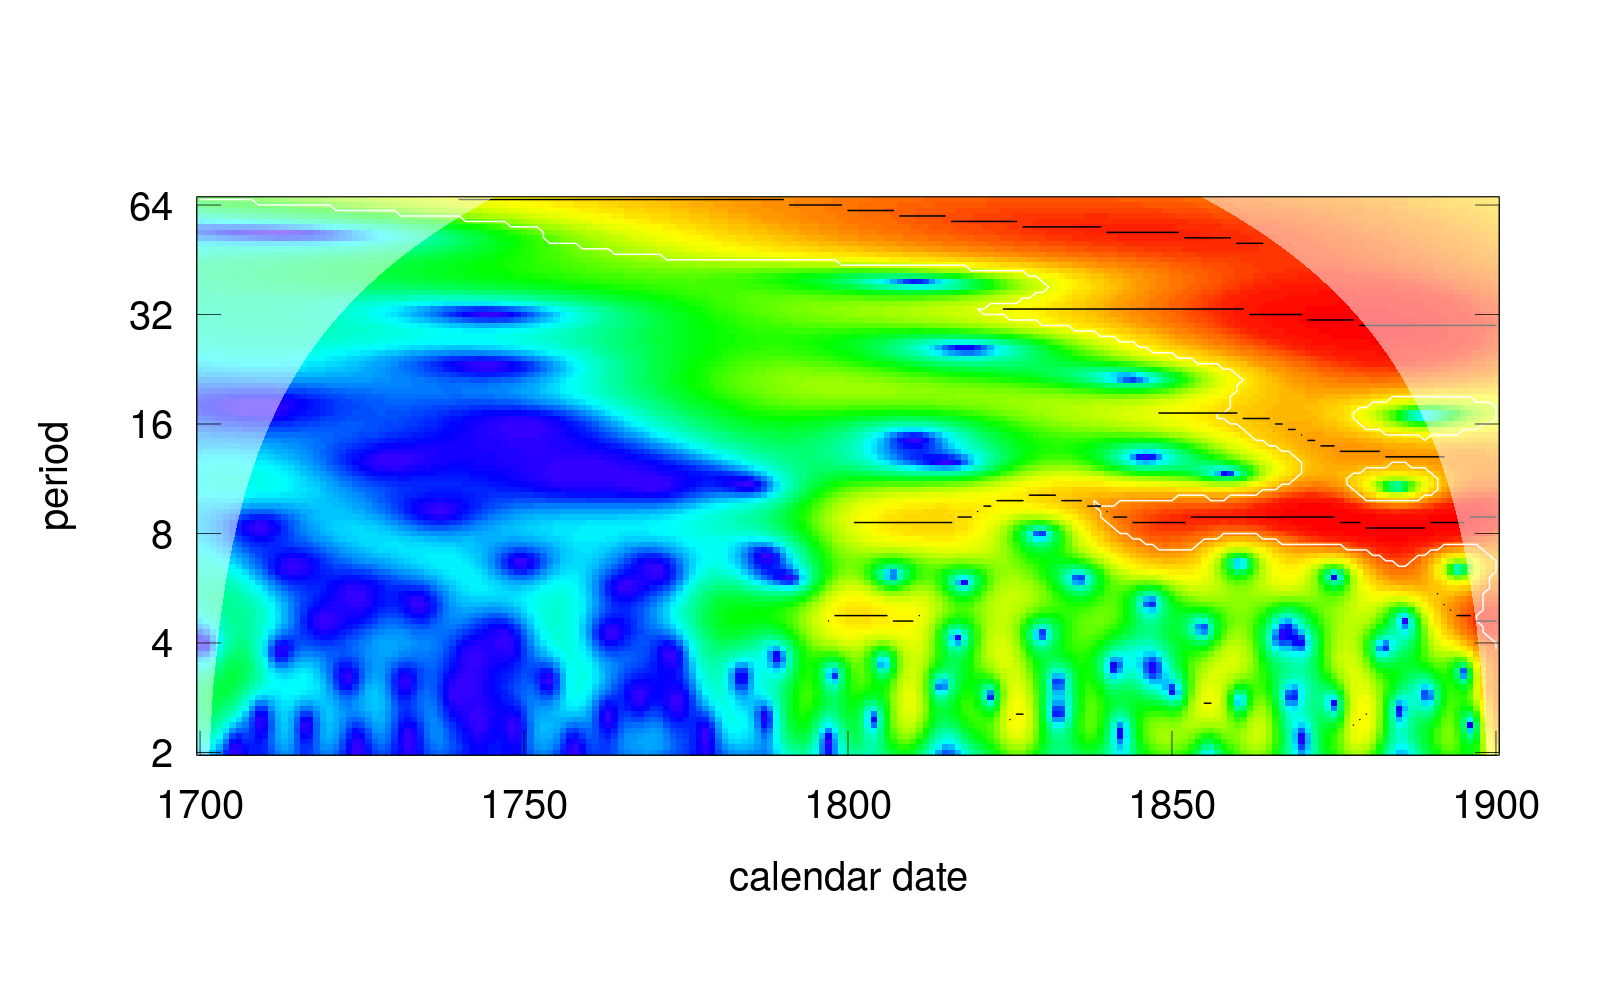
\includegraphics[width=0.75\linewidth]{espectograma_gdp_uk_en.png}
			\label{fig:espect_uk_a}}
		\subfigure[UK log(GDP) spectrogram]{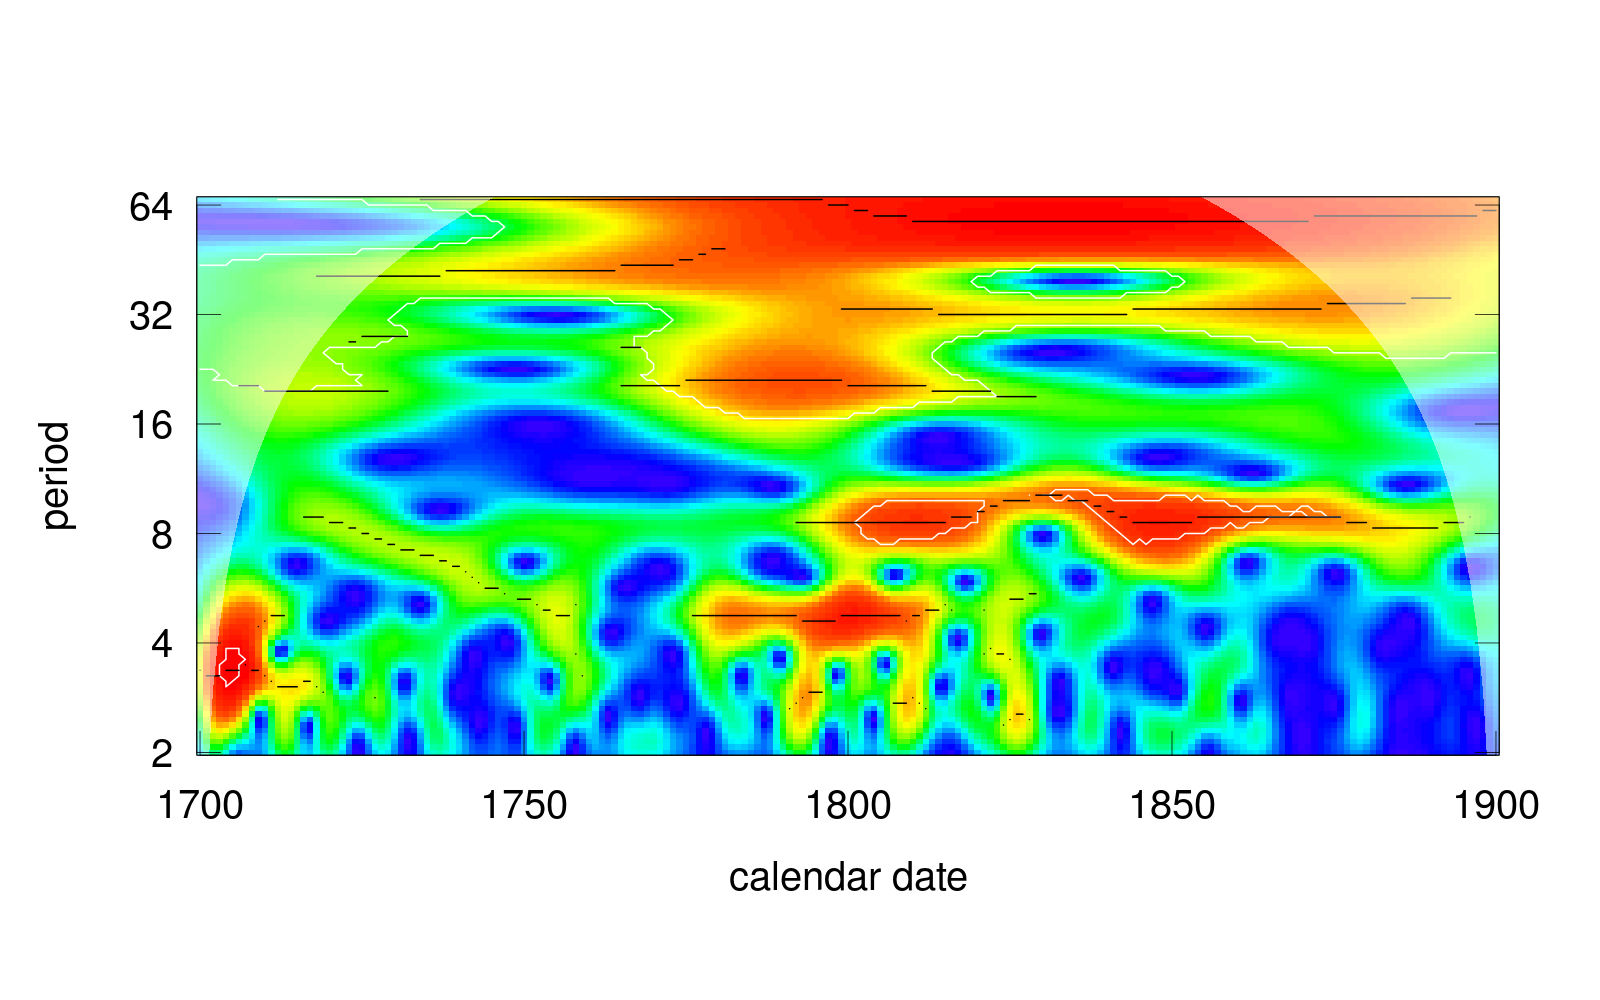
\includegraphics[width=0.75\linewidth]{espectograma_log_gdp_uk_en.png}
			\label{fig:espect_uk_b}}
		\caption{UK GDP in gold. 1700-1900} \label{fig:espect_uk}
	\end{figure}
	
	Besides, another difference that stands out is that in the plots for the UK the effect of the logarithmic transformation is more significant than in the previous series. Thus, in \ref {fig:espect_uk_b} we can observe a multiplicity of cycles that stand out as influential. In particular, the shortest one seems to be around the four years of duration, especially present at the beginning of the series and near 1800. Also highlights the cycle around the eight years of duration, associated in the description made in exploratory data analysis with what we marked as a 10-year cycle. We can note another cycle, of a greater extension around the 20 years, at the beginning of the series and in the environment of 1800, together with a cycle of 30-35 years in the remaining periods. Finally, there is a long cycle around 64 years extension.
	
	It is essential to record the effect produced by the trend of the series on the spectrograms. In section \ref{EDA} the figure \ref{fig:uk_gdp} showed a strong trend effect of the product expressed in gold for the United Kingdom during the eighteenth and nineteenth centuries. This trend did not seem to be linear, and therefore it is of our interest to analyze the possible distortions that this can generate on the spectrograms. In the figure \ref{fig:tendencias} we can see the GDP of the United Kingdom in gold, together with a linear smoothing using a local regressions model \citep{Shyu1992}, and the series resulting from eliminating this trend.
	
	The figure \ref{fig:espectograma_gdp_uk_Tend} shows the spectrogram of the trend calculated on the series. There stands out the period around fifty years, which seems to indicate that what we described before is a simple trend effect hidden in the spectrograms. However, in the figure \ref{fig:espectograma_sin_tend} shows the spectrogram of the series of UK GDP, also expressed in gold but after subtracting the trend. This spectrogram is almost identical to that seen previously in the figure \ref{fig:espect_uk_a}. All this means that the wavelet technique is not affected by the underlying trend of the series analyzed.
	
	\begin{figure}[H]
		\centering
		\subfigure[UK GDP. Millions of ounces of gold, 1700-1900. Trend]{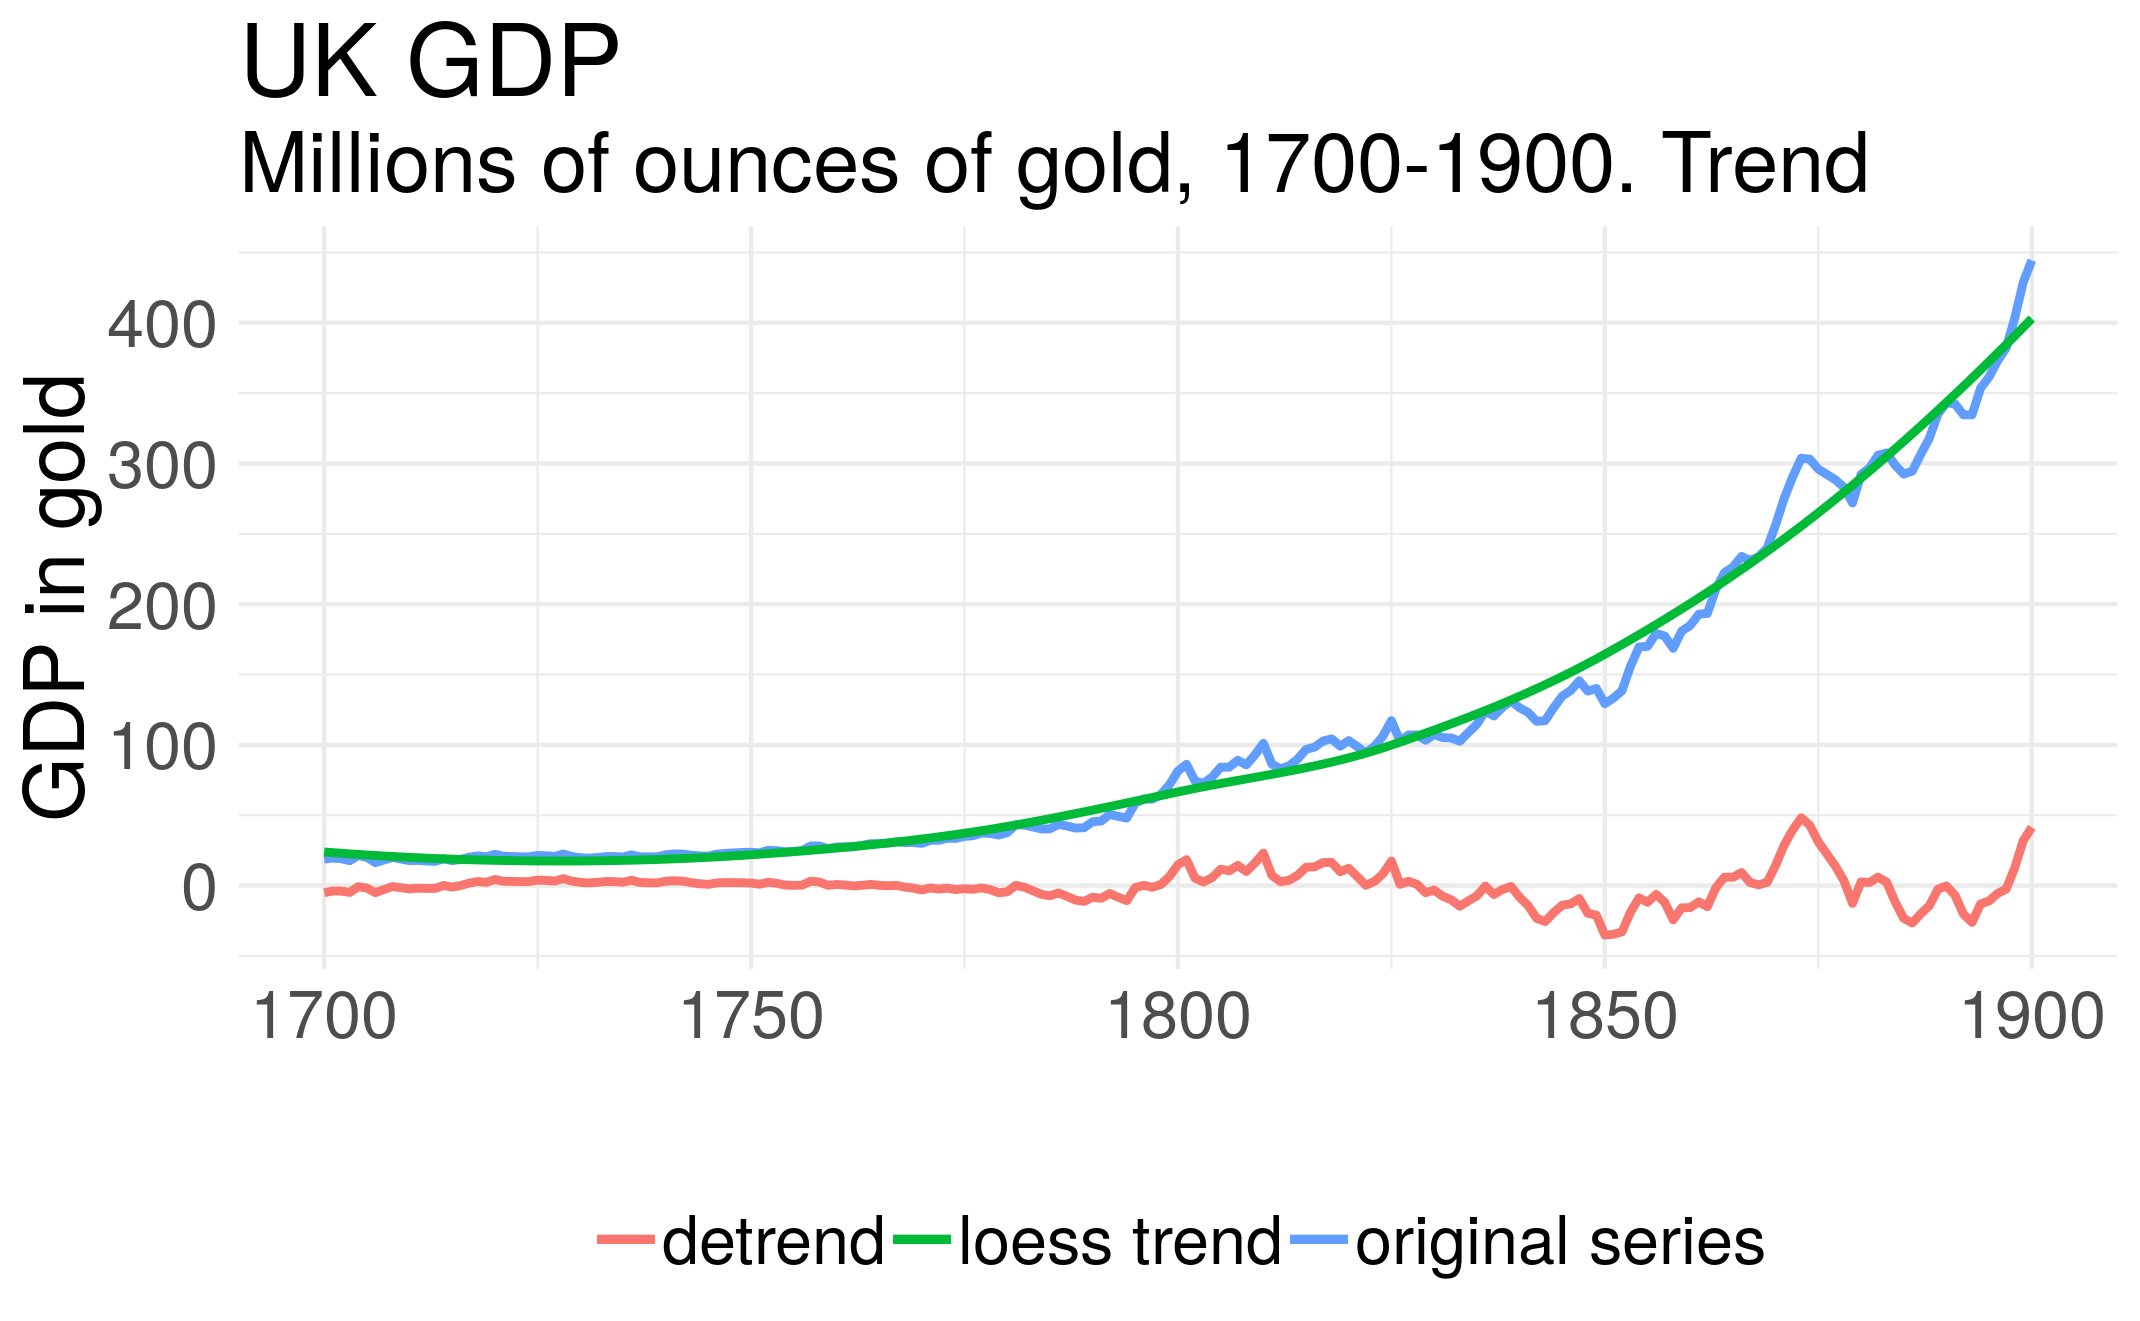
\includegraphics[width=0.75\linewidth]{pbi_uk_tendencias_en.png}
			\label{fig:tendencias}}
		\subfigure[UK GDP spectrogram, trend]{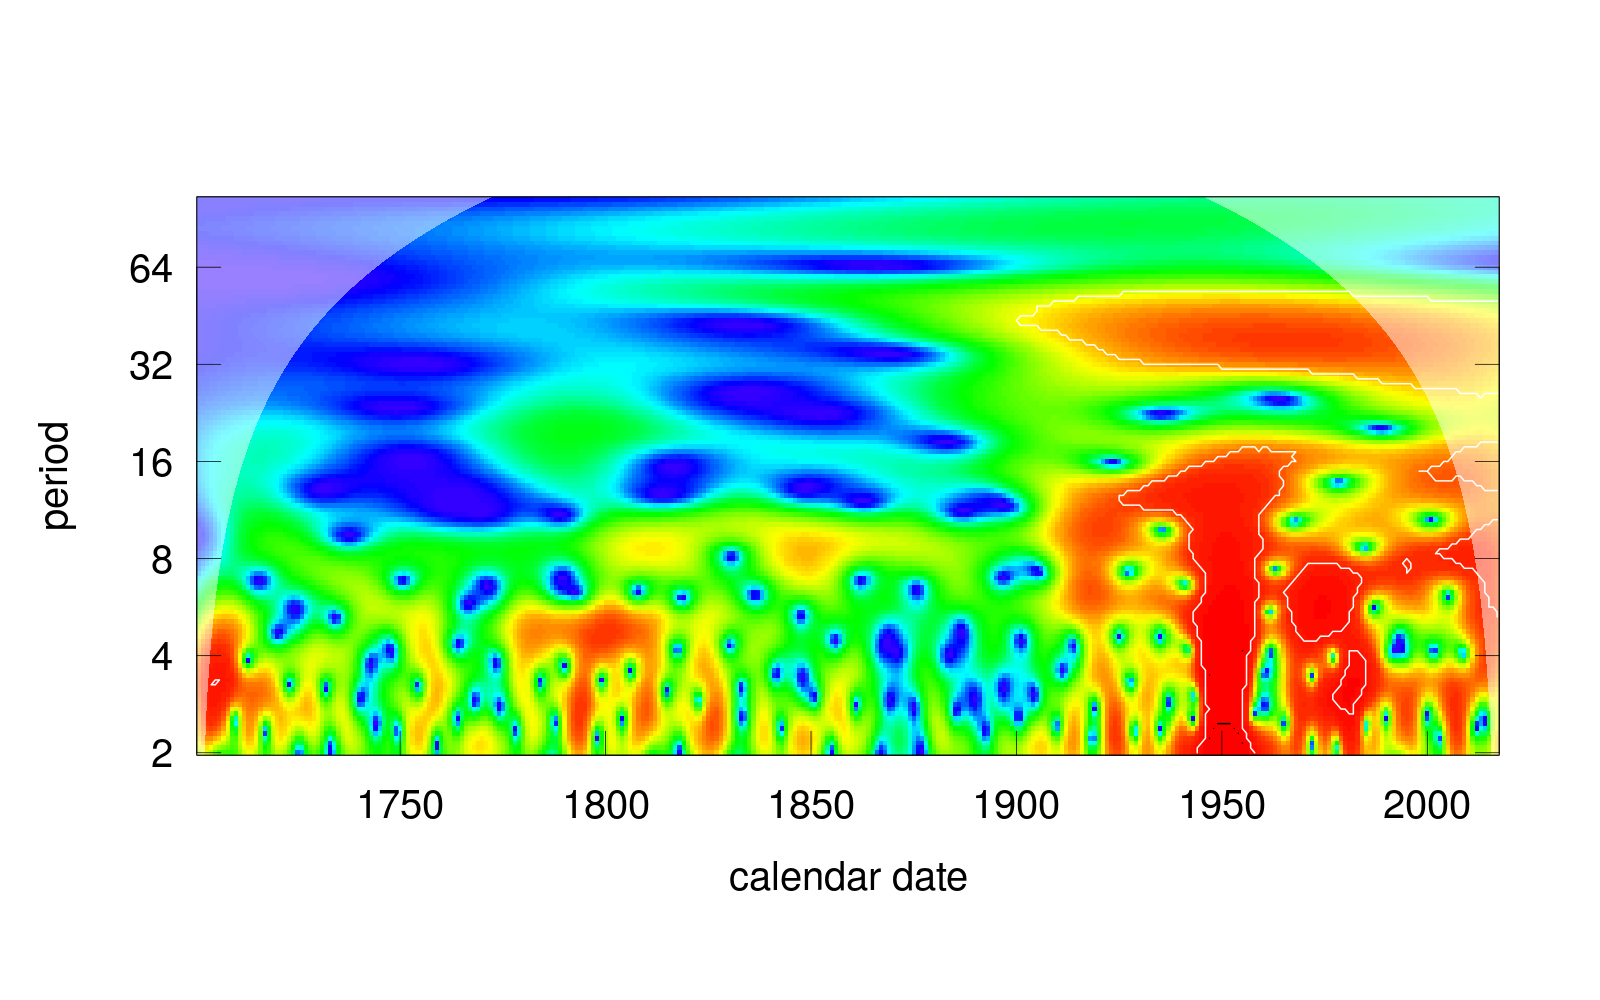
\includegraphics[width=0.48\linewidth]{espectograma_gdp_uk_Tend_en.png}
			\label{fig:espectograma_gdp_uk_Tend}}
		\subfigure[UK GDP spectrogram, detrended]{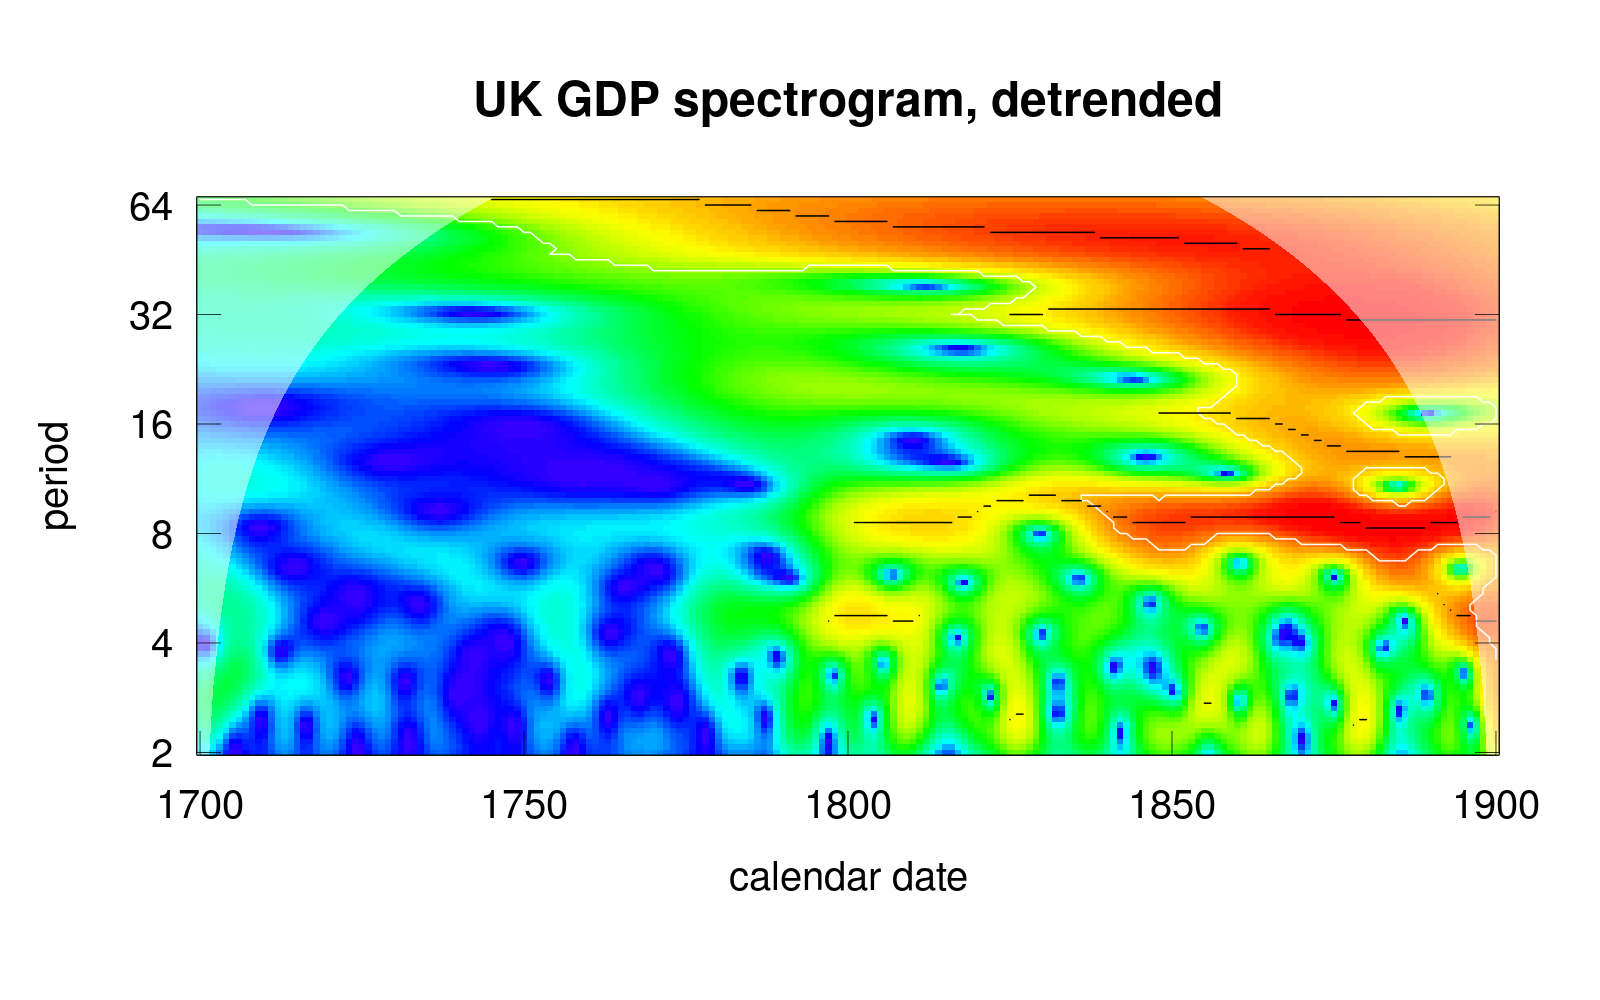
\includegraphics[width=0.48\linewidth]{espectograma_gdp_uk_sinTend_en.png}
			\label{fig:espectograma_sin_tend}}
		\caption{Trend effect} \label{fig:espect_tendencias}
		
	\end{figure}
	
	\section{\uppercase{\textbf{\normalsize{Conclusions}}}}
	
	In this work, we made a tour through the main theoretical approaches concerning the economic cycle and highlighted the importance of empirical analysis. For this latter, we use the GDP and wages of the US between 1790 and 2017, expressed in gold. We also looked at the GDP series for the UK, between 1700 and 1900.
	
	In the exploratory data analysis, we found a substantial correspondence between the breaks of these series and the crises known by the economic historiography. Also, we marked an apparent oscillatory movement that seemed to correspond with the long waves of Kondratieff. For its part, the nineteenth century in the United Kingdom seemed to highlight the crises around the ten years of duration.
	
	Then we explore wavelets-analysis, a tool with which its possible to visualize the correspondence of economic series with cycles of different extensions. The results of this technique showed the existence of three distinct cycles at different frequencies, which correspond to the hypotheses studied on the existence of a short cycle, a medium cycle and a long cycle. It is also important to mention that this tool loses resolution in cycles of very long periods. In this sense, the tool seen does not allow to define precisely the temporal extension of each one of the cycles, but it does provide evidence of their existence.
	
	It is important to note that the objective of this paper is to look for empirical evidence regarding the frequency and amplitude of the cyclical behavior of the economy. We choose the wages and GDP series because they are good approximations of the general economic movement, but they are not the only ones. In turn, statistics have a national base, the GDP is always from a particular country, as well as wages statistics, and so we needed to choose a particular country as an expression of the world economy. In this sense, since the United States is the largest national unit of the world's economy during the 20th century, we begin our analysis with its series. However, while the US economy is a good reflection of the movements of the world economy for the twentieth century, the same does not stand for the nineteenth century. In this sense, it is natural that the general determinations of the economy, such as the cycle, are not fully expressed for that century, and we observe evidence only from 1900 onwards. That is why we complemented the analysis with the GDP of UK for the two preceding centuries.
	
	To conclude, the use of this technique for the study of historical series, widely analyzed by specialized bibliography, seems to be useful to obtain new information from the data used. The results point to the confirmation of the existence of a series of medium and long duration, although the empirical regularity is not sufficient to determine with accuracy the frequency of these cycles. In other words, although the intuition of \cite{kuznets1930secular} and \cite{kondratieff1979long} is confirmed, the results are less promising regarding the possibility of precisely defining the phenomena. Even more, the evidence seems to indicate that the frequency of medium and long duration cycles could vary partially throughout history.
	
	The present work proposes multiple lines of research, especially regarding the use of Wavelets technique in new series, both for series of financial variables, as well as GDP and wages series for other countries.
	
	\mbox{}\\
	
	\bibliography{bibliography.bib}
	
	
	
\end{document}

